\documentclass[a4paper]{report}
\usepackage[bottom=2cm]{geometry}
%\setlength{\belowcaptionskip}{-10pt}
\usepackage[utf8]{inputenc}
\usepackage{fancyhdr}
\pagestyle{fancy}
\usepackage{color}
\usepackage{amsmath, amssymb, graphicx}
\usepackage{bbm}
\usepackage{hyperref}
\usepackage{enumerate}

\usepackage{tabularx, booktabs}
\newcommand\setrow[1]{\gdef\rowmac{#1}#1\ignorespaces}
\newcommand\clearrow{\global\let\rowmac\relax}
\clearrow
\usepackage{multirow}
\usepackage{caption}

\usepackage{helvet} % Helvetica, scaled 95%
\renewcommand\familydefault{\sfdefault}

\usepackage{minted} % Code highlighting
% Python package 'Pygments' required
\usemintedstyle{tango}

\usepackage[style=numeric,giveninits=true]{biblatex}
\addbibresource{refs.bib}

\title{Mathematics Diagnostic Test Project}
\author{Chito Wong}

\begin{document}
\maketitle

\pagenumbering{roman}
\setcounter{page}{1}
\tableofcontents
\newpage

\chapter*{Executive Summary}
\pagenumbering{arabic}
\setcounter{page}{1}
\addcontentsline{toc}{chapter}{Executive Summary}

\chapter{Introduction}

The mathematics diagnostic test (MDT) is applied to new students who are enrolled in courses taught by the School of Mathematics. In 2011, the first generation of MDT (MDT1) was created using Maple T.A., which consists of 32 questions. In 2012, the test was reduced to the form of 20 questions and used in 2012 through 2016. This test is referred as MDT2. Last year, MDT was moved to the STACK online assessment system and replaced Maple T.A. with Moodle \cite{web:mdt}. With this new system, the validity of a student's response is available to access, along with the correctness of the response \cite{web:stack}. 

Over the summer in 2017, two students investigated the data collected on MDT2 in 2013 through 2016, provided suggestions of dropping or adding questions to MDT \cite{lastyear}. This informed the development of a new version of the test, MDT3. The aim of the project this year is to evaluate the performance of MDT3. 

\section{Changes of questions in MDT3}

MDT2 and MDT3 both include 20 questions and each question is scored out of 5 marks. For convenience, the questions from MDT2 are labelled as `Q1', `Q2', etc. (`Q' is short for `Question'), while the questions from MDT3 are labelled as `N1', `N2', etc. (`N' is short for `New'). 

There are three major changes in MDT3: 
\begin{itemize}
\item Based on the suggestions from the report last year, Q2, Q8 and Q11 are removed from MDT, which are replaced by three new questions \cite{lastyear}. 

\item Q4 and Q12 exist in MDT3 with different marking schemes. The new marking schemes are not convertible into the old marking schemes from the previous tests, so they are also treated as new questions. 

\item The questions are in different orders. 
\end{itemize}

For the sake of simplicity, the questions in MDT3 are relabelled, where questions which remain unchanged from MDT2 use the same labels as in MDT2 with prefix `Q' and the other questions keep the labels with prefix `N'. Table~\ref{tab:EDA_groups} shows both labels and the changes of the questions. The letters in column `Type' are the classifications of the questions using taxonomy \cite{taxonomy}, where Type-A questions require routine procedures, Type-B questions are examining existing knowledge in new situations and Type-C questions are logical questions. 

\begin{table}[ht]
  \centering
  \begin{tabular}{llcl}
    \hline
  Label & Relabel & Type & Changes (if any) \\ 
    \hline
    N1 & Q1 & A \\ 
      N2 & Q3 & B \\ 
      N3 & N3 & A & Q4 with different marking schemes\\ 
      N4 & Q5 & A \\ 
      N5 & Q6 & A \\ 
      N6 & Q7 & B \\ 
      N7 & N7 & B & New question \\ 
      N8 & Q9 & A \\ 
      N9 & Q10 & B \\ 
     N10 & N10 & B & New question\\ 
     N11 & N11 & C & New question\\ 
     N12 & N12 & A & Q12 with different marking schemes\\ 
     N13 & Q13 & A \\ 
     N14 & Q14 & B \\ 
     N15 & Q15 & A \\ 
     N16 & Q16 & A \\ 
     N17 & Q17 & A \\ 
     N18 & Q18 & A \\ 
     N19 & Q19 & B \\ 
     N20 & Q20 & B \\ 
     \hline
  \end{tabular}
  \caption{\label{tab:EDA_groups}Labels of questions and corresponding types using taxonomy}
\end{table}

\section{Data exploration and cleaning}

Before analyses are performed on the data retrieved, we should first explore the data, getting basic information of the data and remove any outlier that results in noise contamination. 

\subsection{Raw data}

The raw data of the results of MDT2017 contains the scores and the responses of 926 students in each question. Instead of showing only numerical numbers, the mark of a student scoring in a question may also be a dash (-), indicating the response of the student is not a valid answer. The data also contains the actual response to the questions and the time each student spent in the test. 

The raw data is converted to a numerical version where all dashes are treated as 0 marks for convenience of doing exploratory data analysis. Table~\ref{tab:EDA_dsc_17} shows the summary statistics of the total scores in MDT3, including mean, standard deviation, maximum and minimum. The mean of the total scores is skewed to the left, compared with the median, implying there may exist a large number of students who got low scores in MDT. 

\begin{table}[ht]
  \centering
  \begin{tabular}{rr}
    \hline
 & Value \\ 
  \hline
Min. & 0.00 \\ 
  1st Qu. & 57.75 \\ 
  Median & 72.88 \\ 
  Mean & 69.22 \\ 
  3rd Qu. & 84.50 \\ 
  Max & 100.00 \\ 
  Stand. Dev. & 20.42 \\ 
   \hline
  \end{tabular}
  \caption{\label{tab:EDA_dsc_17}Summary statistics of raw data of MDT3}
\end{table}

The histogram of the total scores (Figure~\ref{fig:EDA_hist_17}) shows that the students scoring 0 to 40 are approximately uniformly distributed. These statistics suggest that unreliable data may be contained in the data set, which needs to be removed. 

\begin{figure}[H]
  \centering
  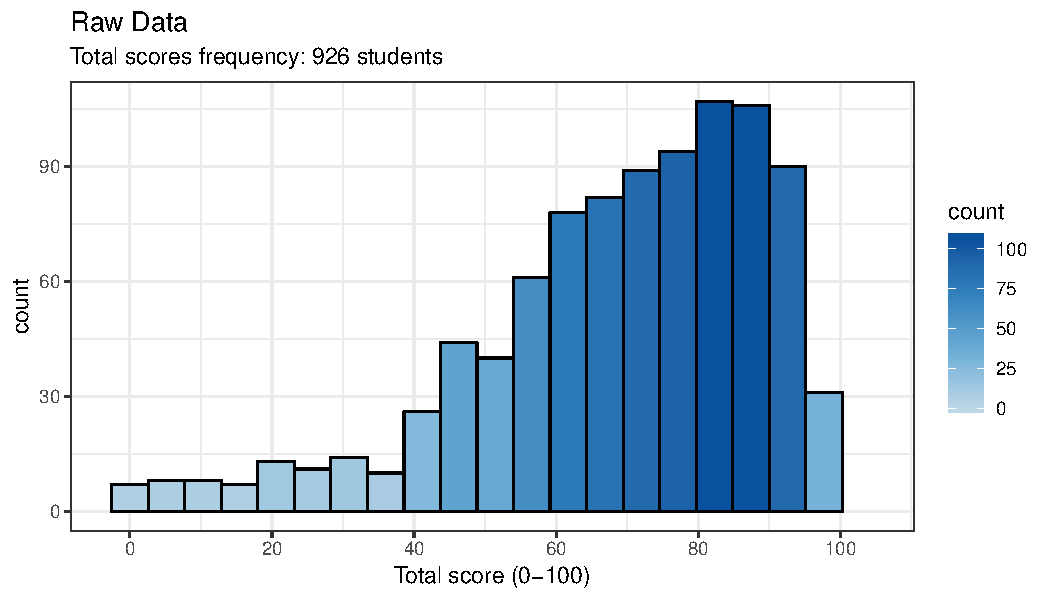
\includegraphics[width=\linewidth]{fig/EDA_hist_17.pdf}
  \caption{\label{fig:EDA_hist_17}Histogram of total test scores of raw data}
\end{figure}

The raw data includes some students more than once, due to some students being allowed a second attempt following technical problems with their first attempt. In such cases, we disregard their worst result. 

% Investigating the raw data set again, I observe that some students occur more than once in the data set, with a relatively low total score and a high total score. These students might take the test twice and their attempts with worse results should be removed. 

\subsection{Cleaning data with previous technique}

The method of data cleaning in the analysis of the last year \cite{lastyear} is 

\begin{enumerate}
\item For students who took the test more than once, consider the attempt with the highest scores only and remove the others; 
\item Eliminate the students who scored three or more zeros in the 5 easiest questions in the second-half of the test; and
\item Add the students scoring more than 30 marks in total back to the sample. 
\end{enumerate}

The aim here is to remove non-serious attempts at the test. 

For consistency, we apply the same cleaning technique on the data from MDT3. Table~\ref{tab:EDA_difficulty} shows the facility of each question by calculating their mean using the data without duplicated students. The five questions with the least facility (or highest mean score) are N11, N12, Q16, Q17 and Q18. 

\begin{table}[ht]
  \centering
  \begin{tabular}{ccccccccccc}
    \hline
    & Q1 & Q3 & N3 & Q5 & Q6 & Q7 & N7 & Q9 & Q10 & N10 \\ 
     \hline
   Difficulty & 4.44 & 3.60 & 4.06 & 3.94 & 1.74 & 3.79 & 1.89 & 4.22 & 3.64 & 2.01 \\ 
      \hline
     \hline
    & N11 & N12 & Q13 & Q14 & Q15 & Q16 & Q17 & Q18 & Q19 & Q20 \\ 
     \hline
   Difficulty & 3.75 & 4.16 & 3.71 & 2.84 & 3.53 & 4.44 & 4.65 & 3.72 & 2.88 & 2.21 \\ 
      \hline
  \end{tabular}
  \caption{\label{tab:EDA_difficulty}Facility of each question}
\end{table}

The number of students removed by using the technique above and the number of students remaining are shown in Table~\ref{tab:EDA_count_clean_legacy}. 

\begin{table}[ht]
  \centering
  \begin{tabular}{rr}
    \hline
   & No. \\ 
    \hline
  All students & 926 \\ 
    Students without duplicated scores & 917 \\
    Total records removed & 42 \\
    Total students removed &  33 \\ 
    Students remaining for further analysis & 884 \\ 
     \hline
  \end{tabular}
  \caption{\label{tab:EDA_count_clean_legacy}Cleaning the data using the same method as in 2017 report}
\end{table}

The summary statistics and the histogram are shown in Table~\ref{tab:EDA_dsc_17clean_legacy} and Figure~\ref{fig:EDA_hist_17clean_legacy}. The difference between the mean and the median of the total scores is reduced and the lump of the students scoring lower than 40 marks in the histogram seems to have been removed properly. 

\begin{table}[ht]
  \centering
  \begin{tabular}{rr}
    \hline
   & Value \\ 
    \hline
  Min. & 12.50 \\ 
    1st Qu. & 60.00 \\ 
    Median & 73.94 \\ 
    Mean & 71.32 \\ 
    3rd Qu. & 85.00 \\ 
    Max & 100.00 \\ 
    Stand. Dev. & 17.53 \\ 
     \hline
  \end{tabular}
  \caption{\label{tab:EDA_dsc_17clean_legacy}Summary statistics of data after cleaning using previous technique}
\end{table}

\begin{figure}[H]
  \centering
  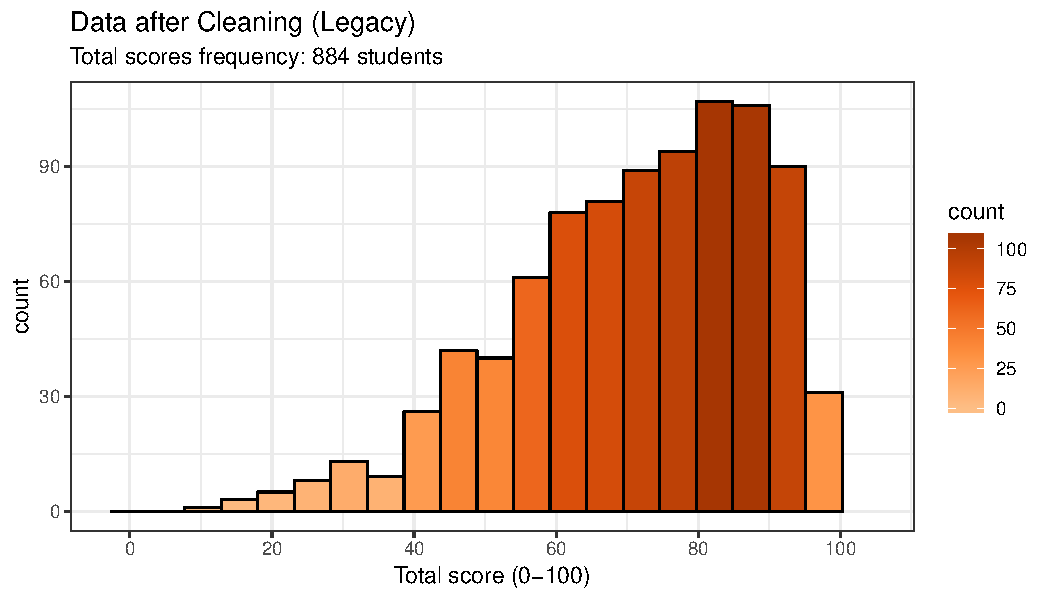
\includegraphics[width=\linewidth]{fig/EDA_hist_17clean_legacy.pdf}
  \caption{\label{fig:EDA_hist_17clean_legacy}Histogram of total test scores of data after cleaning using previous technique}
\end{figure}

\subsection{Cleaning data with new technique}

Although the technique of removing unreliable data from last year works well on the data from MDT3, there is a problem of the technique: it considers only the marks of the questions but ignores the validity of the responses, which is available for the data from MDT3. 

The frequencies of the numbers of valid responses of the test given by the students removed are shown in Table~\ref{tab:EDA_validresp_legacy}. There are over a third of the students removed giving more than 10 valid responses in the test, whether or not these were correct. %Among their responses to the questions they scored 0 marks but valid in the test, all the answers given are meaningful though they are incorrect. 

\begin{table}[ht]
  \centering
  \begin{tabular}{rcccccccccccc}
    \hline
  Number of valid responses & 2 & 4 & 5 & 6 & 7 & 9 & 10 & 11 & 13 & 14 & 15 & 18 \\
  \hline 
    Frequency & 2 & 4 & 5 & 5 & 2 & 1 & 2 & 3 & 2 & 5 & 1 & 1 \\ 
     \hline
  \end{tabular}
  \caption{\label{tab:EDA_validresp_legacy}Frequencies of the numbers of valid responses given by the students removed}
\end{table}

We therefore modify the data cleaning method to make use of the validity data: 
% With the data of validity of responses I have, the method used to eliminate students can therefore be modified as

\begin{enumerate}[\indent2*.]
\item Eliminate the students who gave three or more invalid responses in the 5 easiest questions in the second-half of the test. 
\end{enumerate}

The number of students removed by using the new technique are shown in Table~\ref{tab:EDA_count_clean}. 

\begin{table}[ht]
  \centering
  \begin{tabular}{rr}
    \hline
   & No. \\ 
    \hline
  All students & 926 \\ 
    Students without duplicated scores & 917 \\ 
    Total records removed &  30 \\ 
    Total students removed &  21 \\ 
    Students remaining for further analysis & 896 \\ 
     \hline
  \end{tabular}
  \caption{\label{tab:EDA_count_clean}Cleaning the data using the new method}
\end{table}

The summary statistics in Table~\ref{tab:EDA_dsc_17clean} and the histogram in Figure~\ref{fig:EDA_hist_17clean} both show satisfying results that the unreliable data are eliminated properly and the distribution seems to be Normal. 

\begin{table}[ht]
  \centering
  \begin{tabular}{rr}
    \hline
    & Value \\ 
     \hline
   Min. & 5.00 \\ 
     1st Qu. & 59.50 \\ 
     Median & 73.75 \\ 
     Mean & 70.61 \\ 
     3rd Qu. & 85.00 \\ 
     Max & 100.00 \\ 
     Stand. Dev. & 18.46 \\ 
      \hline
  \end{tabular}
  \caption{\label{tab:EDA_dsc_17clean}Summary statistics of clean data of MDT3}
\end{table}

\begin{figure}[H]
  \centering
  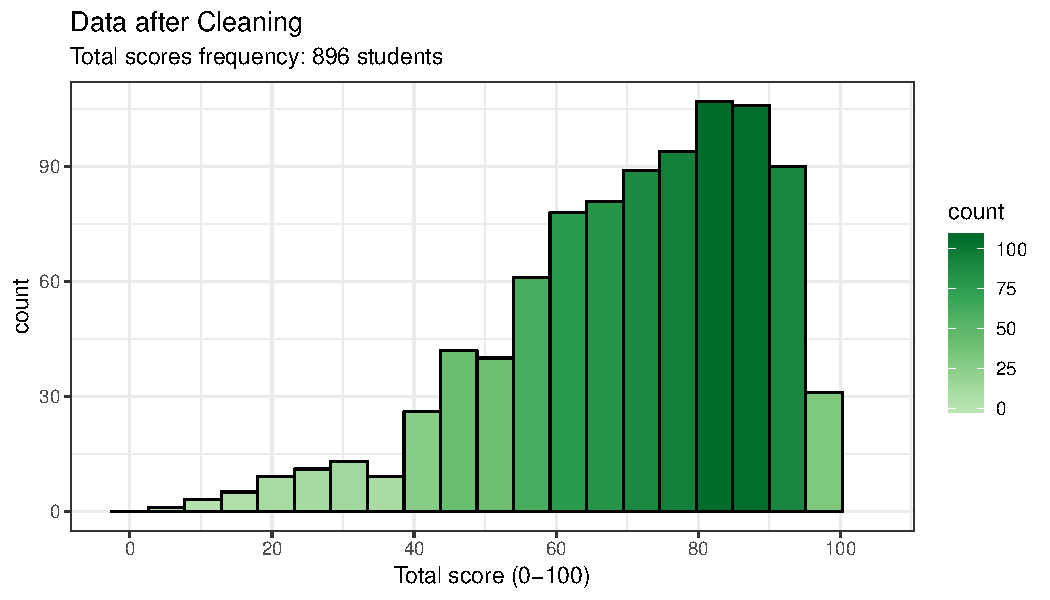
\includegraphics[width=\linewidth]{fig/EDA_hist_17clean.pdf}
  \caption{\label{fig:EDA_hist_17clean}Histogram of total test scores of data after cleaning using new technique}
\end{figure}

The frequencies of the numbers of valid responses of the test given by the students removed by the new technique are shown in Table~\ref{tab:EDA_validresp}. Most of these students did not give more than 10 valid responses, so they can be considered to have failed to complete the test to the best of their ability. 

\begin{table}[ht]
  \centering
  \begin{tabular}{rcccccccc}
    \hline
  Number of valid responses & 2 & 4 & 5 & 6 & 7 & 9 & 10 & 11 \\ 
    \hline
    Frequency & 2 & 4 & 5 & 5 & 2 & 1 & 1 & 1 \\ 
     \hline
  \end{tabular}
  \caption{\label{tab:EDA_validresp}Frequencies of the numbers of valid responses given by the students who are removed by the new cleaning technique}
\end{table}

\subsection{Comparison of the cleaning methods}

From the results of the previous sections, 33 students are removed using the same technique as last year from a data set with 917 students, while 21 are removed using the new technique which considers the validity of responses. This can be seen in the confusion matrix in Table~\ref{tab:EDA_cm}. A detailed introduction to the confusion matrix and evaluation of binary classifier can be seen in Section~\ref{subsec:cm}. 

\begin{table}[ht]
  \centering
  \begin{tabular}{r|cc|c}
    \hline
 & Removed by old method & Kept by old method & Sum \\ 
  \hline
Removed by new method & 21 & 0 & 21 \\ 
  Kept by new method & 12 & 884 & 896 \\ 
  \hline
  Sum & 33 & 884 & 917 \\ 
   \hline
  \end{tabular}
  \caption{\label{tab:EDA_cm}Confusion matrix based on two cleaning methods}
\end{table}

If we consider the new cleaning method to be ideally a perfect classification of reliable and unreliable data and as a reference classification, the accuracy of the old cleaning method can be calculated as 

$$ACC = \frac{TP + TN}{TP + FN + TN + FP} \text{, }$$

\noindent
where TP (True Positive) are those who are removed by the new method and the old method removes them, FN (False Negative) are those who are removed by the new method but are not be removed by the old method, and TN (True Negative) and FP (False Positive) are analogous to TP and FN. The accuracy of the old method is 98.7\% which is quite high, suggesting that two cleaning methods are similar. 

We therefore use the new method as the method of cleaning data from MDT3 because it makes the most of the raw data and keeps much sensible data. Although this method cannot be applied to the data from the previous tests because of a lack of validity information, this method should be used consistently on the data from the future tests, unless a better method is discovered. 

\section{Data from MDT2}

In this report, analyses performed are using the data of MDT taken in both 2017 and before 2017. There are two different kinds of data of MDT taken before 2017, including a combined data set of MDT2013, MDT2014, MDT2015 and MDT2016, and four data sets of these four years separately. 

The combined data set was used in the report last year and will be used in this report. This data set will be cleaned by the old method, i.e. the method used in the analyses last year, for consistency. The tests from year 2013 to 2016 were the same and the data does not contain the year when the students took the test, so only the attempt with the highest total score is considered if a student took the test in more than one year. This is consistent with the analyses conducted last year. 

The separated data sets will be used to analyse the growth of ability of the students each year. These data sets will also be cleaned by the old method. However, the students who took the tests in more than on year will be considered to be `different' and their best results in each year will all be kept. The summary statistics are shown in Table~\ref{tab:EDA_dsc_13to16_clean} and the histogram of the total scores are shown in Figure~\ref{fig:EDA_hist_13to16_clean}, where an increase in the mean of the total scores can be seen, indicating the ability of the new students increases each year. 

\begin{table}[ht]
  \centering
  \begin{tabular}{rrrrr}
    \hline
    & MDT2 (2013) & MDT2 (2014) & MDT2 (2015) & MDT2 (2016) \\ 
    \hline
  Min. & 10.00 & 13.75 & 20.50 & 20.50 \\ 
    1st Qu. & 57.50 & 58.25 & 61.75 & 67.75 \\ 
    Median & 70.00 & 71.00 & 76.00 & 79.50 \\ 
    Mean & 68.96 & 69.56 & 72.93 & 77.15 \\ 
    3rd Qu. & 82.50 & 82.50 & 87.00 & 89.00 \\ 
    Max & 100.00 & 100.00 & 100.00 & 100.00 \\ 
    Stand. Dev. & 17.79 & 17.53 & 17.41 & 15.41 \\ 
     \hline
  \end{tabular}
  \caption{\label{tab:EDA_dsc_13to16_clean}Summary statistics of cleaned data from year 2013 to 2016}
\end{table}

\begin{figure}[H]
  \centering
  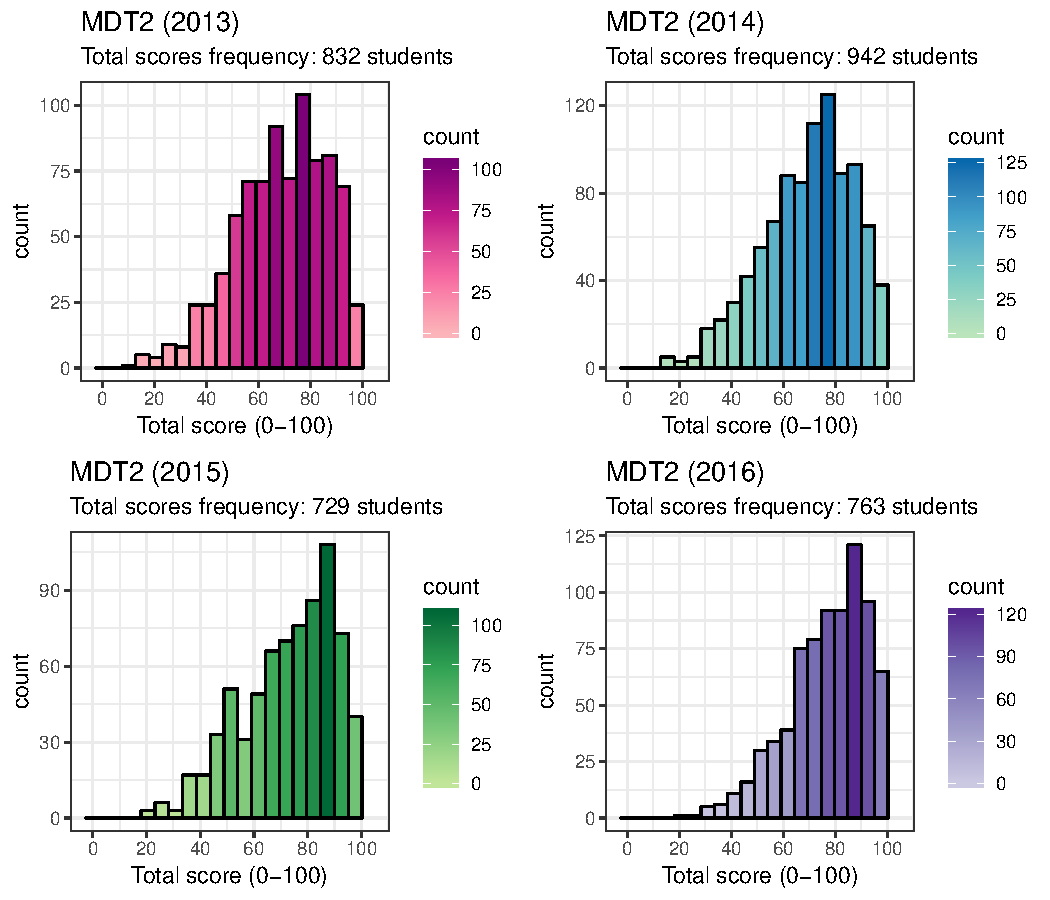
\includegraphics[width=\linewidth]{fig/EDA_hist_13to16_clean.pdf}
  \caption{\label{fig:EDA_hist_13to16_clean}Histogram of total test scores of data after cleaning using new technique}
\end{figure}


\chapter{Partial Credit Model}

An item response theory model is a method of assessing the relation between categorical observable variables and continuous latent variables \cite{lvm}. In our case, we theorise a relation between students' mathematical ability (continuous latent variable) and their performance on the MDT, as measured by their question scores (categorical observed variables). A dichotomous item response theory model which has only two alternative responses (e.g. correct or incorrect), is a simple model and can be well-understood and easily implemented. This model was used in the last year. However, our data is polytomous, since partial marks are available. 

For item response data with multiple categories, polytomous IRT models need to represent the relation. There are several polytomous IRT models \cite{IRT}, but for our data , the partial credit model (PCM) is appropriate. In \texttt{R}, both \texttt{ltm} and \texttt{mirt} packages can be used to fit PCM. 

\section{Assumptions}

As an IRT model, PCM entails the same assumptions as other IRT models. One of the assumptions is the local independence of items, i.e. responding to a question is not related to any other questions. Students are also expected to work independently and not discuss the test with others. The set of latent variables is the only variable that explains the correlation between each pair of observed items. 

The dimensionality of the latent variables should also be identified before applying PCM. This is often investigated with factor analysis \cite{mirt}. 


\section{Models}

The generalised partial credit model (GPCM) with traditional parameterisation \cite{IRT} is defined as

$$P_{ik}(\theta)= \frac{\displaystyle \exp \sum_{c=0}^{k} a_i (\theta-\delta_{ic})}{\displaystyle \sum_{r=0}^{m_i} \left[ \exp \sum_{c=0}^r a_i (\theta-\delta_{ic}) \right]} \text{ for } k=0,1,\ldots,m_i \text{, with } \sum_{c=0}^0 a_i (\theta-\delta_{ic}) = 0 \text{, }$$

\noindent
where $P_{ik}(\theta)$ denotes the probability of responding in category $k$ for item $i$, given the latent ability $\theta$; $a_i$ are the slope parameters; $\delta_{ic}$ are the item-category parameters, representing the relative difficulty between category $c-1$ and $c$; $m_i$ is the number of categories for item $i$, excluding $0$. 

Introducing an integer scoring function $T_{ik}$, which is the score of each category for item $i$ \cite{gpcmiic}, the model can be rewritten as 

$$P_{ik}(\theta) = \frac{\exp (T_{ik} \cdot a_i \theta + d_{ik})}{\displaystyle \sum_{c=0}^{m_i} \exp (T_{ic} \cdot a_i \theta + d_{ic})} \text{. }$$

For the GPCM with traditional parameters, the scoring function $T_{ik} = k$ for each item $i$, i.e. the difference in score between the consecutive categories is fixed at $1$. Therefore, the parameters $d_{ik}$ in the alternative model are equivalent to $\sum_{c=0}^k (-a_i \delta_{ic})$. 

The scoring function $T_{ik}$ can be modified to cooperate with items with non-constant difference between the consecutive categories. For example, if the possible marks for an item are 0, 2, 3 and 5 out of 5, the modified scoring function $\boldsymbol T_i$ can be written as $\boldsymbol T_i = (0,2,3,5)^T$. \texttt{mirt} can fit GPCM with modified scoring function, by adding extra function parameter \texttt{gpcm\_mat} \cite{mirt}. However, it only gives parameter estimates but cannot calculate further inferences described below. 

The partial credit model (PCM) is a constrained GPCM with equal item slope parameters $a_i$ fixed at $1$. This model is called `Rasch' in both \texttt{ltm} and \texttt{mirt} packages. Alternatively, the item slope parameters can be assumed equal but estimated in the model `1PL'. 

For multidimensional cases with two or more latent traits (sometimes also called factors), the model is defined as 

$$P_{ik}(\boldsymbol\theta) = \frac{\displaystyle \exp \left( T_{ik} \cdot \boldsymbol{a}_i^T \boldsymbol\theta + d_{ik} \right)}{\displaystyle \sum_{c=0}^{m_i} \exp \left( T_{ic} \cdot \boldsymbol{a}_i^T \boldsymbol\theta + d_{ic} \right)} \text{, }$$

\noindent
where $\boldsymbol{a}_i$ is a vector of item slope parameters on each latent trait and $\boldsymbol\theta$ is a vector of latent traits values. 

\section{Inferences}

\subsection{Expected score function}

The expected score for each item given uni-dimensional ability $\theta$, is the weighted sum of all the probabilities of responses, where the weights are given by the scoring functions $T_{ik}$ for $k=0,1,\ldots,m_i$, i.e. 

$$\bar{T}_i (\theta) = \sum_{k=1}^{m_i} T_{ik} P_{ik}(\theta) \text{. }$$

\subsection{Information function}
The item information function for polytomous IRT \cite{gpcmiic}, including GPCM, with is defined as

$$I_i(\theta) = \sum_{k=1}^{m_i} P_{ik}(\theta) [-\frac{\partial^2}{\partial \theta^2} P_{ik}(\theta)] = a_i^2 \sum_{k=1}^{m_i} [T_{ik} - \bar{T}_i(\theta)]^2 P_{ik}(\theta) \text{. }$$

The test information function is the sum of the item information functions, i.e. 

$$I(\theta) = \sum_i I_i(\theta) \text{. }$$

The information functions are used for predicting the accuracy of measuring the latent ability \cite{VisualIRT}. The standard error of measurement (SEM) is defined as the square root of the reciprocal of the test information function, i.e. 

$$SEM(\theta) = \sqrt{\frac{1}{I(\theta)}} \text{. }$$

\subsection{Ability estimates}

The ability estimation (or factor score) method used in the report is expected a-posterior (EAP). The EAP scores are defined as

$$\mathrm{EAP}(\theta | \boldsymbol k) = \int \theta p(\theta|\boldsymbol k) d\theta \text{, }$$

\noindent
where $\boldsymbol k$ is the response pattern, $p(\theta|\boldsymbol k)$ is the posterior probability. The posterior probability is calculated by the Bayes' theorem

$$p(\theta|\boldsymbol k) = \frac{p(\boldsymbol k|\theta) p(\theta)}{p(\boldsymbol k)} \text{, }$$

\noindent
where the prior distribution $p(\theta)$ is a standard normal distribution. 

\subsection{Goodness of model-fit}

The Pearson's $\chi^2$ statistic is defined as 

$$\chi^2 = \sum_{r=1}^{n} \frac{[O(r) - E(r)]^2}{E(r)} \text{, }$$

\noindent
where $r$ represents a response pattern, $n$ represents the number of different response patterns, $O(r)$ and $E(r)$ are the observed and expected frequencies. 

The Pearson's $\chi^2$ statistic is used a goodness-of-fit statistic to test the following hypothesis: 

$$H_0 \text{: There is no significant difference between observed and fitted values, }$$

\noindent
against

$$H_1 \text{: There is a significant difference between observed and fitted values, }$$

\noindent
where the observed and fitted values are the observed and expected frequencies of each response pattern of the data. 

However, the approximation of the $\chi^2$ is not reliable when the expected frequencies are too low. Because we have a large number of items, and several of them have many possible responses, the expected frequencies of many response patterns are less than 1, so a parametric Bootstrap approximation is used to assess the goodness of fit. 

The algorithm of the Bootstrap test \cite{ltm} is implemented as 

\begin{enumerate}[Step 1]
\item Compute the ordinary statistic $\chi^2$; 
\item \label{alg:bootstrap_start}Simulate new parameters $\beta^*$ from the multivariate normal distribution $N(\hat\beta, \Sigma(\hat\beta))$, where $\hat\beta$ is the vector of the maximum likelihood estimates of all parameters $a_i$ and $\delta_{ic}$, $\Sigma(\hat\beta)$ is the variance-covariance matrix of the parameters; 
\item Simulate new response patterns using the simulated $\beta^*$; 
\item \label{alg:bootstrap_end}Fit the PCM to the simulated response patterns and compute the corresponding statistic $\chi^2_{i}$; and
\item Repeat Step~\ref{alg:bootstrap_start} to Step~\ref{alg:bootstrap_end} $B$ times and compute the $p$-value using $\displaystyle \frac{1 + \sum_{i=1}^B \mathbbm{1}(\chi^2_{i} - \chi^2)}{B+1}$. 
\end{enumerate}

\subsubsection{Hypothesis testing}

After formulating a hypothesis test with two hypotheses $H_0$ and $H_1$ which are stated above, the $p$-value, which is defined as the probability of observing a result at least as extreme as the observed data statistic given that the null hypothesis is true, can be interpreted as \cite{statsyr2} 

\begin{table}[ht]
  \centering
  \begin{tabular}{cc}
    \hline
    $p$-value & Interpretation \\
    \hline
    $>0.1$ & No evidence against $H_0$ \\
    $0.05 \sim 0.1$ & Weak evidence against $H_0$ \\
    $0.01 \sim 0.05$ & Moderate evidence against $H_0$ \\
    $<0.01$ & Strong evidence against $H_0$ \\
    \hline
  \end{tabular}
  \caption{\label{tab:pvalue}Interpretation of $p$-values}
\end{table}

\subsection{Goodness of item-fit}
%why not use bock's chi-squared \cite{disx2} \cite{bock}

An item-fit statistic $S\text{-}X^2$ proposed by Orlando \cite{disx2} is used in this report. This item-fit statistic, as well as the traditional item-fit statistics, are calculated by comparing the observed proportion of examinees in each subgroup giving a certain response to each item with those predicted by the model. However, $S\text{-}X^2$ groups the examinees based on the observed data before the model is fitted, unlike the traditional item-fit statistic which groups the examinees by the order of the estimated ability $\theta$. 

The statistic $S\text{-}X^2$ has the form

$$S\text{-}X^2 = \sum_{k=1}^{n-1} N_k \frac{(O_{ik} - E_{ik})^2}{E_{ik} (1-E_{ik})} \text{, }$$

\noindent
where $N_k$ is the size of group $k$, $O_{ik}$ is the observed proportion calculated by the observed data and $E_{ik}$ is the expected proportion. 

The goodness-of-fit test on item level is analogous to the goodness-of-fit test of the overall model described above. 

\subsection{Likelihood ratio test}

The likelihood ratio (LR) test compares the maximum likelihood attainable if the parameter vector $\beta$ is under the reduced model $\omega$ with the maximum attainable if $\beta$ is under the full model $\Omega$ as 

$$LR = L(\hat\beta_\omega) / L(\hat\beta_\Omega) \text{. }$$

If the null hypothesis that $\beta_\Omega \setminus \beta_\omega = 0$ is true, $\lambda = -2 \log (LR) = -2[l(\hat\beta_\omega) - l(\hat\beta_\Omega)]$ has the distribution $\chi^2_{p-r}$, where $r$ and $p$ are the number of parameters in $\beta_\omega$ and $\beta_\Omega$, $l(\beta)$ is the log-likelihood function. 

\subsection{Akaike information criterion}

The Akaike information criterion (AIC) is an estimator of the relative qualities between a set of models and is used in model selection. This is a value that rewards goodness of fit and penalises overfitting of a model, because a model with more parameters almost always improves the goodness-of-fit. The best model will be the one with the lowest AIC value. 

The AIC is given by 

$$AIC = 2k - 2l(\hat\beta_\omega) \text{, }$$

\noindent
where $k$ is the number of parameters to be estimated in the model. 


\chapter{\label{chap:PCM_pre17}Applying PCM to MDT2}

Three dichotomous IRT models were fitted to the data on MDT2 from 2013 to 2016 in the summer 2017 project, where the marks of the questions were converted to binary scores \cite{lastyear}. In this chapter, some polytomous IRT models will be fitted to accommodate to the real results of MDT. 

\section{Local independence}

In order to satisfy the assumptions of local independence, statistical dependencies between items should be identified. 

A Kendall's $\tau$ test is the computation of a nonparametric correlation coefficient used to measure the ordinal association between two variables. The test is performed on each pair of items to test the null hypothesis that the items are statistically independent. The Kendall correlation heat map as well as the significance indicators of the test are shown in Figure~\ref{fig:IRT_cor_pre17}. From this we see that the correlation between any two questions are positive and the null hypotheses of all tests are rejected at the 95\% significant level. 

\begin{figure}[H]
  \centering
  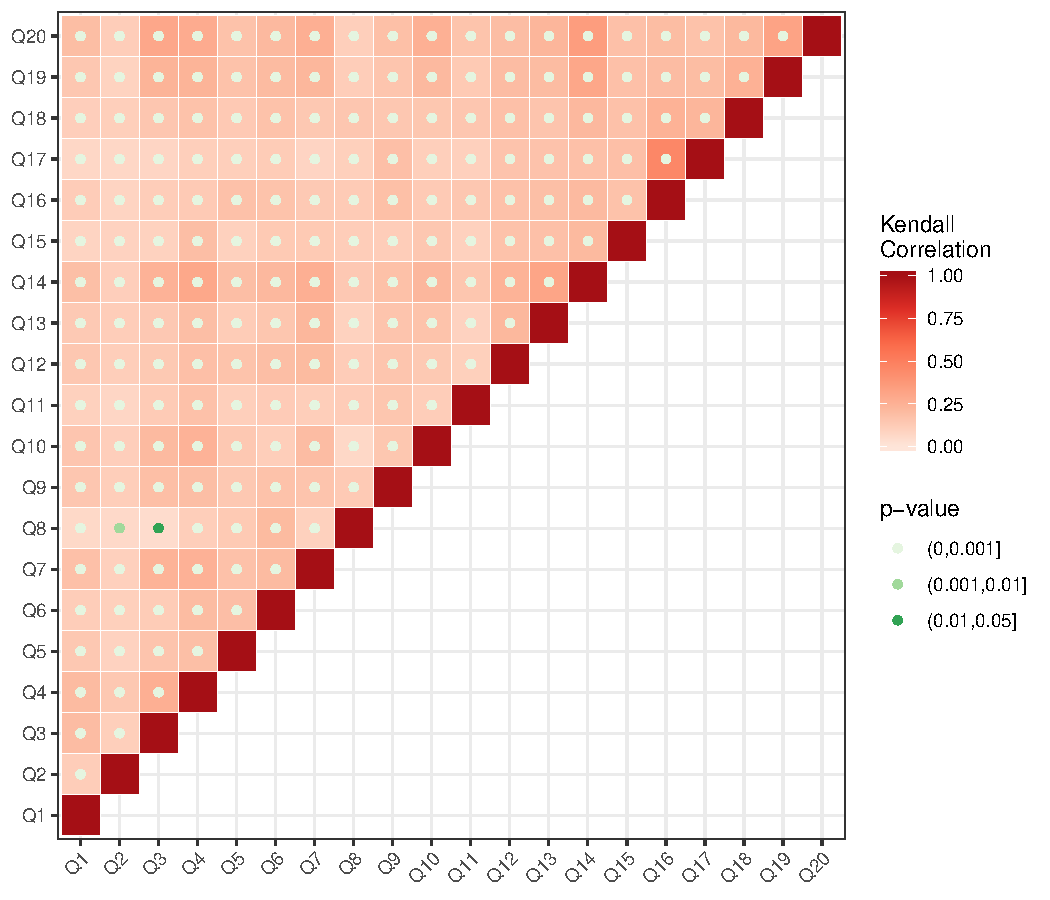
\includegraphics[width=\linewidth]{fig/IRT_cor_pre17.pdf}
  \caption{\label{fig:IRT_cor_pre17}Correlation heat map and significance indicators of the Kendall's $\tau$ test}
\end{figure}

The six largest $p$-values of the significance test are also shown in Table~\ref{tab:IRT_cortest}. All pairs of questions except the pair (Q3, Q8) have $p$-values lower than 0.01, suggesting the null hypotheses are rejected at the 99\% significance level. The null hypothesis of the pair (Q3, Q8) is rejected at the 95\% significance level. Therefore, the assumption of local independence that there is an underlying structure is entitled. 

\begin{table}[ht]
    \centering
    \begin{tabular}{ccc}
      \hline
    Item $i$ & Item $j$ & $p$-values \\ 
    \hline
    Q3 & Q8 & 0.0139 \\ 
      Q2 & Q8 & 0.0015 \\ 
      Q1 & Q8 & 0.0006 \\ 
      Q2 & Q17 & 0.0002 \\ 
      Q8 & Q10 & 0.0002 \\ 
      Q1 & Q17 & 0.0001 \\ 
       \hline
    \end{tabular}
    \caption{\label{tab:IRT_cortest}Four largest $p$-values from Kendall's $\tau$ test}
\end{table}

\section{Dimensionality}

An exploratory factor analysis (EFA) is essential to identify the latent structure of variables (items) and determine the number of latent variables to use in PCM. The \texttt{R} package \texttt{psych} is used in this section. 

A scree plot of the eigenvalues for a principal axis factor analysis, along with the plots of simulated and resampled data are shown in Figure~\ref{fig:EFA_scree}. The eigenvalue of factor number 2 decreases greatly and the eigenvalues start to level off from this point. Besides, the difference between simulated data and actual data is minimised at the point of factor number 6. These suggest that an integer between 1 and 6 would be a good choice for the number of factors to be extracted. 

\begin{figure}[H]
  \centering
  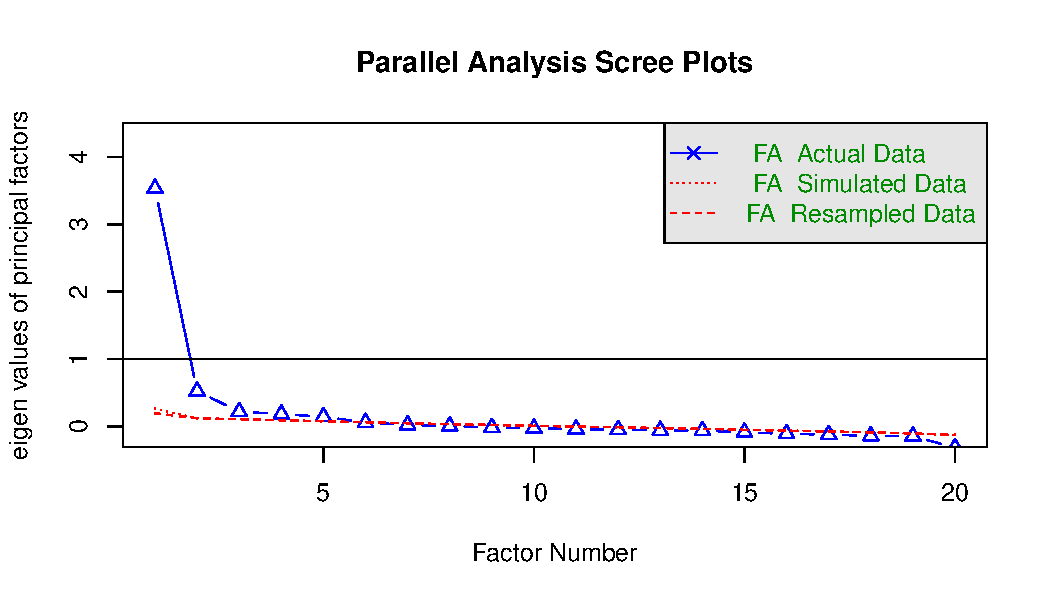
\includegraphics[width=\linewidth]{fig/EFA_scree.pdf}
  \caption{\label{fig:EFA_scree}Parallel analysis scree plots}
\end{figure}

A suitable number of factors should result in a simple structure of factor loadings that the loadings should greater than a given threshold (0.25 is used in this report) and an item should not load on more than one factor. We should also validate the model with simple structure by assessing the Root Mean Square of Residuals (RMSR) which is acceptable when it is close to 0, Root Mean Square Error of Approximation (RMSEA) index which shows a good model fit when it is less than 0.05, and Tucker Lewis Index (TLI) which is acceptable when it is greater than 0.9. 

\subsection{One factor}

We first carry out EFA with one factor using minimum residual as the factoring method and `oblimin' as the oblique transformation of the solution, because of the existence of correlation in the factors \cite{web:efa}. With only one factor, this factor can be interpreted as `general mathematical ability'. 

The standardised loadings on the factors and the indicator of loadings greater or equal to 0.25 are shown in Table~\ref{tab:EFA_pre17_1}. The loadings are also plotted along the Factor 1 axis in Figure~\ref{fig:EFA_pre17_1}. The variable Q2 is not significant though it has the loading of 0.233 on the factor which is slightly lower than 0.25. It should be noted that the loadings of Type-B questions are generally larger than Type-A, indicating that Type-B questions are better measures of higher mathematical ability. 

\begin{table}[ht]
  \begin{minipage}{0.5\linewidth}
    \centering
    \begin{tabular}{lccc}
      \hline
    & Type & MR1 & \\ 
      \hline
    Q1 & A & 0.353 & * \\ 
      Q2 & A & 0.233 &  \\ 
      Q3 & B & 0.421 & * \\ 
      Q4 & A & 0.537 & * \\ 
      Q5 & A & 0.356 & * \\ 
      Q6 & A & 0.405 & * \\ 
      Q7 & B & 0.456 & * \\ 
      Q8 & A & 0.256 & * \\ 
      Q9 & A & 0.378 & * \\ 
      Q10 & B & 0.414 & * \\ 
      \hline
    \end{tabular}
  \end{minipage}%
  \begin{minipage}{0.5\linewidth}
    \centering
    \begin{tabular}{lccc}
      \hline
     & Type & MR1 & \\ 
      \hline
    Q11 & A & 0.309 & * \\ 
      Q12 & A & 0.432 & * \\ 
      Q13 & A & 0.448 & * \\ 
      Q14 & B & 0.608 & * \\ 
      Q15 & A & 0.357 & * \\ 
      Q16 & A & 0.421 & * \\ 
      Q17 & A & 0.366 & * \\ 
      Q18 & A & 0.411 & * \\ 
      Q19 & B & 0.499 & * \\ 
      Q20 & B & 0.550 & * \\ 
       \hline
    \end{tabular}  
  \end{minipage}
  \caption{\label{tab:EFA_pre17_1}Loadings of items on factor where `*' indicates loadings greater or equal to 0.25}
\end{table}

\begin{figure}[H]
  \centering
  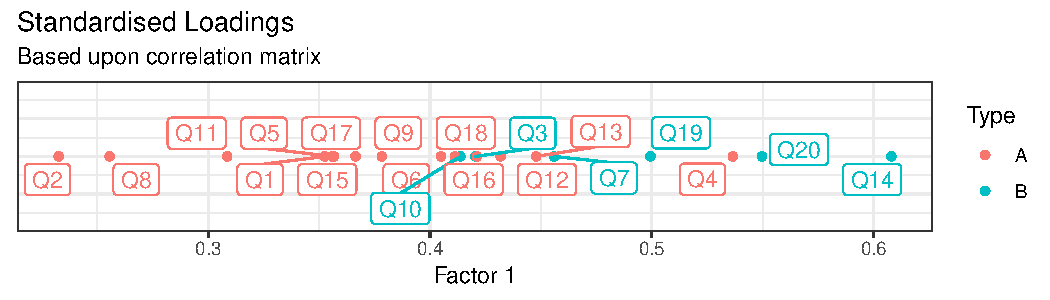
\includegraphics[width=\linewidth]{fig/EFA_pre17_1.pdf}
  \caption{\label{fig:EFA_pre17_1}Standardised loadings on Factor 1}
\end{figure}

The RMSR of this model is 0.04. The 90\% confidence interval of RMSEA index is (0.041, 0.046). The TLI of factoring reliability is 0.859. All these statistics suggest that this EFA with 1 factor is a reasonable fit. 

\subsection{Two factors}

Next, we consider adding an additional factor to EFA to examine whether the results are improved. Table~\ref{tab:EFA_pre17_2} shows the factor loadings which are greater or equal to 0.25 only. In this model, three variables (Q2, Q8 and Q15) become non-significant and one variable (Q18) loads on more than one factor. This violates the simple structure we aim to have that items are only single-loading. 

\begin{table}[ht]
  \begin{minipage}{0.5\linewidth}
    \centering
    \begin{tabular}{lccc}
      \hline
     & Type & MR1 & MR2 \\ 
      \hline
    Q1 & A & 0.386 &  \\ 
      Q2 & A &  &  \\ 
      Q3 & B & 0.512 &  \\ 
      Q4 & A & 0.592 &  \\ 
      Q5 & A & 0.327 &  \\ 
      Q6 & A & 0.360 &  \\ 
      Q7 & B & 0.521 &  \\ 
      Q8 & A &  &  \\ 
      Q9 & A & 0.305 &  \\ 
      Q10 & B & 0.441 &  \\ 
       \hline
    \end{tabular}
  \end{minipage}%
  \begin{minipage}{0.5\linewidth}
    \centering
    \begin{tabular}{lccc}
      \hline
    & Type & MR1 & MR2 \\ 
      \hline
    Q11 & A & 0.258 &  \\ 
      Q12 & A & 0.359 &  \\ 
      Q13 & A & 0.374 &  \\ 
      Q14 & B & 0.588 &  \\ 
      Q15 & A &  &  \\ 
      Q16 & A &  & 0.615 \\ 
      Q17 & A &  & 0.688 \\ 
      Q18 & A & 0.256 & 0.258 \\ 
      Q19 & B & 0.446 &  \\ 
      Q20 & B & 0.557 &  \\ 
      \hline
    \end{tabular}
  \end{minipage}
  \caption{\label{tab:EFA_pre17_2}Loadings of items on factors which are greater or equal to 0.25 only}
\end{table}

Figure~\ref{fig:EFA_pre17_2} is the scatter plot of the standardised loadings on Factor 2 against the standardised loadings on Factor 1. The loadings of Type-B questions are again generally higher than Type-A questions. However, Q4, which is a Type-A question, has the highest loading on Factor 1 among all questions. Q16 and Q17 have high loadings on Factor 2 and low loadings on Factor 1, which are the contrary of the rest of the questions. It is worth noticing that Q16 and Q17 are multiple choice questions and require knowledge of differential calculus. 

\begin{figure}[H]
  \centering
  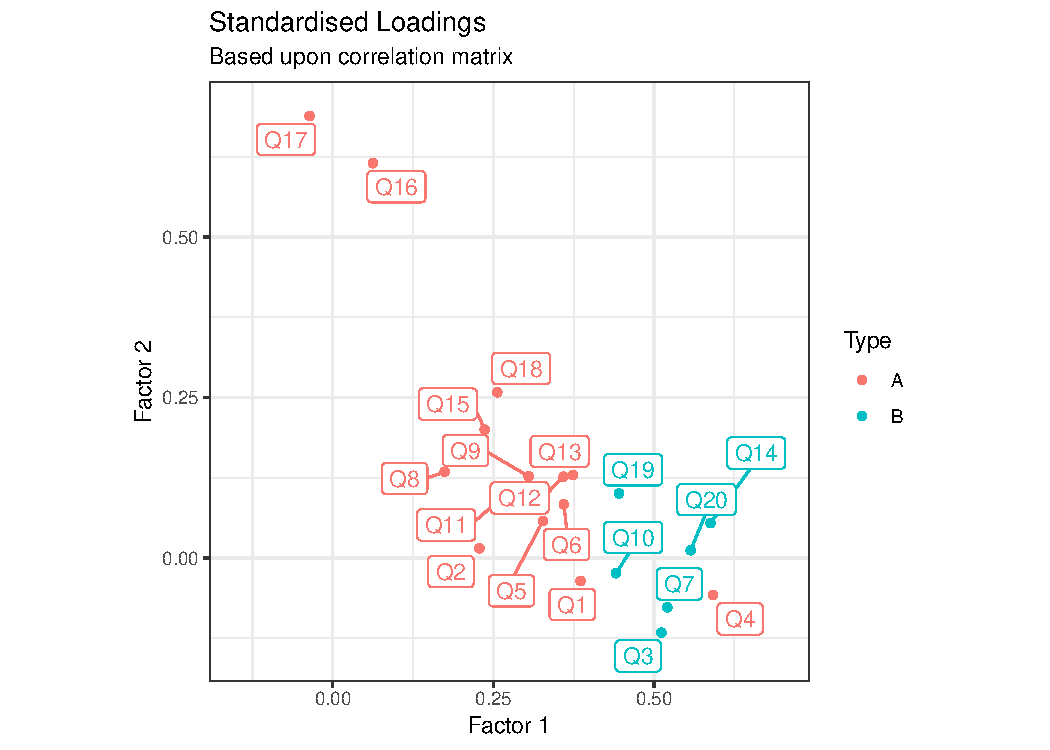
\includegraphics[width=\linewidth]{fig/EFA_pre17_2.pdf}
  \caption{\label{fig:EFA_pre17_2}Standardised loadings on Factor 2 against Factor 1}
\end{figure}

\subsection{More factors}

In addition, EFAs with 3, 4, 5 and 6 factors were also performed. However, the structure of variables of these models were not as simple as the model with only 1 factor and there were not large improvement of the statistics including RMSR, RMSEA and Tucker Lewis Index. 

Considering the results above, as well as the simplicity of interpreting the factors, we proceed with an one-factor structure, i.e. the overall (undivided) mathematical ability. 

\section{Model selection}

A 1PL model, i.e. the model with fixed item slope parameters, is firstly fitted, using the packages \texttt{ltm} \cite{ltm} and \texttt{mirt} \cite{mirt} in \texttt{R}. For reference, we refer to this model as Model \texttt{MDT2-1PL}. The item response curves (i.e. the item expected score functions), test response curve (i.e. the test expected score functions), item information curves and test information curve are shown in Figure~\ref{fig:IRT_pre17_1PL}. 

Based on 200 data sets (including 199 bootstrapped samples), the p-value of the goodness-of-fit test is 0.12, which is non significant, suggesting that the 1PL model is an acceptable fit to the data. In Table~\ref{tab:IRT_pre17_1PL_itemfit} are shown the $S\text{-}X^2$ item-fit statistics and corresponding goodness-of-fit tests on item level. The significance codes are interpreted in the same way as \texttt{R} output, i.e. 

\begin{center}
Signif. codes: 0 ‘***’ 0.001 ‘**’ 0.01 ‘*’ 0.05 ‘.’ 0.1 ‘ ’ 1. 
\end{center}

\noindent
These statistics indicate that 12 of the 20 items are not well represented by the estimated 1PL GPCM item parameters. 

\begin{figure}[H]
  \centering
  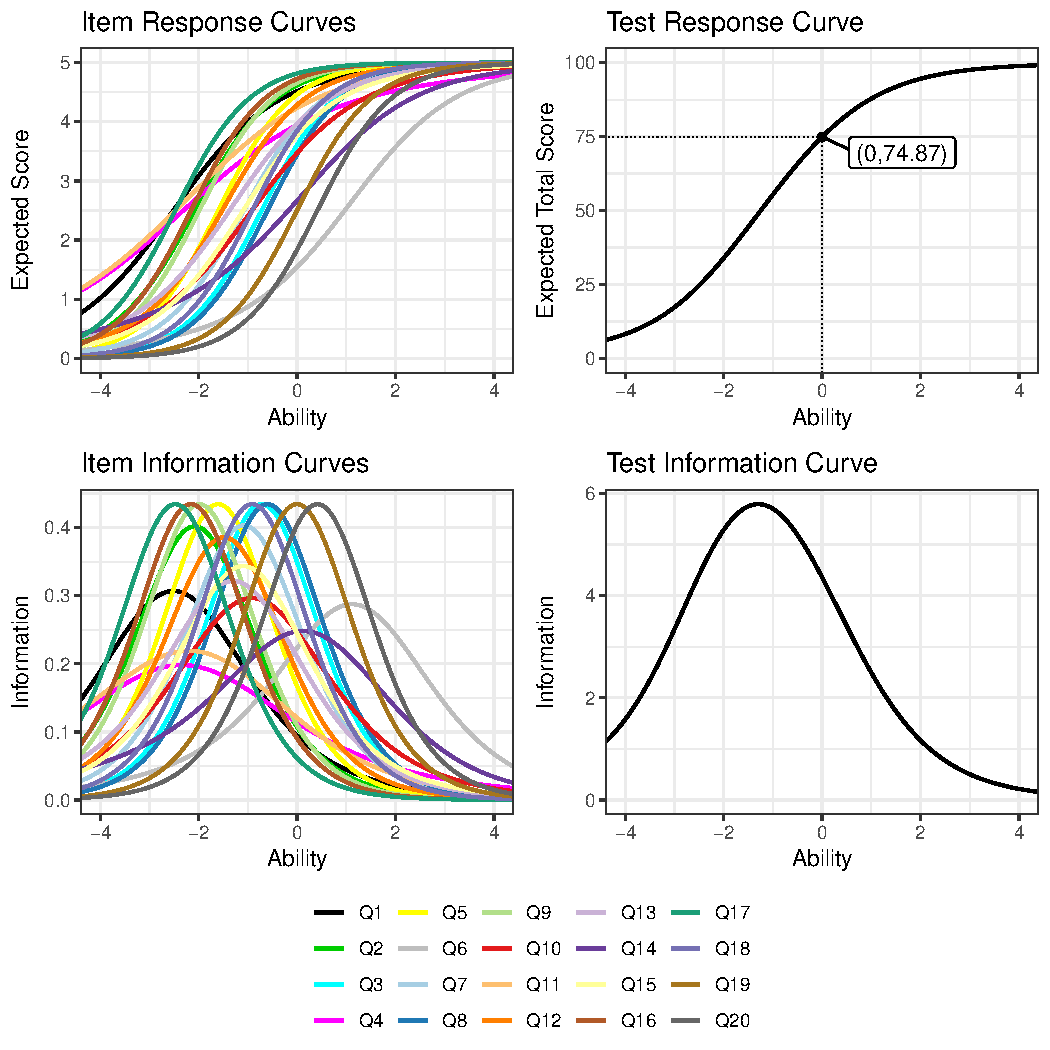
\includegraphics[width=\linewidth]{fig/IRT_pre17_1PL.pdf}
  \caption{\label{fig:IRT_pre17_1PL}Plots of the 1PL model with equal discrimination parameters (Model \texttt{MDT2-1PL})}
\end{figure}

\begin{table}[H]
  \begin{minipage}{0.5\linewidth}
    \centering
    \begin{tabular}{lrrcl}
      \hline
    Item & $S$-$X^2$ & df & p-value & \\ 
      \hline
    Q1 & 79.2 & 72 & 0.262 &  \\ 
      Q2 & 139.9 & 66 & 0.000 & *** \\ 
      Q3 & 84.1 & 37 & 0.000 & *** \\ 
      Q4 & 352.8 & 206 & 0.000 & *** \\ 
      Q5 & 61.3 & 37 & 0.007 & ** \\ 
      Q6 & 109.2 & 67 & 0.001 & *** \\ 
      Q7 & 74.2 & 65 & 0.204 &  \\ 
      Q8 & 293.4 & 36 & 0.000 & *** \\ 
      Q9 & 32.5 & 38 & 0.723 &  \\ 
      Q10 & 75.4 & 70 & 0.308 &  \\ 
       \hline
    \end{tabular}
  \end{minipage}%
  \begin{minipage}{0.5\linewidth}
    \centering
    \begin{tabular}{lrrcl}
      \hline
    Item & $S$-$X^2$ & df & p-value & \\ 
      \hline
    Q11 & 139.8 & 114 & 0.051 & . \\ 
      Q12 & 123.4 & 90 & 0.011 & * \\ 
      Q13 & 119.2 & 89 & 0.018 & * \\ 
      Q14 & 236.1 & 110 & 0.000 & *** \\ 
      Q15 & 284.9 & 110 & 0.000 & *** \\ 
      Q16 & 38.7 & 37 & 0.392 &  \\ 
      Q17 & 31.4 & 37 & 0.726 &  \\ 
      Q18 & 74.8 & 37 & 0.000 & *** \\ 
      Q19 & 38.0 & 34 & 0.292 &  \\ 
      Q20 & 57.3 & 32 & 0.004 & ** \\ 
       \hline
    \end{tabular}
  \end{minipage}
  \caption{\label{tab:IRT_pre17_1PL_itemfit}Item-fit statistics for Model \texttt{MDT2-1PL} using $S\text{-}X^2$ statistics}
\end{table}

Based on the finding from the report last year, which used binary scoring, a model with different discrimination parameters provides a better fit to the data than a model with fixed discrimination parameters. A 1PL model is therefore not expected to be a good fit because of the large variation in the discrimination parameters estimated by the 2-parameter dichotomous model. 

An unconstrained GPCM (Model \texttt{MDT2-GPCM}) is fitted in the next step. The item response curves, test response curve, item information curves and test information curve are shown in Figure~\ref{fig:IRT_pre17_GPCM}. 

\begin{figure}[H]
  \centering
  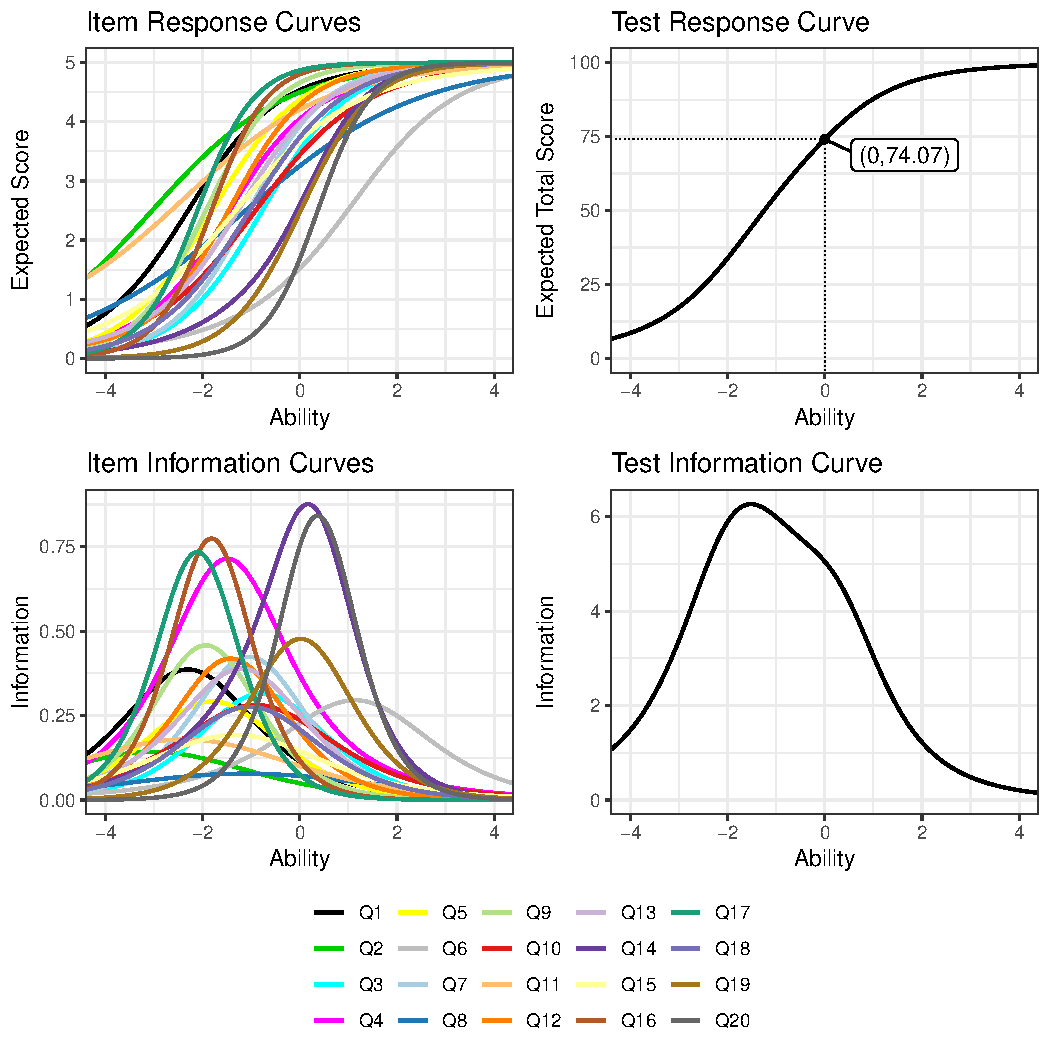
\includegraphics[width=\linewidth]{fig/IRT_pre17_GPCM.pdf}
  \caption{\label{fig:IRT_pre17_GPCM}Plots of the unconstrained GPCM (Model \texttt{MDT2-GPCM})}
\end{figure}

\begin{table}[H]
  \begin{minipage}{0.5\linewidth}
    \centering
    \begin{tabular}{lrrcl}
      \hline
      Item & $S$-$X^2$ & df & p-value & \\ 
      \hline
    Q1 & 74.8 & 71 & 0.355 &  \\ 
      Q2 & 81.3 & 69 & 0.147 &  \\ 
      Q3 & 58.3 & 37 & 0.014 & * \\ 
      Q4 & 230.3 & 186 & 0.015 & * \\ 
      Q5 & 43.1 & 39 & 0.300 &  \\ 
      Q6 & 101.7 & 68 & 0.005 & ** \\ 
      Q7 & 69.7 & 65 & 0.321 &  \\ 
      Q8 & 31.7 & 39 & 0.791 &  \\ 
      Q9 & 32.1 & 38 & 0.740 &  \\ 
      Q10 & 68.8 & 70 & 0.517 &  \\ 
       \hline
    \end{tabular}
  \end{minipage}%
  \begin{minipage}{0.5\linewidth}
    \centering
    \begin{tabular}{lrrcl}
      \hline
      Item & $S$-$X^2$ & df & p-value & \\
      \hline
    Q11 & 129.1 & 115 & 0.174 &  \\ 
      Q12 & 123.4 & 90 & 0.011 & * \\ 
      Q13 & 120.4 & 90 & 0.018 & * \\ 
      Q14 & 127.9 & 102 & 0.043 & * \\ 
      Q15 & 214.3 & 120 & 0.000 & *** \\ 
      Q16 & 45.9 & 36 & 0.124 &  \\ 
      Q17 & 36.0 & 35 & 0.420 &  \\ 
      Q18 & 36.3 & 37 & 0.503 &  \\ 
      Q19 & 38.5 & 34 & 0.271 &  \\ 
      Q20 & 40.6 & 30 & 0.093 & . \\ 
       \hline
    \end{tabular}
  \end{minipage}
  \caption{\label{tab:IRT_pre17_GPCM_itemfit}Item-fit statistics for Model \texttt{MDT2-GPCM} using $S\text{-}X^2$ statistics}
\end{table}

Based on 200 data sets (including 199 bootstrapped samples), the p-value of the goodness-of-fit test is 0.14, suggesting an acceptable fit of the model. The $S\text{-}X^2$ item-fit statistics and corresponding goodness-of-fit tests on item level are shown in Table~\ref{tab:IRT_pre17_GPCM_itemfit}. There are 7 of the 20 items which are not well represented by the estimated GPCM item parameters. 

The likelihood ratio (LR) test statistics are shown in Table~\ref{tab:IRT_anova}. The $p$-value suggests the null hypothesis (that item slope parameters $a_i = 0$) is rejected at the 99\% significance level, which means that the GPCM is a significant improvement over the 1PL model. In Table~\ref{tab:IRT_anova} are also shown the AIC values and other kinds of information criterion used for model selection. The AIC of GPCM is 92414, which is less than the AIC of 1PL model, though the number of parameters increased by 19. 

\begin{table}[ht]
  \centering
  \begin{tabular}{cccccccccc}
    \hline
Model & AIC & AICc & SABIC & HQ & BIC & logLik & $\lambda$ & df & p \\ 
  \hline
\texttt{MDT2-1PL} & 93133 & 93135 & 93278 & 93242 & 93437 & -46516 &  &  &  \\ 
  \texttt{MDT2-GPCM} & 92414 & 92417 & 92614 & 92564 & 92834 & -46138 & 757 & 19 & 0.0000 \\ 
   \hline
  \end{tabular}
  \caption{\label{tab:IRT_anova}Model selection table with likelihood ratio test and AIC comparison}
\end{table}

Since all the statistics suggests that Model \texttt{MDT2-GPCM} is a better fit to the data than Model \texttt{MDT2-1PL}, we proceed with Model \texttt{MDT2-GPCM}. 

\section{GPCM}

\subsection{Difficulty and discrimination}

When comparing the discriminations and difficulties of the items, the estimations of the coefficients cannot be used directly, because the definitions of the parameters in polytomous IRT models are different from the way they are in dichotomous IRT models \cite{IRT}. The discrimination of an item depends on the slope parameter $a_i$ and the relative difficulties between consecutive categories $\delta_{ic}$. Alternatively, these characteristics can be accessed from the expected scores $\bar T_i(\theta)$ given a sequence of ability values. 

In Table~\ref{tab:IRT_pre17_expscore} are shown the expected scores of the students with average ability ($\theta=0$) and the changes of the expectations of the students within two standard deviations of the mean, i.e. $\theta = \pm 2$. Since the ability $\theta$ follows a standard normal distribution, this range of ability covers 95.4\% of students. The column `Facility' shows the expected scores of students average ability. The final column shows the difference in expected scores between the most and least able students, and thus we use this as a measure of discrimination. 

\begin{table}[H]
  \centering
  \begin{tabular}{ccccc}
    \hline
   & $\bar T_i (-2) - \bar T_i (0)$ & Facility & $\bar T_i (2) - \bar T_i (0)$ & Discrimination\\ 
   \hline
  Q1 & -1.65 & 4.53 & 0.37 & 2.02 \\ 
    Q2 & -1.09 & 4.49 & 0.36 & 1.46 \\ 
    Q3 & -2.52 & 3.52 & 1.27 & 3.78 \\ 
    Q4 & -2.27 & 4.05 & 0.71 & 2.99 \\ 
    Q5 & -2.14 & 4.37 & 0.54 & 2.69 \\ 
    Q6 & -1.04 & 1.52 & 2.05 & 3.09 \\ 
    Q7 & -2.77 & 3.93 & 0.94 & 3.71 \\ 
    Q8 & -1.36 & 3.25 & 1.00 & 2.36 \\ 
    Q9 & -2.27 & 4.66 & 0.32 & 2.59 \\ 
    Q10 & -2.05 & 3.44 & 1.15 & 3.20 \\ 
    Q11 & -1.22 & 4.21 & 0.54 & 1.76 \\ 
    Q12 & -2.57 & 4.29 & 0.62 & 3.19 \\ 
    Q13 & -2.40 & 3.98 & 0.86 & 3.25 \\ 
    Q14 & -1.98 & 2.59 & 2.17 & 4.15 \\ 
    Q15 & -1.83 & 3.68 & 0.92 & 2.76 \\ 
    Q16 & -2.71 & 4.80 & 0.19 & 2.90 \\ 
    Q17 & -2.14 & 4.87 & 0.13 & 2.27 \\ 
    Q18 & -2.41 & 3.73 & 1.07 & 3.48 \\ 
    Q19 & -2.18 & 2.46 & 2.23 & 4.41 \\ 
    Q20 & -1.62 & 1.68 & 3.08 & 4.70 \\ 
    \hline
    Sum & -40.21 & 74.07 & 20.53 & 60.75 \\ 
     \hline
  \end{tabular}
  \caption{\label{tab:IRT_pre17_expscore}Expected scores of students with ability -2, 0 and 2}
\end{table}

Using this measure, it can be observed that Q20 is the most discriminating question (with discrimination 4.70) for most students, followed by Q19 (with discrimination 4.41). The least discriminating questions are Q2 ( with discrimination 1.46) and Q11 (with discrimination 1.76); in addition, these items have high expected scores for students of mean ability (4.49 and 4.21 respectively), indicating that the expected scores for most of the students in these two questions are greater than 3. This is consistent with the observed proportions of the scores of students (Table~\ref{tab:IRT_pre17_scoreprop}), where a majority of students scored more than 2.5 or even 5 marks. 

\begin{table}[ht]
  \centering
  \begin{tabular}{rrrrrr}
    \hline
    & \multicolumn{5}{c}{Proportion of scores (\%)} \\
    \cline{2-6}
   & 0 & 1.25 & 2.5 & 3.75 & 5 \\ 
    \hline
  Q2 & 9.8 & - & 3.9 & - & 86.3 \\ 
    Q11 & 3.2 & 4.4 & 21.0 & 1.3 & 70.1 \\ 
    Q19 & 50.1 & - & - & - & 49.9 \\ 
    Q20 & 60.2 & - & - & - & 39.8 \\ 
     \hline
  \end{tabular}
  \caption{\label{tab:IRT_pre17_scoreprop}Proportions of the scores of the students in Q2, Q11 Q19 and Q20}
\end{table}

\subsection{Item information}

One of the purposes of fitting IRT models is to estimate the mathematical ability of a student. In order to have accurate estimations, the item information as well as the test information need to be investigated. In addition to the item information curves and test information curves plotted in Figure~\ref{fig:IRT_pre17_GPCM}, a plot of stacked item information curves is shown in Figure~\ref{fig:IRT_pre17_GPCM_stackinfo}. 

% \begin{figure}[H]
%   \centering
%   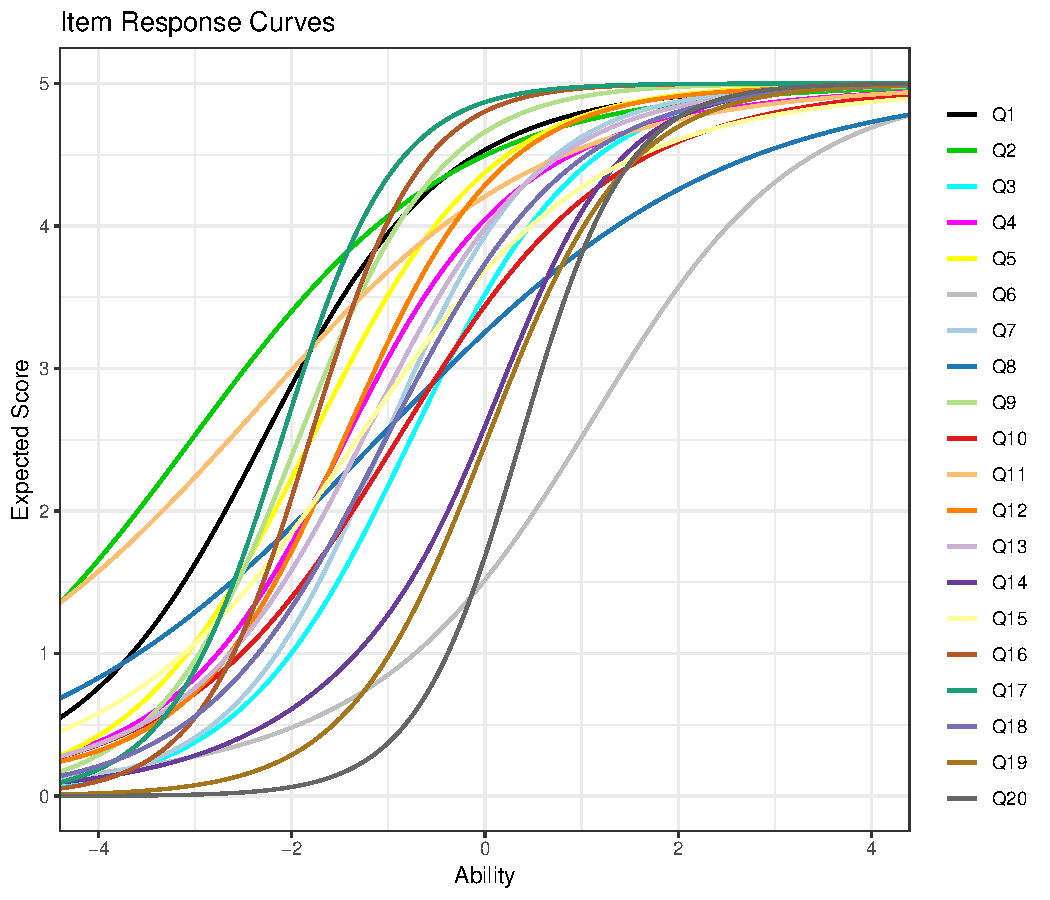
\includegraphics[width=\linewidth]{fig/IRT_pre17_GPCM_irf.pdf}
%   \caption{\label{fig:IRT_pre17_GPCM_irf}Plot of item information curves for the generalised partial credit model}
% \end{figure}

% \begin{figure}[H]
%   \centering
%   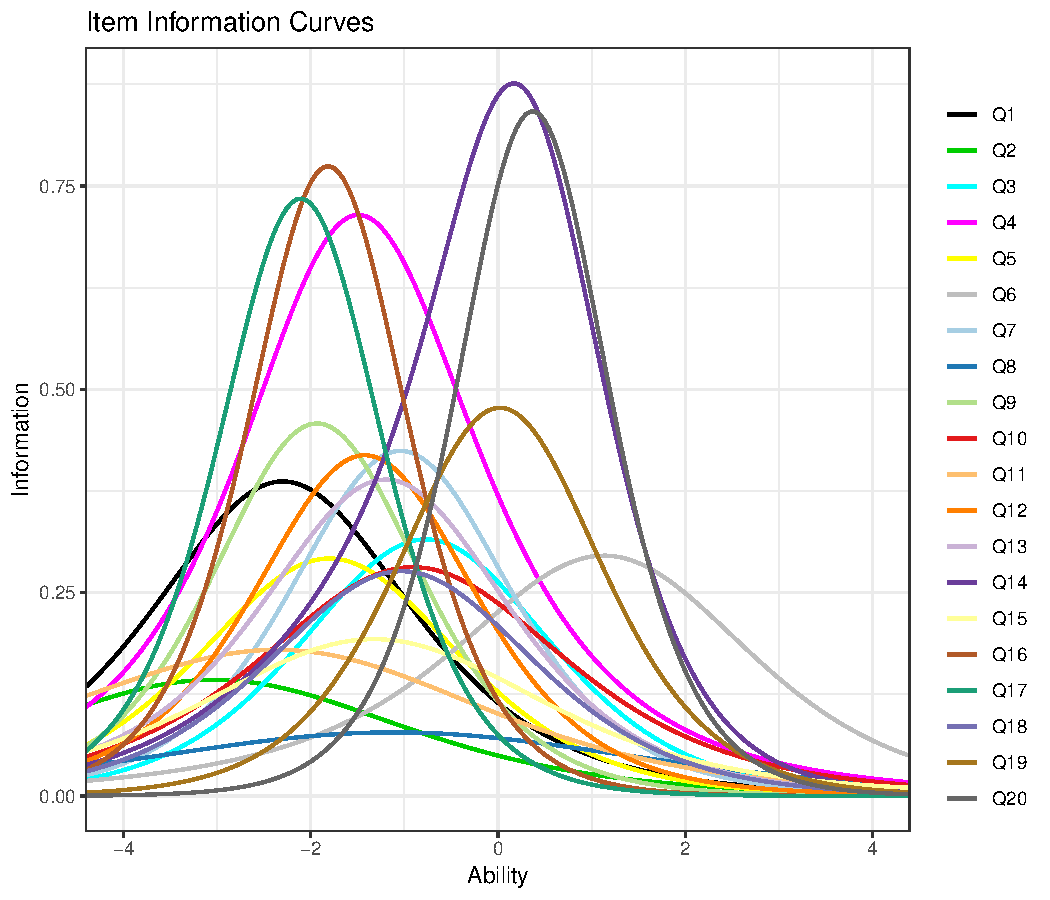
\includegraphics[width=\linewidth]{fig/IRT_pre17_GPCM_info.pdf}
%   \caption{\label{fig:IRT_pre17_GPCM_info}Plot of item information curves for the generalised partial credit model}
% \end{figure}

\begin{figure}[H]
  \centering
  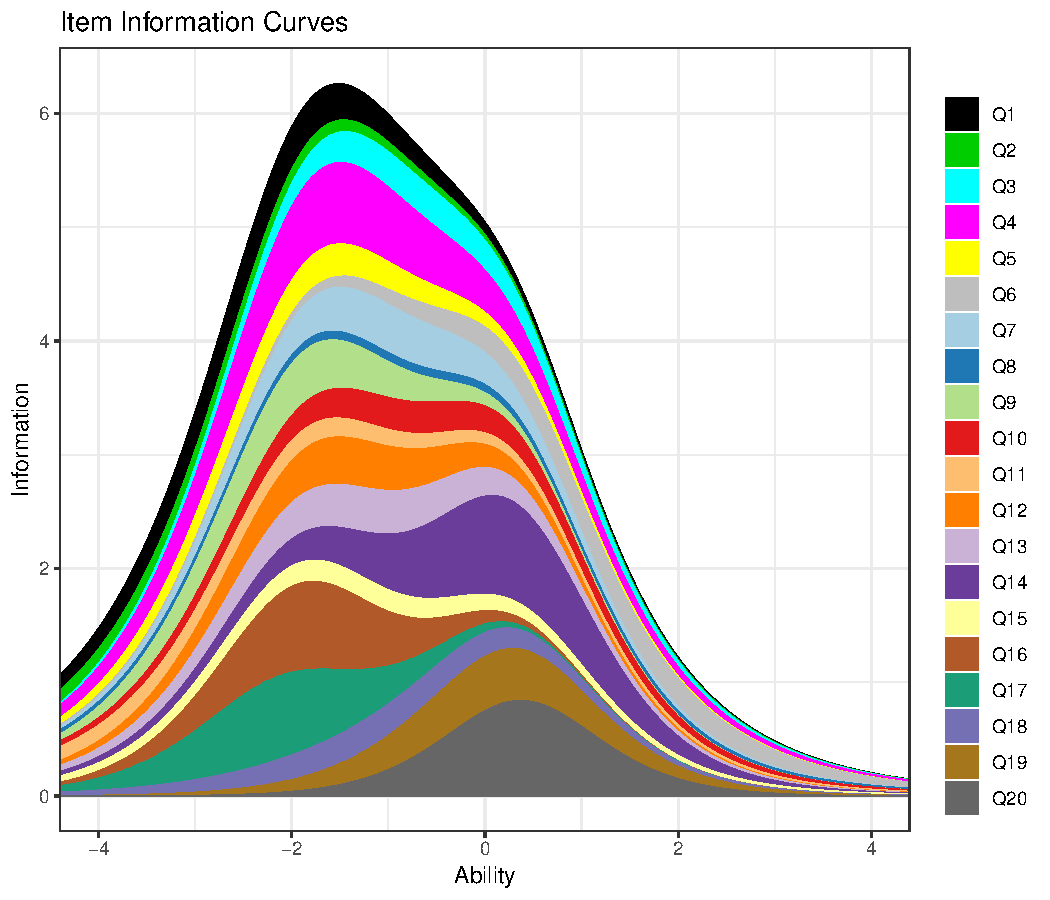
\includegraphics[width=\linewidth]{fig/IRT_pre17_GPCM_stackinfo.pdf}
  \caption{\label{fig:IRT_pre17_GPCM_stackinfo}Plot of stacked item information curves for Model \texttt{MDT2-GPCM}}
\end{figure}

From the figure and Table~\ref{tab:IRT_pre17_summaryiif}, we see that the test information function attains its maximum at $\theta=-1.52$. The area under the test information curves over the range of negative ability is greater than the information area over the positive ability. We also consider restricting the range of integration to $(-2,2)$ (i.e. representing 95.4\%) of students), shown as `Major Info Area' in Table~\ref{tab:IRT_pre17_summaryiif}. % Even if I restrict the range of integration to be computed to $(-2,2)$ (i.e. representing 95.4\% of students), the information area of the below-average students is still twice as large as the area of the above-average students, which are shown as `Major Info Area' in Table~\ref{tab:IRT_pre17_summarytif}. 

From the overall test information shown at the end of Table~\ref{tab:IRT_pre17_summaryiif}, we see that the information area of the below-average students is still twice as large as the area of the above-average students. This indicates that when estimating the abilities of the examinees, the accuracy of measuring above-average students is relatively lower. 

% \begin{table}[ht]
%   \centering
%   \begin{tabular}{rr|rrr|rrr}
%     \hline
%     & & \multicolumn{3}{c|}{Major Info Area} & \multicolumn{3}{c}{Total Info Area} \\
%    & Max at & Lower & Upper & Total & Lower & Upper & Total \\ 
%     \hline
%   Test Information & -1.52 & 11.70 & 6.19 & 17.89 & 20.77 & 7.60 & 28.37 \\ 
%      \hline
%   \end{tabular}
%   \caption{\label{tab:IRT_pre17_summarytif}The area under the test information curve of Model PRE17-GPCM over different definite integral ranges}
% \end{table}

The values of ability where the item information functions attain their maximum are also shown in Table~\ref{tab:IRT_pre17_summaryiif}. Only 4 of the 20 items have their maximum at positive ability values, which is one of the contributing factors leading to the negative skew of the test information curve. 

\begin{table}[H]
  \centering
  \begin{tabular}{rr|rrr|rrr}
    \hline
    & & \multicolumn{3}{c|}{Major Info Area} & \multicolumn{3}{c}{Total Info Area} \\
   & Max at & Lower & Upper & Total & Lower & Upper & Total \\ 
   \hline
   Q1 & -2.30 & 0.49 & 0.11 & 0.60 & 1.35 & 0.14 & 1.49 \\ 
     Q2 & -3.04 & 0.17 & 0.06 & 0.23 & 0.70 & 0.08 & 0.78 \\ 
     Q3 & -0.77 & 0.57 & 0.28 & 0.85 & 0.79 & 0.33 & 1.12 \\ 
     Q4 & -1.49 & 1.21 & 0.38 & 1.59 & 2.15 & 0.51 & 2.66 \\ 
     Q5 & -1.80 & 0.46 & 0.12 & 0.58 & 0.95 & 0.14 & 1.08 \\ 
     Q6 & 1.13 & 0.28 & 0.55 & 0.83 & 0.41 & 0.93 & 1.34 \\ 
     Q7 & -1.04 & 0.75 & 0.26 & 1.00 & 1.06 & 0.29 & 1.35 \\ 
     Q8 & -1.11 & 0.15 & 0.11 & 0.26 & 0.36 & 0.20 & 0.56 \\ 
     Q9 & -1.93 & 0.62 & 0.09 & 0.70 & 1.26 & 0.09 & 1.35 \\ 
     Q10 & -0.91 & 0.52 & 0.30 & 0.82 & 0.88 & 0.40 & 1.28 \\ 
     Q11 & -2.36 & 0.29 & 0.13 & 0.42 & 1.00 & 0.19 & 1.19 \\ 
     Q12 & -1.42 & 0.71 & 0.17 & 0.88 & 1.18 & 0.20 & 1.37 \\ 
     Q13 & -1.20 & 0.70 & 0.25 & 0.95 & 1.16 & 0.30 & 1.46 \\ 
     Q14 & 0.17 & 1.03 & 1.13 & 2.17 & 1.35 & 1.26 & 2.61 \\ 
     Q15 & -1.32 & 0.36 & 0.18 & 0.54 & 0.72 & 0.26 & 0.98 \\ 
     Q16 & -1.81 & 0.95 & 0.07 & 1.02 & 1.69 & 0.07 & 1.76 \\ 
     Q17 & -2.11 & 0.73 & 0.04 & 0.78 & 1.67 & 0.05 & 1.71 \\ 
     Q18 & -1.03 & 0.51 & 0.22 & 0.73 & 0.79 & 0.27 & 1.05 \\ 
     Q19 & 0.02 & 0.60 & 0.62 & 1.22 & 0.68 & 0.70 & 1.38 \\ 
     Q20 & 0.37 & 0.59 & 1.13 & 1.72 & 0.62 & 1.22 & 1.84 \\ 
      \hline
    Test & -1.52 & 11.70 & 6.19 & 17.89 & 20.77 & 7.60 & 28.37 \\ 
     \hline
  \end{tabular}
  \caption{\label{tab:IRT_pre17_summaryiif}The area under each item information curve over different definite integral ranges}
\end{table}

Table~\ref{tab:IRT_pre17_info} shows the Major Info Area and Total Info Area of each item, ordered by the proportion of the total area. In terms of total item information, Q4 and Q14 have the largest areas and each of them accounts for more than 9\% of the total information area, while Q8 and Q2 have the smallest areas and each accounts for less than 3\% of the total information area. As shown in Figure~\ref{fig:IRT_pre17_GPCM_stackinfo}, the area over the range of $\theta<2$ occupies a large proportion of the total information, but there are only 2.3\% of students with abilities which are lower than -2, according to the prior belief that the distribution of ability is Standard Normal Distribution $N(0,1)$. Therefore, comparing the information area over the range from -2 to 2 is much more meaningful than comparing the area over than whole range of ability. 

In terms of major item information, Q2 and Q8 are still the least informative but with even lower proportion of the total information area of the 20 items. Q11 becomes the third least informative item, with 2.33\% of the total information area. On the other hand, Q14 becomes the most informative item and accounts for over 12\% of the total information. It should also be noted that Type-B questions are generally more informative than Type-A questions. The rank of the major information areas of the items is similar to the rank of the loadings on a one-factor factor analysis model, which is shown in Figure~\ref{fig:EFA_pre17_1}.  

\begin{table}[H]
  \begin{minipage}{0.5\linewidth}
      \centering
      \begin{tabular}{lcrr}
        \hline
      Item & Type & MajorInfo & Prop (\%) \\ 
        \hline
      Q2 & A & 0.23 & 1.28 \\ 
        Q8 & A & 0.26 & 1.48 \\ 
        Q11 & A & 0.42 & 2.33 \\ 
        Q15 & A & 0.54 & 3.02 \\ 
        Q5 & A & 0.58 & 3.25 \\ 
        Q1 & A & 0.60 & 3.37 \\ 
        Q9 & A & 0.70 & 3.92 \\ 
        Q18 & A & 0.73 & 4.09 \\ 
        Q17 & A & 0.78 & 4.35 \\ 
        Q10 & B & 0.82 & 4.58 \\ 
        Q6 & A & 0.83 & 4.62 \\ 
        Q3 & B & 0.85 & 4.75 \\ 
        Q12 & A & 0.88 & 4.90 \\ 
        Q13 & A & 0.95 & 5.29 \\ 
        Q7 & B & 1.00 & 5.62 \\ 
        Q16 & A & 1.02 & 5.71 \\ 
        Q19 & B & 1.22 & 6.81 \\ 
        Q4 & A & 1.59 & 8.88 \\ 
        Q20 & B & 1.72 & 9.64 \\ 
        Q14 & B & 2.17 & 12.11 \\ 
         \hline
      \end{tabular}
  \end{minipage}%
  \begin{minipage}{0.5\linewidth}
    \centering
    \begin{tabular}{lcrr}
      \hline
    Item & Type & TotalInfo & Prop (\%) \\ 
      \hline
    Q8 & A & 0.56 & 1.97 \\ 
      Q2 & A & 0.78 & 2.76 \\ 
      Q15 & A & 0.98 & 3.46 \\ 
      Q18 & A & 1.05 & 3.71 \\ 
      Q5 & A & 1.08 & 3.81 \\ 
      Q3 & B & 1.12 & 3.96 \\ 
      Q11 & A & 1.19 & 4.18 \\ 
      Q10 & B & 1.28 & 4.52 \\ 
      Q6 & A & 1.34 & 4.71 \\ 
      Q7 & B & 1.35 & 4.77 \\ 
      Q9 & A & 1.35 & 4.77 \\ 
      Q12 & A & 1.37 & 4.84 \\ 
      Q19 & B & 1.38 & 4.87 \\ 
      Q13 & A & 1.46 & 5.13 \\ 
      Q1 & A & 1.49 & 5.25 \\ 
      Q17 & A & 1.71 & 6.04 \\ 
      Q16 & A & 1.76 & 6.20 \\ 
      Q20 & B & 1.84 & 6.47 \\ 
      Q14 & B & 2.61 & 9.20 \\ 
      Q4 & A & 2.66 & 9.37 \\ 
      \hline
    \end{tabular}
  \end{minipage}
  \caption{\label{tab:IRT_pre17_info}Tables of item information as percentage of total information for Model \texttt{MDT2-GPCM} ordered by proportion}
\end{table}

\subsection{\label{sec:IRT_EAP}Ability estimates}

The scatter plot of the actual MDT scores of the students against their estimated abilities (EAP) is shown in Figure~\ref{fig:IRT_pre17_EAP}, along with the corresponding 95\% confidence interval of the estimates. The EAP is computed using their responses to each question. Additionally, the test response curve, i.e. the expected total score given ability, is also plotted in the figure for comparison. 

It is worth noticing that 76 students scored full marks in the test and their abilities are estimated at 1.86. However, there should not exist a upper limit of the ability in the real world. The upper limit of the questions (5 marks each) and the test (100 marks) restricted students with higher abilities from scoring higher and different marks. This may cause a problem when estimating abilities and may skew the shape of the scatter plot. 

\begin{figure}[H]
  \centering
  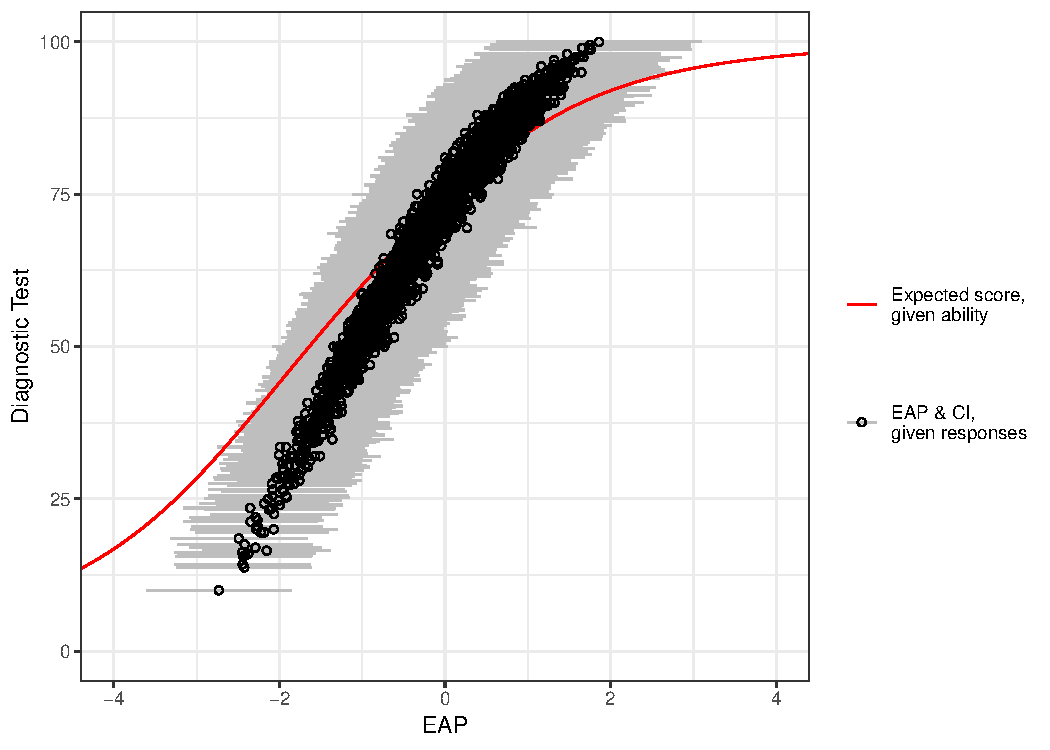
\includegraphics[width=\linewidth]{fig/IRT_pre17_EAP.pdf}
  \caption{\label{fig:IRT_pre17_EAP}Scatter plot of actual MDT scores against EAP and CI, and test response curve}
\end{figure}

\subsection{Comparison with dichotomous model}

The difficulties and the discriminations estimated by Model \texttt{MDT2-GPCM}, a polytomous IRT model, are quite different from the estimates given by the dichotomous models performed last year. 

However, our findings are consistent with the previous recommendation to remove Q2, Q8 and Q11. From the total information area in Table~\ref{tab:IRT_pre17_info} and the information areas for below-average and above-average students respectively in Table~\ref{tab:IRT_pre17_summaryiif}, these three items cannot give relatively higher standard error of measuring the ability of a student and have the highest accuracy only when measuring the students with abilities lower than -2. 

\section{Academic growth}

The academic growth of students from different administrations is always of interest to the examiner. When the entry requirements increase, there would be an upward trend in the abilities of students. In the meantime, the examiner should fine-tune the MDT to address the growth of abilities. 

Since all the questions in MDT2 remained unchanged in years 2013 through 2016, it is possible to calibrate the data from a specific year in an IRT model and use its parameters to estimate the abilities of the students taking MDT2 in other years directly from these fixed item parameters. This procedure will place all the students on the same scale of ability. 

Choosing the year 2013 as the pivot should be the most proper way, but we need each response to be observed at least once, and this was only the case in 2014. I therefore choose the year 2014 as the pivot and fit the GPCM to it. 

The density plot of the estimated abilities of the students using the method of EAP \cite{irtequating} are shown in Figure~\ref{fig:GRTH_density}, where a trend that the distribution shifts to the right as the years go by can be seen. It should be noted that the density plots are not symmetric with a steeper slope on the right hand side. This may due to the existence of the upper limit of the test scores. 

\begin{figure}[H]
  \centering
  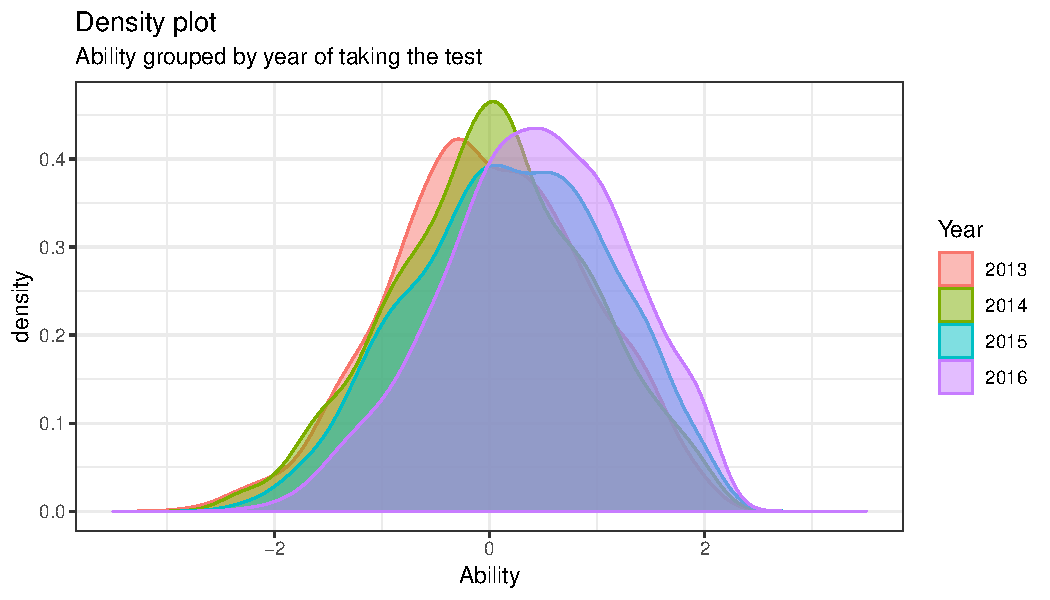
\includegraphics[width=\linewidth]{fig/GRTH_density.pdf}
  \caption{\label{fig:GRTH_density}Density plot of the expected abilities of students grouped by year of taking the test}
\end{figure}

In Table~\ref{tab:GRTH_dsc} are shown the basic descriptive statistics of the distributions of the estimated abilities. 

\begin{table}[ht]
  \centering
  \begin{tabular}{rrrrrrrr}
    \hline
   & n & mean & sd & min & max & skew & kurtosis \\ 
    \hline
  2013 & 832 & -0.01 & 0.90 & -2.75 & 1.97 & -0.09 & -0.37 \\ 
    * 2014 & 942 & 0.02 & 0.90 & -2.37 & 1.97 & -0.08 & -0.35 \\ 
    2015 & 729 & 0.20 & 0.90 & -2.28 & 1.97 & -0.15 & -0.59 \\ 
    2016 & 763 & 0.41 & 0.85 & -2.19 & 1.97 & -0.23 & -0.41 \\ 
     \hline
  \end{tabular}
  \caption{\label{tab:GRTH_dsc}Basic descriptive statistics of the distributions of the estimated abilities (* indicates the pivot test)}
\end{table}

The two-sample Kolmogorov-Smirnov (K-S) test is a nonparametric test comparing the empirical distribution functions of two samples and testing the null hypothesis that the two samples are drawn from the same distributions. This test can be used for examining the changes in both location and shape of the distributions of the estimated abilities. 

In Table~\ref{tab:GRTH_ks} are shown the two-sample K-S test statistics and p-values of the data from consecutive years. The non-significant p-value of the test on the data in 2013 and 2014 suggests students from these two years are drawn from the same distribution of ability, while there are significant differences between students from 2014 and 2015, and between students from 2015 and 2016. 

\begin{table}[ht]
  \centering
  \begin{tabular}{rrr}
    \hline
   & statistic & $p$-value \\ 
    \hline
  2013 vs 2014 & 0.0542 & 0.1498 \\ 
    2014 vs 2015 & 0.1124 & 0.0001 \\ 
    2015 vs 2016 & 0.1107 & 0.0002 \\ 
     \hline
  \end{tabular}
  \caption{\label{tab:GRTH_ks}Kolmogorov-Smirnov test statistics and p-values of the data from consecutive years}
\end{table}

% subset


\chapter{Evaluating MDT3}

An important objective of this project is to evaluate the performance of the new MDT (MDT3) with different questions based on the suggestions from the report last year. 

\section{Approaches to test equating}

A key step in assessing academic growth is test equating, which ensures that all students are placed on a same scale of ability. There are three approaches to IRT equating \cite{irtequating}: 

\begin{enumerate}
\item Separate calibration with linear transformation, which determines the linear relationship between the difficulty parameters in consecutive years. 
\item Fixed common item parameter (FCIP) calibration, which fixes the parameters of the equating items so that these parameters are not estimated in the calibration's future years and remain unchanged, resulting in placing all item parameters on a common metric. 
\item Concurrent parameter calibration, where the data for all years are calibrated together in one IRT model. 
\end{enumerate}

In this chapter, all these three approaches are used and the performances of these test equating approaches are evaluated. 

\section{Testing of assumptions}

Before IRT models are fitted and tests are equated, the assumptions of local independence and dimensionality need to be checked as they are in Chapter~\ref{chap:PCM_pre17}. 

\subsection{Local independence}

The Kendall correlation and the significance indicators of the Kendall' $\tau$ test performed on each pair of items are shown in Figure~\ref{fig:IMPRV_cor_17}. It is shown in the figure that the correlation between any pair of questions are positive. The null hypotheses that the questions in each pair are statistically independent are rejected at 95\% significant level, except the pair (Q1, Q15). 

\begin{figure}[H]
  \centering
  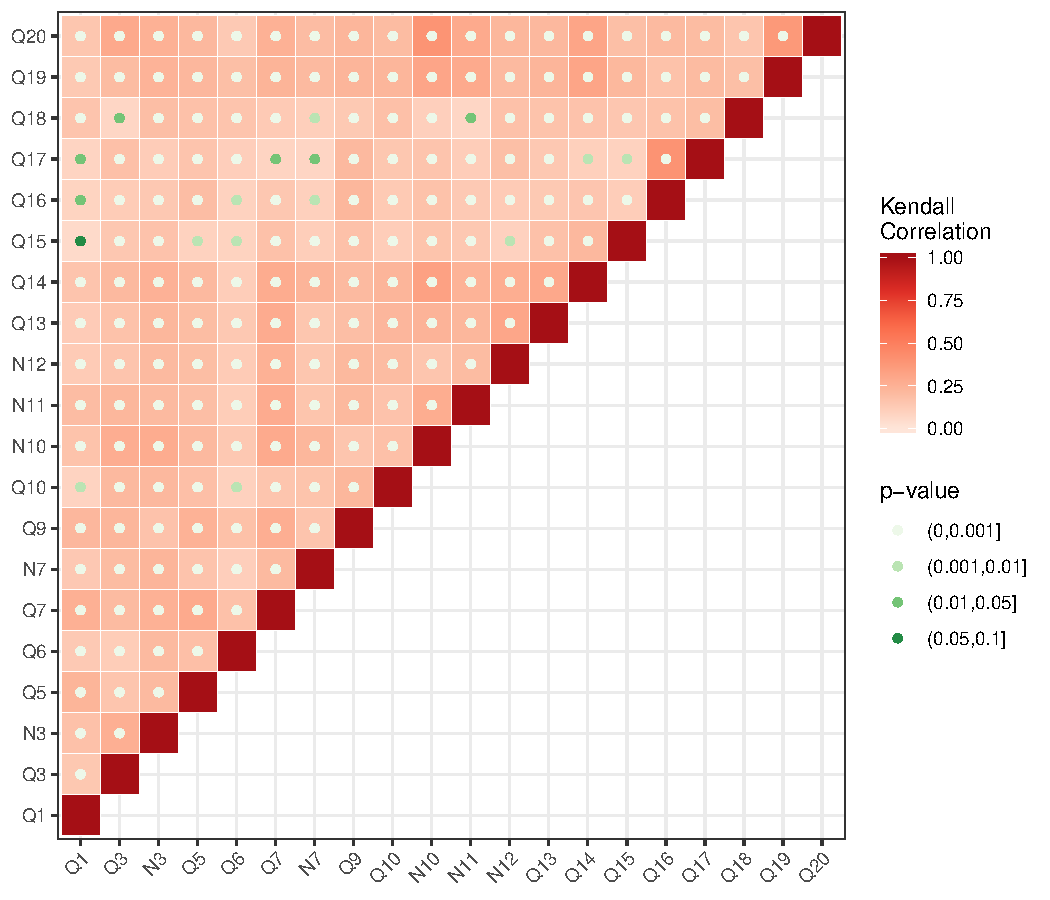
\includegraphics[width=\linewidth]{fig/IMPRV_cor_17.pdf}
  \caption{\label{fig:IMPRV_cor_17}Correlation heat map and significance indicators of Kendall's $\tau$ test}
\end{figure}

The six largest p-values of the Kendall's $\tau$ test are shown in Table~\ref{tab:IMPRV_cortest}. The p-value of the test of the correlation between Q1 and Q15 is 0.0907, indicating the null hypothesis cannot be rejected at 95\% significance level. However, the significance probability of the same test using the data from previous MDTs is $4.14 \times 10^{-7}$ and the Kendall correlation between Q1 and Q15 is 0.08 (Figure~\ref{fig:IRT_cor_pre17}), suggesting the correlation exists. According to the mathematics taxonomy provided by the report last year, both Q1 and Q15 are Type-A questions and require routine use of procedures \cite{lastyear}. %Given that relatively small sample size of the data from MDT2017, which contains 896 students, the result may driven by 

\begin{table}[ht]
  \centering
  \begin{tabular}{ccc}
    \hline
  Item $i$ & Item $j$ & pvals \\ 
    \hline
  Q1 & Q15 & 0.0907 \\ 
    Q3 & Q18 & 0.0351 \\ 
    N11 & Q18 & 0.0273 \\ 
    N7 & Q17 & 0.0265 \\ 
    Q1 & Q17 & 0.0160 \\ 
    Q7 & Q17 & 0.0141 \\ 
     \hline
  \end{tabular}
  \caption{\label{tab:IMPRV_cortest}Six largest p-values of Kendall's $\tau$ test}
\end{table}

\subsection{Dimensionality}

A scree plot of the eigenvalues for a principal axis factor analysis and the plots of simulated and resampled data are shown in Figure~\ref{fig:IMPRV_EFA_scree}. The eigenvalue of factor number 2 decreases significantly and the difference between simulated data and actual data is minimised at the point of factor number 7, suggesting that an integer between 1 and 7 would be a good choice for the number of factors to be extracted. This result is similar to the interpretation of the scree plots in Figure~\ref{fig:EFA_scree}. 

\begin{figure}[H]
  \centering
  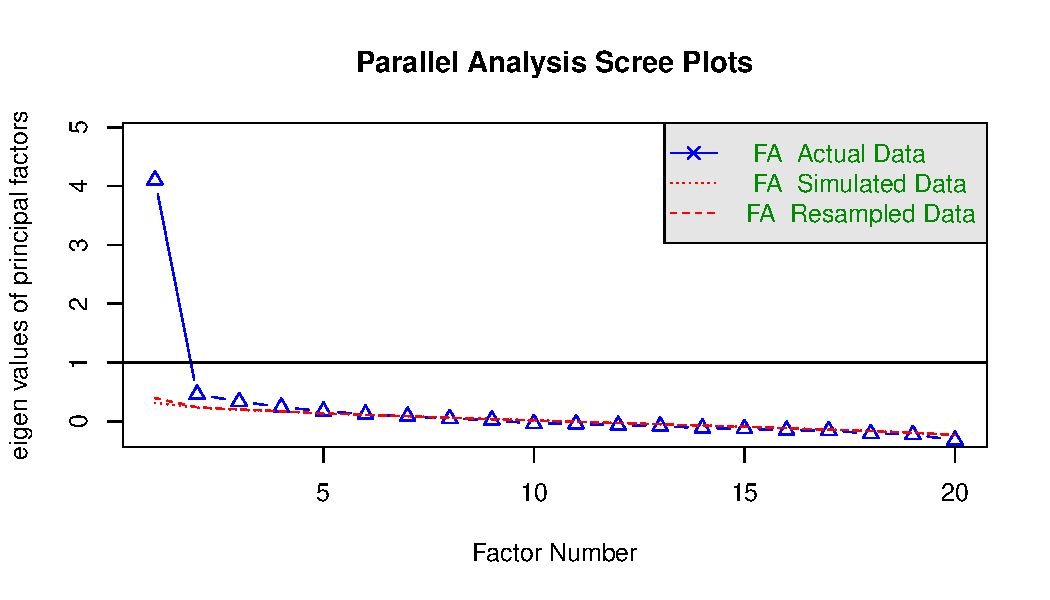
\includegraphics[width=\linewidth]{fig/IMPRV_EFA_scree.pdf}
  \caption{\label{fig:IMPRV_EFA_scree}Parallel analysis scree plots}
\end{figure}

In Table~\ref{tab:IMPRV_EFA_17_1} are shown the standardised loadings of items on the factor of a one-factor exploratory factor analysis (EFA) model. All the loadings of the items are significant, with 0.321 being the smallest factor loading. 

\begin{table}[ht]
  \begin{minipage}{0.5\linewidth}
    \centering
    \begin{tabular}{lccc}
      \hline
     & Type & MR1 & \\ 
      \hline
    Q1 & A & 0.322 & * \\ 
      Q3 & B & 0.437 & * \\ 
      N3 & A & 0.524 & * \\ 
      Q5 & A & 0.441 & * \\ 
      Q6 & A & 0.308 & * \\ 
      Q7 & B & 0.521 & * \\ 
      N7 & B & 0.375 & * \\ 
      Q9 & A & 0.459 & * \\ 
      Q10 & B & 0.436 & * \\ 
      N10 & B & 0.598 & * \\ 
       \hline
    \end{tabular}
  \end{minipage}%
  \begin{minipage}{0.5\linewidth}
    \centering
    \begin{tabular}{lccc}
      \hline
     & Type & MR1 & \\ 
      \hline
    N11 & C & 0.486 & * \\ 
      N12 & A & 0.467 & * \\ 
      Q13 & A & 0.495 & * \\ 
      Q14 & B & 0.575 & * \\ 
      Q15 & A & 0.328 & * \\ 
      Q16 & A & 0.352 & * \\ 
      Q17 & A & 0.338 & * \\ 
      Q18 & A & 0.321 & * \\ 
      Q19 & B & 0.536 & * \\ 
      Q20 & B & 0.556 & * \\ 
       \hline
    \end{tabular}
  \end{minipage}
  \caption{\label{tab:IMPRV_EFA_17_1}Loadings of items on factor where `*' indicates loadings greater or equal to 0.25}
\end{table}

The loadings are also plotted along the Factor 1 axis in Figure~\ref{fig:IMPRV_EFA_17_2}. Comparing with Figure~\ref{fig:EFA_pre17_2}, all questions in MDT3 have loadings on the factor higher than 0.3, while two of the questions in MDT2 do not. N7, one of the new Type-B questions in MDT3, has relatively lower loadings than other Type-B questions. The new Type-C question, N11, has higher loading than most of the Type-A questions, but it is not comparable with Type-B questions because there is only one Type-C question in the test and has mid-level of loading. 

\begin{figure}[H]
  \centering
  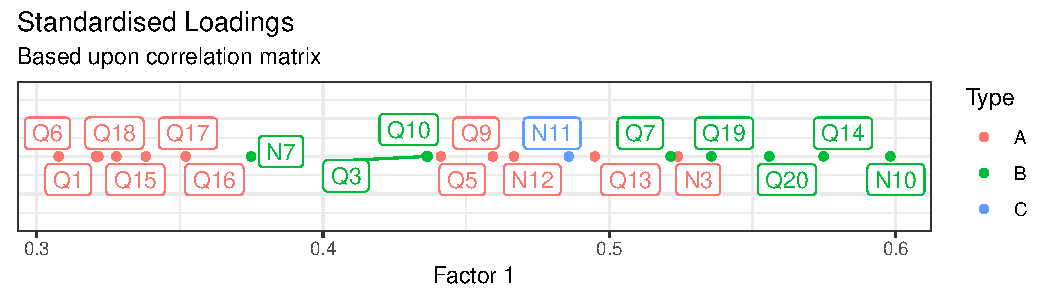
\includegraphics[width=\linewidth]{fig/IMPRV_EFA_17_1.pdf}
  \caption{\label{fig:IMPRV_EFA_17_1}Standardised loadings on Factor 1}
\end{figure}

An additional factor is added to the EFA model in the next step to examine whether the results are improved. The loadings of the items on the two factors which are greater or equal to 0.25 are shown in Table~\ref{tab:IMPRV_EFA_17_2}. In this model, the item Q18 becomes non-significant, which has approximately 0.2 loadings on both factors before they are cut off. Q16 and Q17 have significant loadings only on Factor 2 in contrast to other items, which is the same case as in Table~\ref{tab:EFA_pre17_2}. 

\begin{table}[ht]
  \begin{minipage}{0.5\linewidth}
    \centering
    \begin{tabular}{lccc}
      \hline
     & Type & MR1 & MR2 \\ 
      \hline
    Q1 & A & 0.329 &  \\ 
      Q3 & B & 0.418 &  \\ 
      N3 & A & 0.500 &  \\ 
      Q5 & A & 0.382 &  \\ 
      Q6 & A & 0.275 &  \\ 
      Q7 & B & 0.575 &  \\ 
      N7 & B & 0.407 &  \\ 
      Q9 & A & 0.355 &  \\ 
      Q10 & B & 0.370 &  \\ 
      N10 & B & 0.643 &  \\ 
       \hline
    \end{tabular}
  \end{minipage}%
  \begin{minipage}{0.5\linewidth}
    \centering
    \begin{tabular}{lccc}
      \hline
     & Type & MR1 & MR2 \\ 
      \hline
    N11 & C & 0.507 &  \\ 
      N12 & A & 0.405 &  \\ 
      Q13 & A & 0.479 &  \\ 
      Q14 & B & 0.624 &  \\ 
      Q15 & A & 0.311 &  \\ 
      Q16 & A &  & 0.511 \\ 
      Q17 & A &  & 0.704 \\ 
      Q18 & A &  &  \\ 
      Q19 & B & 0.503 &  \\ 
      Q20 & B & 0.532 &  \\ 
       \hline
    \end{tabular}
  \end{minipage}
  \caption{\label{tab:IMPRV_EFA_17_2}Loadings of items on factors which are greater or equal to 0.25 only}
\end{table}

In Figure~\ref{fig:IMPRV_EFA_17_2} is shown the scatter plot of the standardised loadings on both factors. The items loaded heavily on Factor 1 are more divergent from the items loaded heavily on Factor 2, comparing with the loadings of the questions from previous MDTs showing in Figure~\ref{fig:EFA_pre17_2}. 

\begin{figure}[H]
  \centering
  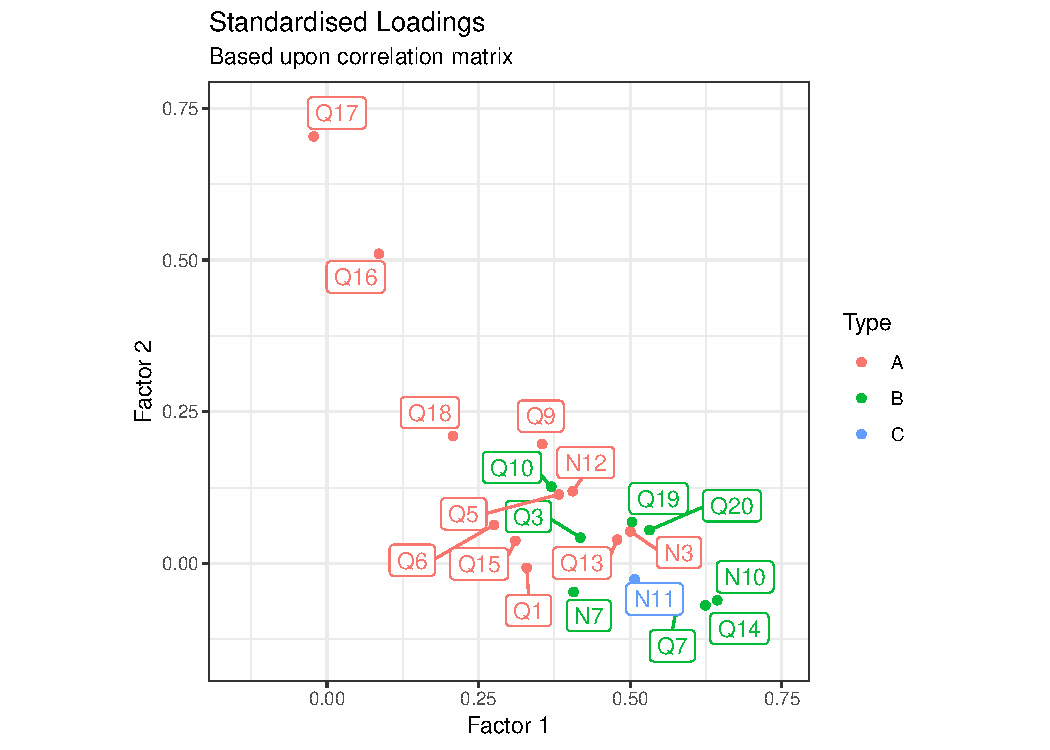
\includegraphics[width=\linewidth]{fig/IMPRV_EFA_17_2.pdf}
  \caption{\label{fig:IMPRV_EFA_17_2}Standardised loadings on Factor 2 against Factor 1}
\end{figure}

The statistics representing the adequacy of the model, including RMSR, RMSEA and Tucker Lewis Index seem to be satisfactory in both one-factor and two-factor EFA models. When the number of factors in the EFA models was increased to 3, 4 or more, the simple-structure (i.e. all items have significant but single loading) of the items does not hold. Therefore, either one-factor or two-factor model should be chosen for further analyses of the data of MDT3. 

In Chapter~\ref{chap:PCM_pre17}, the one-factor structure of the latent ability is chosen because of the simplicity of interpretation. Since the multidimensional PCM functions of \texttt{ltm} and \texttt{mirt} packages cannot work with non-standard scoring functions (e.g. questions scored 0, 2, 3, 5), it would be difficult to proceed with a multi-factor model. Additionally, our aim is to compare MDT2 and MDT3 and we will continue with the one-factor structure. 

However, it is worthwhile and necessary to analyse the two-dimensional model for all data, with self-defined functions for computing inferences with modified scoring functions in the future. 

\section{Separate calibration}

Under the equating method of separate calibration with linear transformation, a generalised partial credit model (Model \texttt{MDT3-GPCM}) is fitted to to the data from MDT3 separately. 

The item response curves, test response curve, item information curves and test information curve based on the untransformed parameters are shown in Figure~\ref{fig:IMPRV_17}. It can be seen that the new question N10 has the highest information at the range of positive ability. 

\begin{figure}[H]
  \centering
  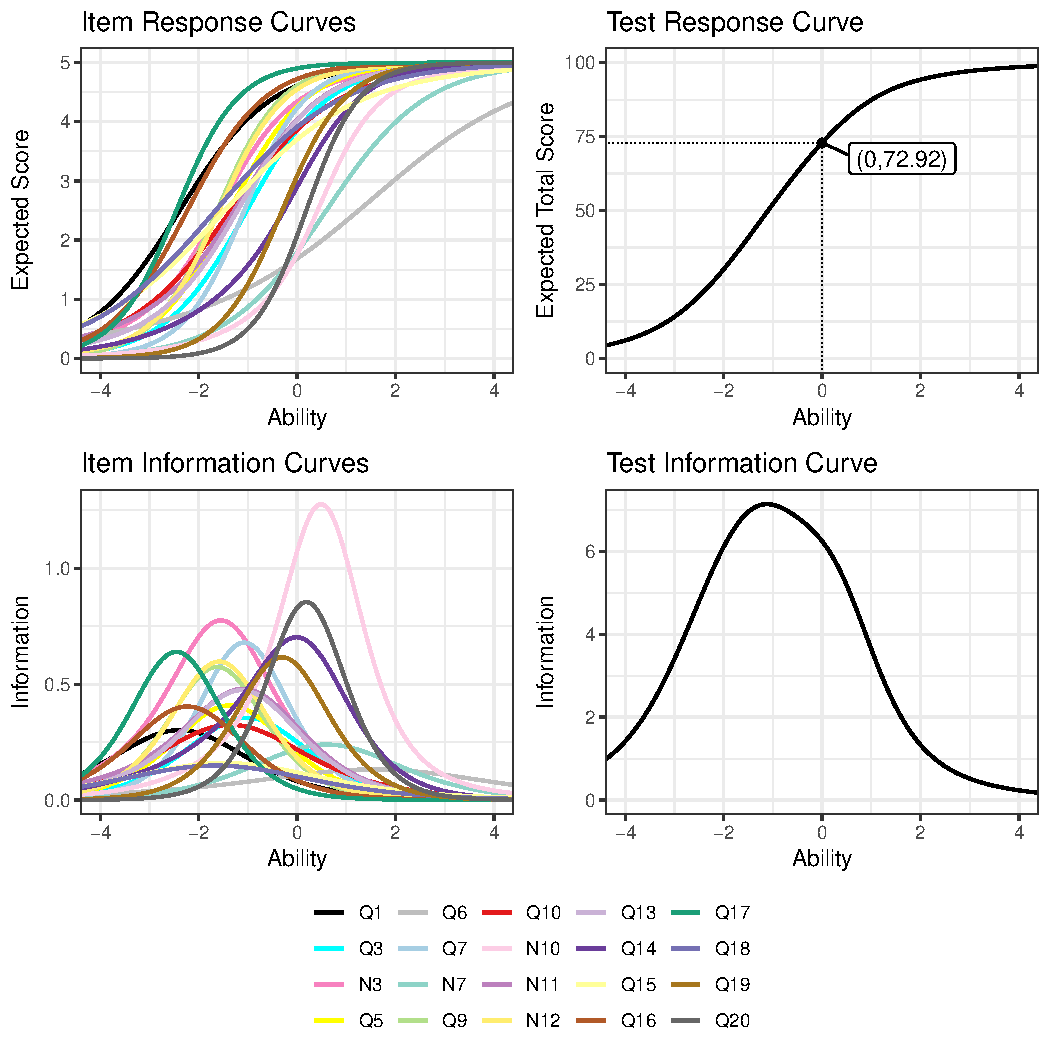
\includegraphics[width=\linewidth]{fig/IMPRV_17.pdf}
  \caption{\label{fig:IMPRV_17}Plots of GPCM using separate calibration (Model \texttt{MDT3-GPCM})}
\end{figure}

To place all the students on the comparable scale of ability and examine how the accuracy of estimating ability changes, the linear relationship between the difficulty parameters $d_{ik}$ of the equating items is determined. 

The scatter plot and of the difficulty parameters and the linear regression line with confidence intervals are shown in Figure~\ref{fig:IMPRV_SC_lm}. The regression of the difficulty parameters of Model \texttt{MDT3-GPCM} $d^*$ on those of Model \texttt{MDT2-GPCM} $d$ is estimated by 

$$d^* = 0.05 + 0.94 d \text{. }$$

\begin{figure}[H]
  \centering
  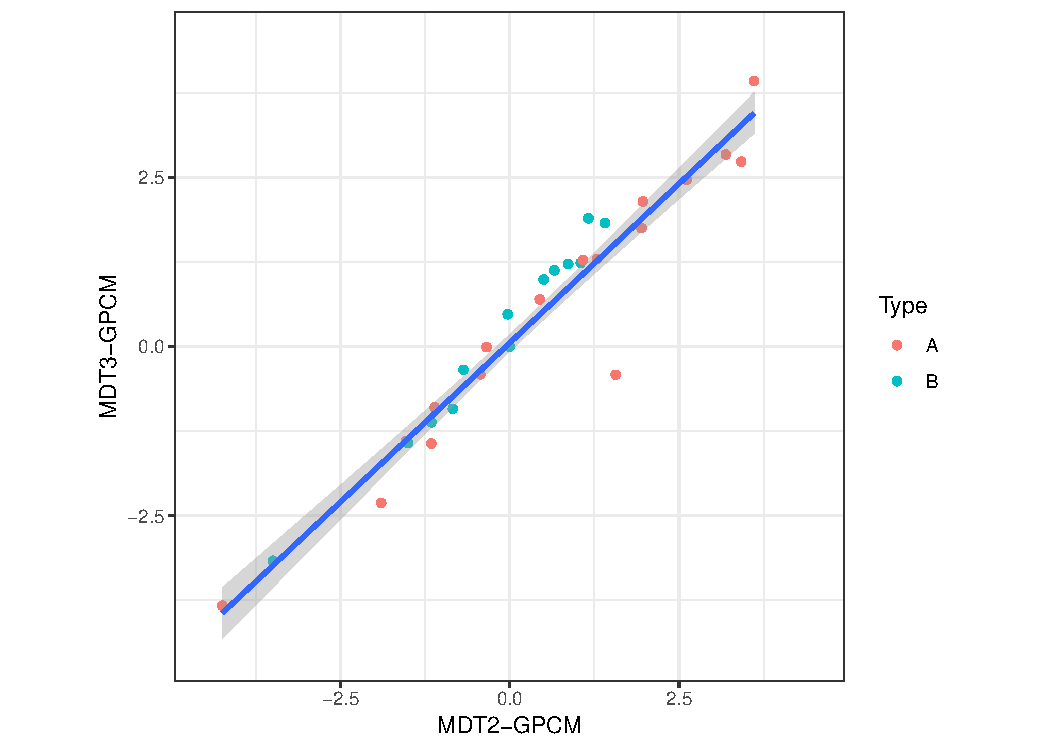
\includegraphics[width=\linewidth]{fig/IMPRV_SC_lm.pdf}
  \caption{\label{fig:IMPRV_SC_lm}Difficulty parameters of Model \texttt{MDT2-GPCM} and Model \texttt{MDT3-GPCM} and the linear regression line}
\end{figure}

This linear transformation is applied to the difficulty parameters of all the items from Model \texttt{MDT3-GPCM}. The item response curves, test response curve, item information curves and test information curve with linear transformation of the new model (Model \texttt{MDT3-SC}) are plotted in Figure~\ref{fig:IMPRV_17_SC}. These plots are now comparable with the plots of Model \texttt{MDT2-GPCM} (Figure~\ref{fig:IRT_pre17_GPCM}), because of the common metric between both calibrations. 

\begin{figure}[H]
  \centering
  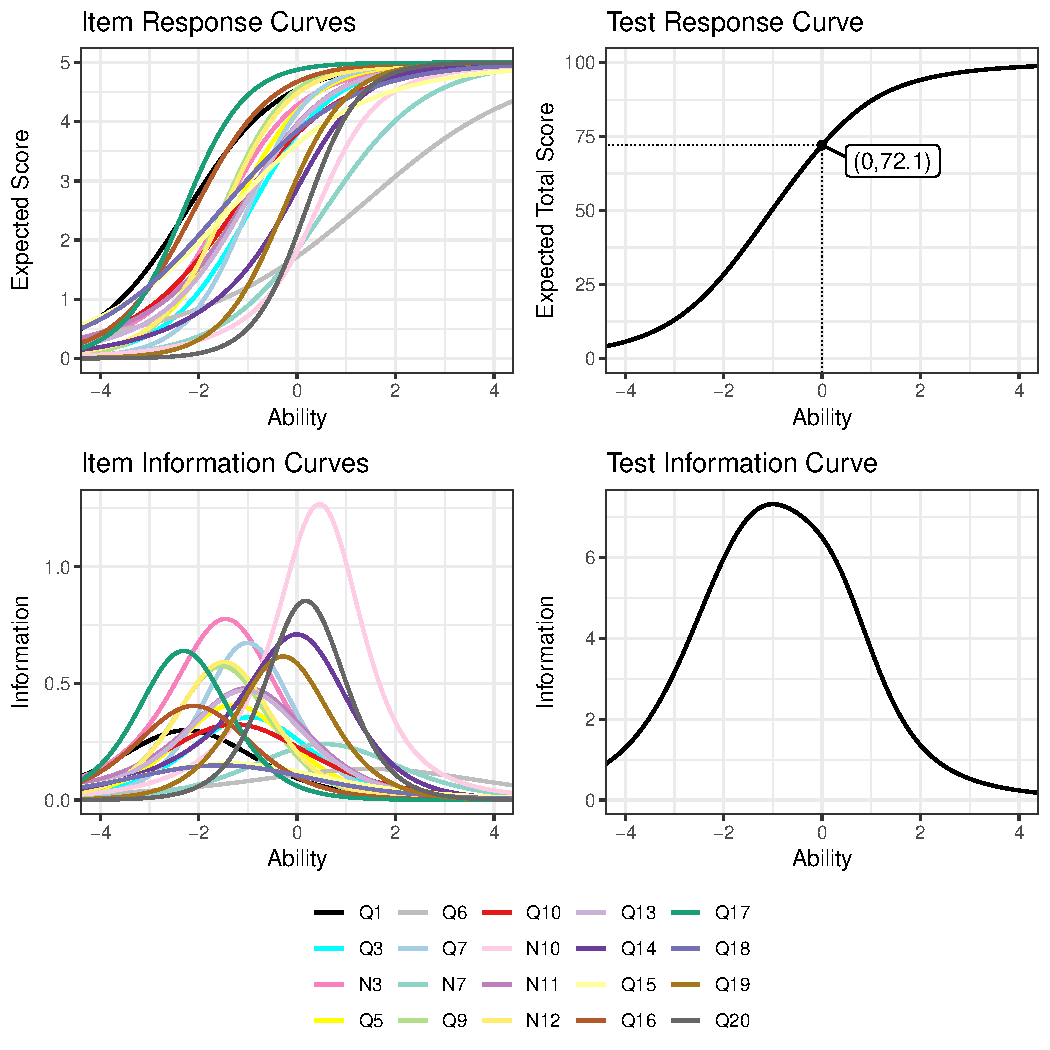
\includegraphics[width=\linewidth]{fig/IMPRV_17_SC.pdf}
  \caption{\label{fig:IMPRV_17_SC}Plots of GPCM using separate calibration with linear transformation (Model \texttt{MDT3-SC})}
\end{figure}

The expected total score of a student with ability 0 after transforming the parameters is 72.1, while the expected total score is 72.92 before transforming, indicating the students from 2017 have higher ability than the students admitted before 2017. However, due to the limited functions in the package \texttt{mirt}, the estimated abilities of students are not yet available to be computed. 

\section{FCIP calibration}

Under the equating method of fixed common item parameter calibration, the parameters of the equating items in the GPCM on the new test (Model \texttt{MDT3-FCIP}) are fixed to the estimated values of parameters in the GPCM on the old test (Model \texttt{MDT2-GPCM}). The item and test response curves and information curves are shown in Figure~\ref{fig:IMPRV_17_FCIP}. In this calibration, the scale of the ability axis, the response and information curves of the equating items, are exactly the same as Model \texttt{MDT2-GPCM}. 

\begin{figure}[H]
  \centering
  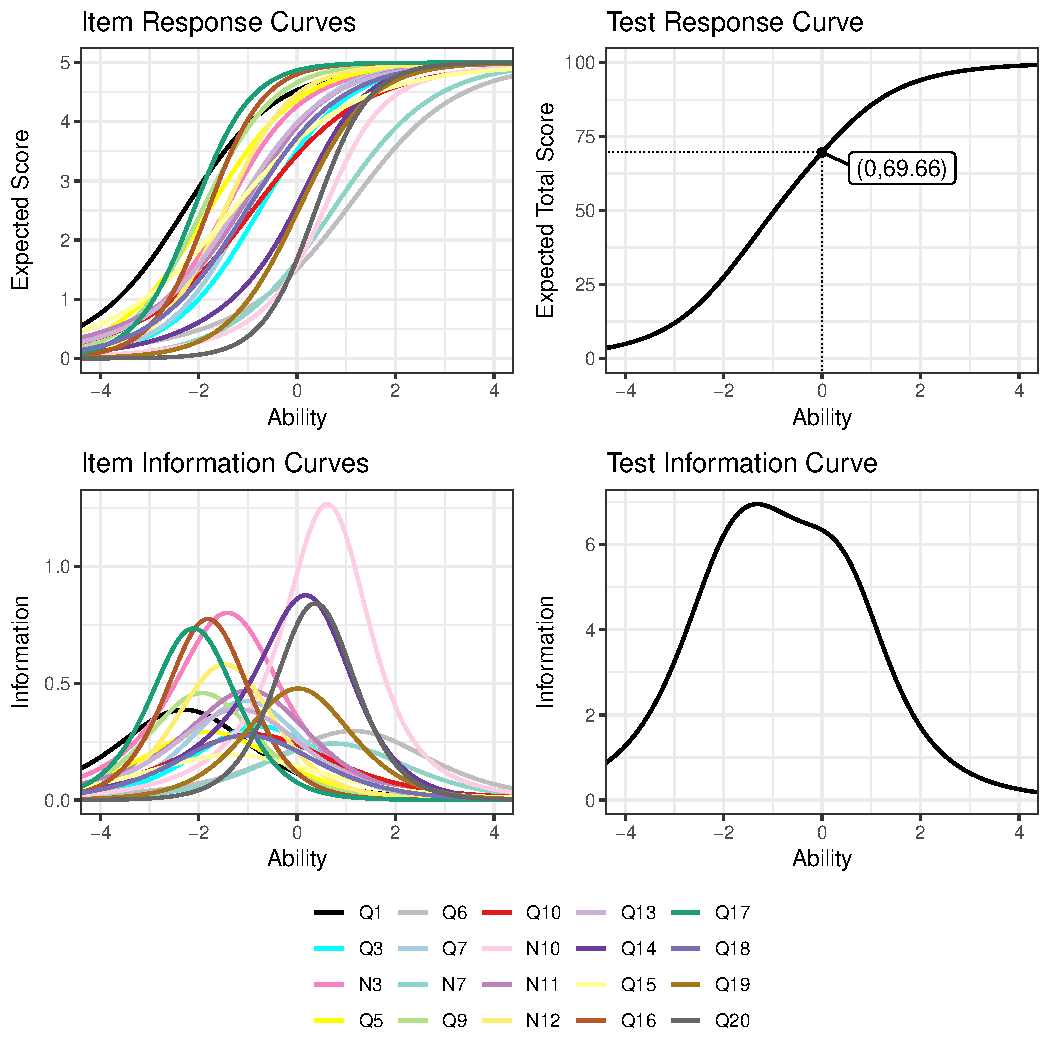
\includegraphics[width=\linewidth]{fig/IMPRV_17_FCIP.pdf}
  \caption{\label{fig:IMPRV_17_FCIP}Plots of GPCM using fixed common item parameter calibration (Model \texttt{MDT3-FCIP})}
\end{figure}

The increase of accuracy of estimating the abilities of students is one of the indices that determine the improvement of MDT. According to the definition of item information and standard error of measurement (SEM), a higher item information will lower the SEM and narrow the confidence intervals of the estimated abilities. 

The item response curves shown in Figure~\ref{fig:IMPRV_FCIP_cf} and the expected scores of the students with average ability and the changes of the expectations of the students with ability $\pm 2$ shown in Table~\ref{tab:IMPRV_FCIP_expscore} can be used for comparing the changes in discriminations and difficulties of the new questions and the removed questions.

N3 and N12, which are the same questions as Q4 and Q12 but with different marking schemes, are more discriminating but an average student can score higher marks under the new marking schemes. Additionally, the abilities of a student who score half of the marks are estimated at approximately the same values under both marking schemes. The rest of the new questions, N7, N10 and N11, are much more discriminating and difficult than the questions suggested to be removed. 

\begin{figure}[H]
  \centering
  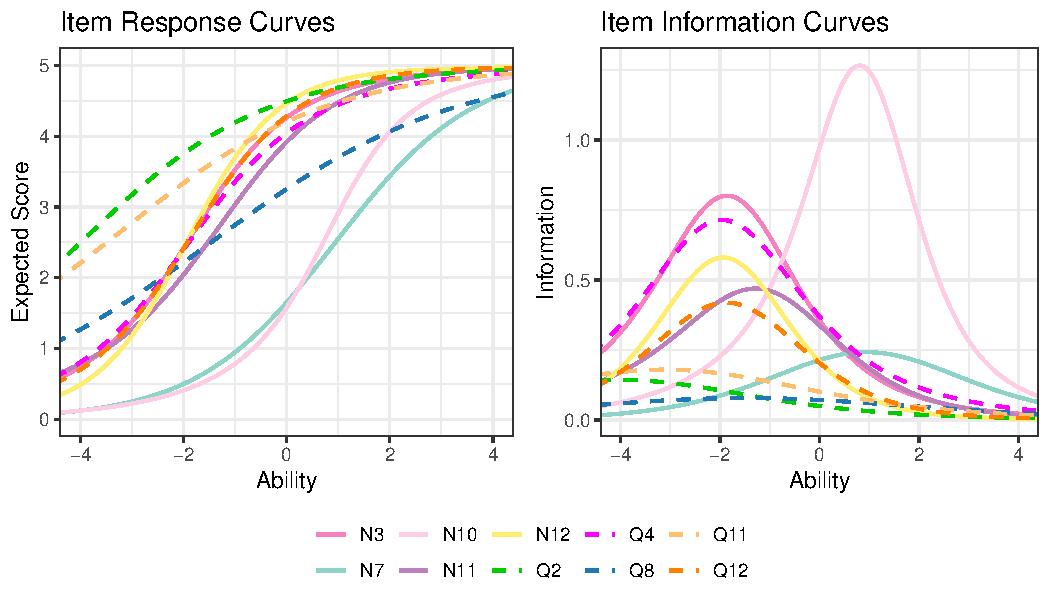
\includegraphics[width=\linewidth]{fig/IMPRV_FCIP_cf.pdf}
  \caption{\label{fig:IMPRV_FCIP_cf}Item response curves and item information curves of added items in MDT3 of Model \texttt{MDT3-FCIP} and removed items from the previous test of Model \texttt{MDT2-GPCM}}
\end{figure}

\begin{table}[ht]
  \centering
  \begin{tabular}{ccccc}
    \hline
   & $\bar T_i (-2) - \bar T_i (0)$ & Facility & $\bar T_i (2) - \bar T_i (0)$ & Discrimination \\ 
   \hline
   N3 (Q4) & -2.54 & 4.26 & 0.61 & 3.15 \\ 
     N12 (Q12) & -2.88 & 4.47 & 0.47 & 3.35 \\ 
     N7 & -1.33 & 1.65 & 2.24 & 3.57 \\ 
     N10 & -1.30 & 1.58 & 2.87 & 4.17 \\ 
     N11 & -2.40 & 3.92 & 0.93 & 3.34 \\ 
     \hline
     Sum.add & -10.46 & 15.88 & 7.13 & 17.58 \\ 
     \hline
     Q4 & -2.27 & 4.05 & 0.71 & 2.99 \\ 
     Q12 & -2.57 & 4.29 & 0.62 & 3.19 \\ 
     Q2 & -1.09 & 4.49 & 0.36 & 1.46 \\ 
     Q8 & -1.36 & 3.25 & 1.00 & 2.36 \\ 
     Q11 & -1.22 & 4.21 & 0.54 & 1.76 \\ 
     \hline
     Sum.rm & -8.51 & 20.29 & 3.24 & 11.76 \\ 
     \hline
  \end{tabular}
  \caption{\label{tab:IMPRV_FCIP_expscore}Expected scores of students with ability -2, 0 and 2}
\end{table}

The item information curves shown in Figure~\ref{fig:IMPRV_FCIP_cf} and the major and total item information areas for the new and removed questions shown in Table~\ref{tab:IMPRV_FCIP_summaryiif} can be used for comparing the changes in information of the new and removed questions. 

The item information functions of N3 and N12 attain their maximum at approximately the same values of ability as Q4 and Q12 respectively. Their information areas over the whole range of ability increase slightly, as well as the areas over the range -2 to 2. However, the information areas for the above-average students drop slightly in these two questions. The new questions have much larger information areas than the questions suggested to be removed, especially N10. 

\begin{table}[ht]
  \centering
  \begin{tabular}{rr|rrr|rrr}
    \hline
    & & \multicolumn{3}{c|}{Major Info Area} & \multicolumn{3}{c}{Total Info Area} \\
   & Max at & Lower & Upper & Total & Lower & Upper & Total \\ 
   \hline
   N3 & -1.41 & 1.32 & 0.31 & 1.63 & 2.21 & 0.38 & 2.59 \\ 
     N12 & -1.47 & 0.91 & 0.15 & 1.06 & 1.41 & 0.17 & 1.58 \\ 
     N7 & 0.72 & 0.26 & 0.44 & 0.70 & 0.32 & 0.66 & 0.98 \\ 
     N10 & 0.61 & 0.87 & 1.92 & 2.80 & 1.06 & 2.29 & 3.35 \\ 
     N11 & -0.98 & 0.84 & 0.33 & 1.17 & 1.37 & 0.38 & 1.75 \\ 
     \hline
     Q4 & -1.49 & 1.21 & 0.38 & 1.59 & 2.15 & 0.51 & 2.66 \\ 
     Q12 & -1.42 & 0.71 & 0.17 & 0.88 & 1.18 & 0.20 & 1.37 \\ 
     Q2 & -3.04 & 0.17 & 0.06 & 0.23 & 0.70 & 0.08 & 0.78 \\ 
     Q8 & -1.11 & 0.15 & 0.11 & 0.26 & 0.36 & 0.20 & 0.56 \\ 
     Q11 & -2.36 & 0.29 & 0.13 & 0.42 & 1.00 & 0.19 & 1.19 \\ 
      \hline
  \end{tabular}
  \caption{\label{tab:IMPRV_FCIP_summaryiif}The area under each item information curve over different definite integral ranges}
\end{table}

In Figure~\ref{fig:IMPRV_FCIP_tifcf} are shown the sums of item information functions of the two different question sets, where the improvement of estimating ability can be seen clearly. 

\begin{figure}[H]
  \centering
  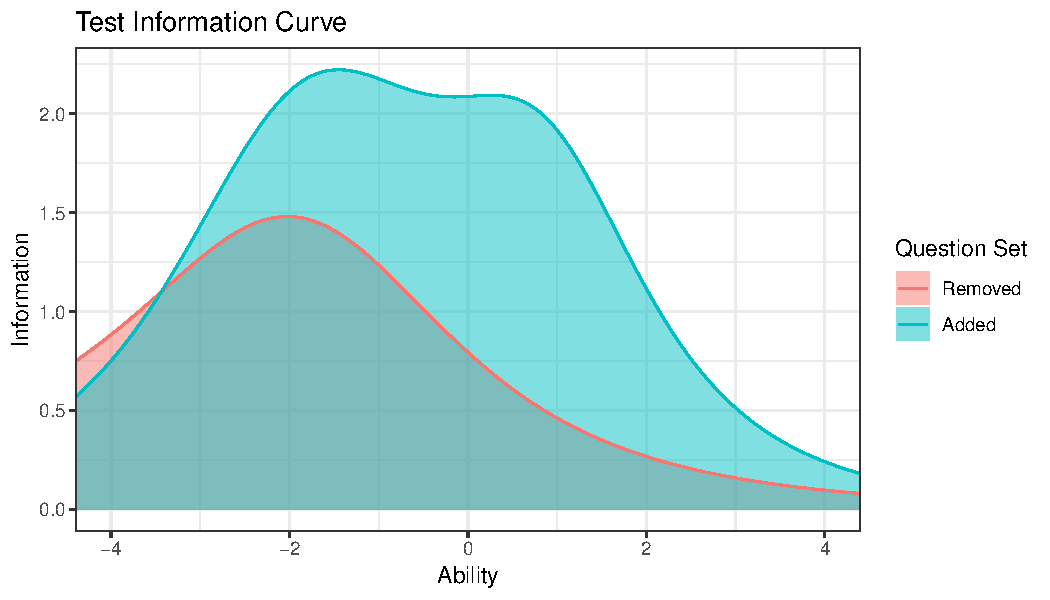
\includegraphics[width=\linewidth]{fig/IMPRV_FCIP_tifcf.pdf}
  \caption{\label{fig:IMPRV_FCIP_tifcf}Sums of item information functions of different sets of questions}
\end{figure}

The test information function attains its maximum at $\theta=-1.32$, which is shown in Table~\ref{tab:IMPRV_FCIP_summarytif}. Comparing with the test information of Model \texttt{MDT2-GPCM} in Table~\ref{tab:IRT_pre17_summaryiif}, the area over the range of positive ability increases significantly. 

\begin{table}[ht]
  \centering
  \begin{tabular}{rr|rrr|rrr}
    \hline
    & & \multicolumn{3}{c|}{Major Info Area} & \multicolumn{3}{c}{Total Info Area} \\
   & Max at & Lower & Upper & Total & Lower & Upper & Total \\ 
   \hline
   Test Information & -1.32 & 13.38 & 8.50 & 21.87 & 21.76 & 10.31 & 32.07 \\ 
      \hline
  \end{tabular}
  \caption{\label{tab:IMPRV_FCIP_summarytif}The area under the test information curve of Model \texttt{MDT3-FCIP} over different definite integral ranges}
\end{table}

In Table~\ref{tab:IMPRV_FCIP_info} are shown the major and total item information areas and their proportions of the test information in Model \texttt{MDT2-GPCM}. In terms of major information area, the test information area increases by 22.29\% in MDT3. The new questions N10 and N11 account for a large proportion of the increase, while N7 is the least informative among the new questions. 

\begin{table}[ht]
  \begin{minipage}{0.5\linewidth}
      \centering
      \begin{tabular}{lcrr}
        \hline
      Item & Type & MajorInfo & Prop (\%) \\ 
      \hline
      Q15 & A & 0.54 & 3.02 \\ 
        Q5 & A & 0.58 & 3.25 \\ 
        Q1 & A & 0.60 & 3.37 \\ 
        Q9 & A & 0.70 & 3.92 \\ 
        N7 & B & 0.70 & 3.93 \\ 
        Q18 & A & 0.73 & 4.09 \\ 
        Q17 & A & 0.78 & 4.35 \\ 
        Q10 & B & 0.82 & 4.58 \\ 
        Q6 & A & 0.83 & 4.62 \\ 
        Q3 & B & 0.85 & 4.75 \\ 
        Q13 & A & 0.95 & 5.29 \\ 
        Q7 & B & 1.00 & 5.62 \\ 
        Q16 & A & 1.02 & 5.71 \\ 
        N12 & A & 1.06 & 5.94 \\ 
        N11 & C & 1.17 & 6.54 \\ 
        Q19 & B & 1.22 & 6.81 \\ 
        N3 & A & 1.63 & 9.11 \\ 
        Q20 & B & 1.72 & 9.64 \\ 
        Q14 & B & 2.17 & 12.11 \\ 
        N10 & B & 2.80 & 15.64 \\ 
        \hline
        Sum & & 21.87 & 122.29 \\
         \hline
      \end{tabular}
  \end{minipage}%
  \begin{minipage}{0.5\linewidth}
    \centering
    \begin{tabular}{lcrr}
      \hline
    Item & Type & TotalInfo & Prop (\%) \\ 
    \hline
    Q15 & A & 0.98 & 3.46 \\ 
      N7 & B & 0.98 & 3.47 \\ 
      Q18 & A & 1.05 & 3.71 \\ 
      Q5 & A & 1.08 & 3.81 \\ 
      Q3 & B & 1.12 & 3.96 \\ 
      Q10 & B & 1.28 & 4.52 \\ 
      Q6 & A & 1.34 & 4.71 \\ 
      Q7 & B & 1.35 & 4.77 \\ 
      Q9 & A & 1.35 & 4.77 \\ 
      Q19 & B & 1.38 & 4.87 \\ 
      Q13 & A & 1.46 & 5.13 \\ 
      Q1 & A & 1.49 & 5.25 \\ 
      N12 & A & 1.58 & 5.58 \\ 
      Q17 & A & 1.71 & 6.04 \\ 
      N11 & C & 1.75 & 6.18 \\ 
      Q16 & A & 1.76 & 6.20 \\ 
      Q20 & B & 1.84 & 6.47 \\ 
      N3 & A & 2.59 & 9.13 \\ 
      Q14 & B & 2.61 & 9.20 \\ 
      N10 & B & 3.35 & 11.82 \\ 
      \hline
      Sum & & 32.07 & 113.04 \\
       \hline
    \end{tabular}
  \end{minipage}
  \caption{\label{tab:IMPRV_FCIP_info}Tables of item information of Model \texttt{MDT3-FCIP} and corresponding proportions of test information in Model \texttt{MDT2-GPCM}}
\end{table}

The density plots of the estimated abilities of the students taking two different tests using the method of EAP are shown in Figure~\ref{fig:IMPRV_FCIP_eap}, where there is a trend that the distribution of the students examined in 2017 shifts to the right. 

\begin{figure}[H]
  \centering
  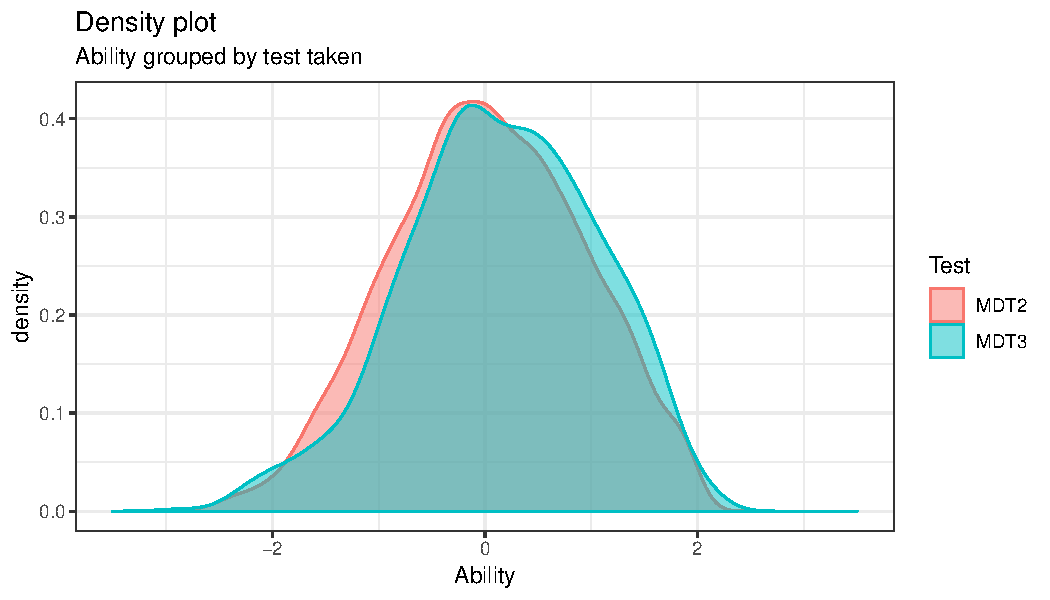
\includegraphics[width=\linewidth]{fig/IMPRV_FCIP_eap.pdf}
  \caption{\label{fig:IMPRV_FCIP_eap}Density plots of the estimated abilities of students grouped by the test taken}
\end{figure}

The mean of the estimated abilities of the students taking MDT3 shown in Table~\ref{tab:IMPRV_FCIP_eap_dsc} are higher than the students taking MDT2. The K-S test of these two sets of estimated abilities suggests that the students are drawn from different distributions of ability (with p-value 0.002). 

\begin{table}[ht]
  \centering
  \begin{tabular}{rrrrrrrr}
    \hline
   & n & mean & sd & min & max & skew & kurtosis \\ 
    \hline
  MDT2 & 3248 & 0.02 & 0.90 & -2.73 & 1.86 & -0.09 & -0.48 \\ 
    MDT3 & 896 & 0.15 & 0.90 & -2.87 & 2.04 & -0.26 & -0.26 \\ 
     \hline
  \end{tabular}
  \caption{\label{tab:IMPRV_FCIP_eap_dsc}Basic descriptive statistics of the distributions of the estimated abilities}
\end{table}

\section{Concurrent parameter calibration}

Under the equating method of concurrent parameter calibration, a generalised partial credit model (Model \texttt{MDT3-CP}) is fitted to the data of all the students taking MDT2 and MDT3 together. 

The item and test response curves and information curves are plotted in Figure~\ref{fig:IMPRV_17_CP}. The red curves in the test response curve and information curve plots represent the questions from MDT2, while the turquoise curves represent the questions in MDT3. It can be seen that the test response curve of MDT3 is on the right of the curve of MDT2, indicating that the MDT3 is more difficult. The test information curve of the MDT3 is higher than the old test, which is consistent with the findings from Model \texttt{MDT3-FCIP}. 

\begin{figure}[H]
  \centering
  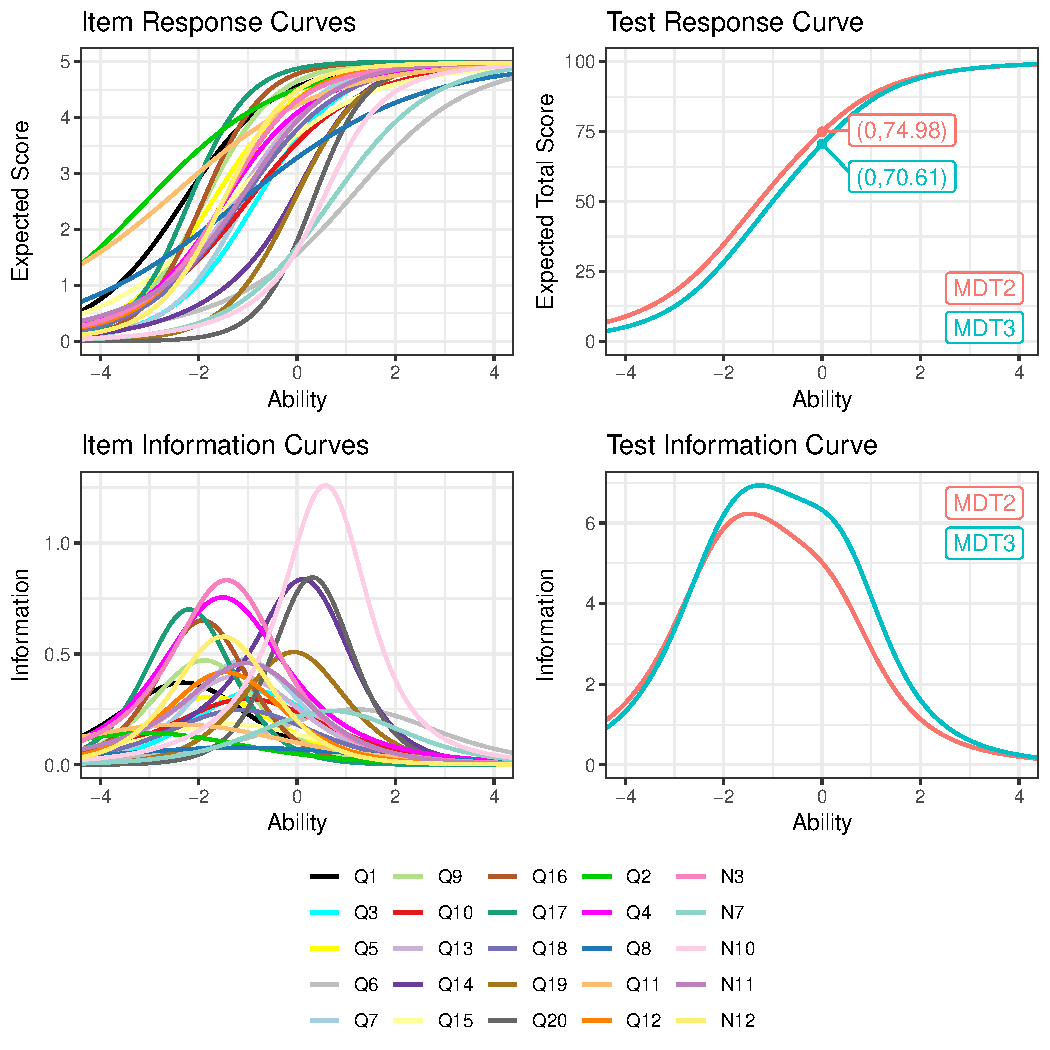
\includegraphics[width=\linewidth]{fig/IMPRV_17_CP.pdf}
  \caption{\label{fig:IMPRV_17_CP}Plots of GPCM using concurrent parameter calibration (Model \texttt{MDT3-CP})}
\end{figure}

The item response curves and the item information curves for the new questions and the removed questions are shown separately in Figure~\ref{fig:IMPRV_CP_cf}. It should be noted that the plots are similar to the plots of Model \texttt{MDT3-FCIP} in Figure~\ref{fig:IMPRV_FCIP_cf}. 

\begin{figure}[H]
  \centering
  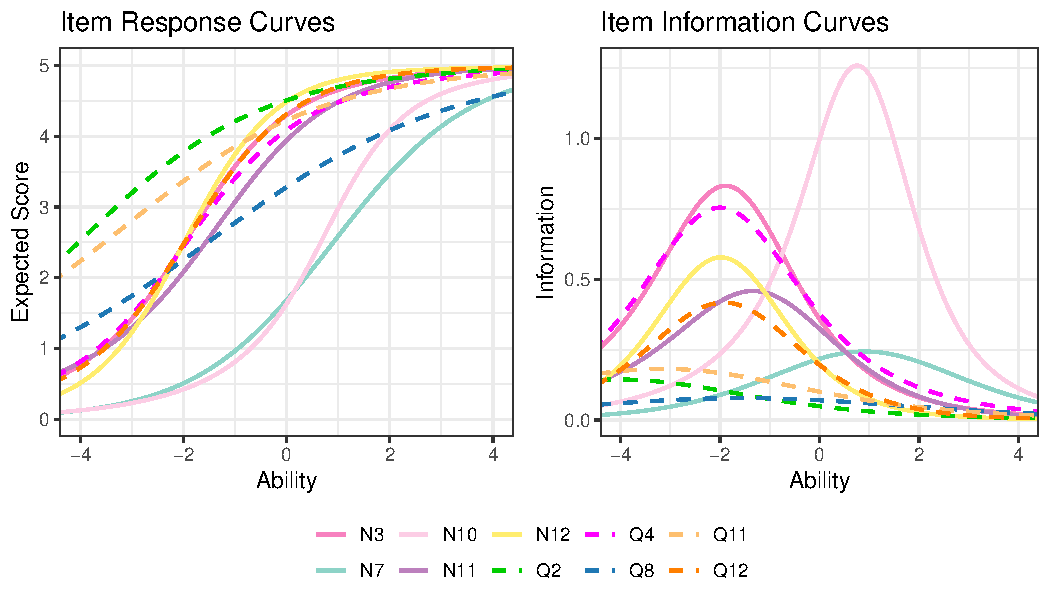
\includegraphics[width=\linewidth]{fig/IMPRV_CP_cf.pdf}
  \caption{\label{fig:IMPRV_CP_cf}Item response curves and item information curves of added items in MDT3 and removed items from the previous test of Model \texttt{MDT3-CP}}
\end{figure}

The major and total information areas and their proportions of the sum of information areas of the 25 questions are shown in Table~\ref{tab:IMPRV_CP_info}, where items in italic style are the questions removed from the test and items in bold style are the new questions. 

\begin{table}[ht]
  \begin{minipage}{0.5\linewidth}
      \centering
      \begin{tabular}{>{\rowmac}l>{\rowmac}c>{\rowmac}r>{\rowmac}r<{\clearrow}}
        \hline
      Item & Type & MajorInfo & Prop (\%) \\ 
      \hline
    \setrow{\itshape}Q2 & A & 0.23 & 0.90 \\ 
    \setrow{\itshape}Q8 & A & 0.26 & 1.04 \\ 
    \setrow{\itshape}Q11 & A & 0.41 & 1.66 \\ 
      Q15 & A & 0.51 & 2.06 \\ 
      Q1 & A & 0.56 & 2.25 \\ 
      Q5 & A & 0.62 & 2.48 \\ 
      Q18 & A & 0.66 & 2.62 \\ 
      Q17 & A & 0.70 & 2.80 \\ 
      \setrow{\bfseries}N7 & B & 0.71 & 2.84 \\ 
      Q6 & A & 0.72 & 2.88 \\ 
      Q9 & A & 0.73 & 2.94 \\ 
      Q10 & B & 0.84 & 3.36 \\ 
      Q16 & A & 0.86 & 3.43 \\ 
      \setrow{\itshape}Q12 & A & 0.86 & 3.45 \\ 
      Q3 & B & 0.87 & 3.49 \\ 
      Q13 & A & 0.97 & 3.87 \\ 
      \setrow{\bfseries}N12 & A & 1.04 & 4.17 \\ 
      Q7 & B & 1.08 & 4.33 \\ 
      \setrow{\bfseries}N11 & C & 1.14 & 4.56 \\ 
      Q19 & B & 1.27 & 5.08 \\ 
      \setrow{\itshape}Q4 & A & 1.65 & 6.60 \\ 
      \setrow{\bfseries}N3 & A & 1.67 & 6.68 \\ 
      Q20 & B & 1.73 & 6.94 \\ 
      Q14 & B & 2.09 & 8.38 \\ 
      \setrow{\bfseries}N10 & B & 2.80 & 11.19 \\ 
      \hline
      \end{tabular}
  \end{minipage}%
  \begin{minipage}{0.5\linewidth}
    \centering
    \begin{tabular}{>{\rowmac}l>{\rowmac}c>{\rowmac}r>{\rowmac}r<{\clearrow}}
      \hline
    Item & Type & TotalInfo & Prop (\%) \\ 
    \hline
    \setrow{\itshape}Q8 & A & 0.56 & 1.44 \\ 
    \setrow{\itshape}Q2 & A & 0.79 & 2.04 \\ 
      Q15 & A & 0.96 & 2.48 \\ 
      \setrow{\bfseries}N7 & B & 0.99 & 2.56 \\ 
      Q18 & A & 0.99 & 2.58 \\ 
      Q5 & A & 1.11 & 2.87 \\ 
      Q3 & B & 1.15 & 2.99 \\ 
      \setrow{\itshape}Q11 & A & 1.19 & 3.09 \\ 
      Q6 & A & 1.24 & 3.22 \\ 
      Q10 & B & 1.32 & 3.43 \\ 
      \setrow{\itshape}Q12 & A & 1.37 & 3.56 \\ 
      Q9 & A & 1.37 & 3.56 \\ 
      Q1 & A & 1.40 & 3.64 \\ 
      Q19 & B & 1.43 & 3.70 \\ 
      Q7 & B & 1.43 & 3.71 \\ 
      Q13 & A & 1.48 & 3.85 \\ 
      \setrow{\bfseries}N12 & A & 1.58 & 4.10 \\ 
      Q16 & A & 1.61 & 4.18 \\ 
      Q17 & A & 1.67 & 4.34 \\ 
      \setrow{\bfseries}N11 & C & 1.72 & 4.47 \\ 
      Q20 & B & 1.84 & 4.77 \\ 
      Q14 & B & 2.55 & 6.61 \\ 
      \setrow{\bfseries}N3 & A & 2.68 & 6.96 \\ 
      \setrow{\itshape}Q4 & A & 2.78 & 7.20 \\ 
      \setrow{\bfseries}N10 & B & 3.34 & 8.67 \\ 
       \hline
    \end{tabular}
  \end{minipage}
  \caption{\label{tab:IMPRV_CP_info}Tables of item information of Model 17-FCIP and corresponding proportions of test information in Model PRE17-GPCM (\textit{Italic: questions removed}, \textbf{Bold: questions added})}
\end{table}

The density plots of the estimated abilities of students grouped by the test taken are shown in Figure~\ref{fig:IMPRV_CP_eap} and the descriptive statistics  are shown in Table~\ref{tab:IMPRV_CP_eap_dsc}. 

\begin{figure}[H]
  \centering
  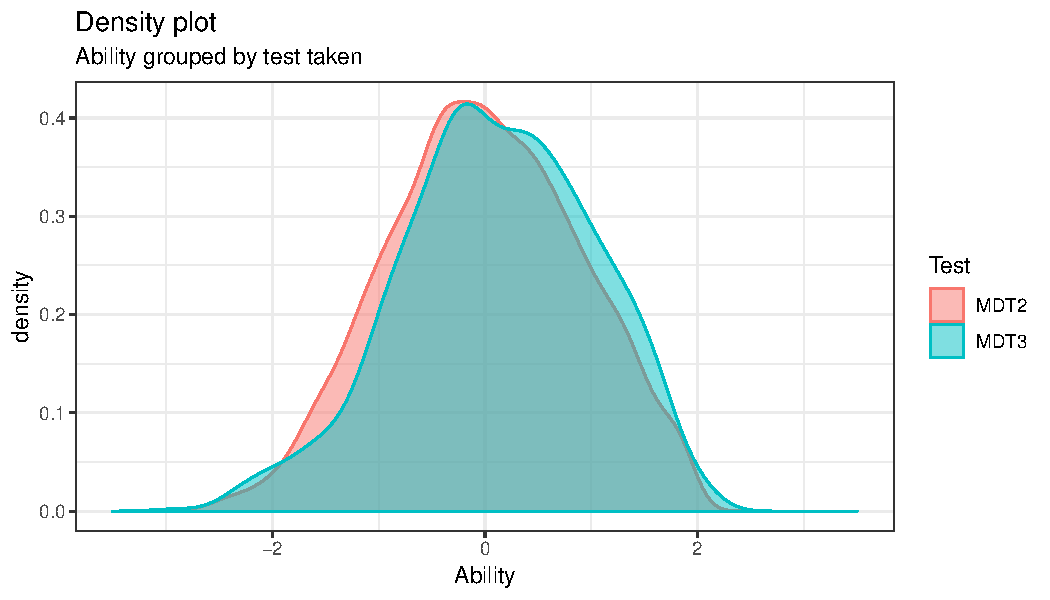
\includegraphics[width=\linewidth]{fig/IMPRV_CP_eap.pdf}
  \caption{\label{fig:IMPRV_CP_eap}Density plots of the estimated abilities of students grouped by test taken}
\end{figure}

\begin{table}[ht]
  \centering
  \begin{tabular}{rrrrrrrr}
    \hline
   & n & mean & sd & min & max & skew & kurtosis \\ 
    \hline
  MDT2 & 3248 & -0.02 & 0.90 & -2.77 & 1.82 & -0.07 & -0.48 \\ 
    MDT3 & 896 & 0.11 & 0.90 & -2.92 & 2.01 & -0.25 & -0.27 \\ 
     \hline
  \end{tabular}
  \caption{\label{tab:IMPRV_CP_eap_dsc}Basic descriptive statistics of the estimated abilities}
\end{table}

Although the results given by Model \texttt{MDT3-FCIP} and Model \texttt{MDT3-CP} are similar, there is a fundamental difference between these two models. Concurrent parameter (CP) calibration is the easiest approach to test equating because only one IRT model is fitted to a modified data set. However, the scale of the ability in CP calibration is a combination of the scales of ability of students from different years, which is not equal to any scale of ability from a specific year. If the test from a future year needs to be equated, the scale of the new model is not comparable with the existing one. Therefore, CP calibration is more of a one-off analysis. 

\section{Future MDT}

Improving MDT is a long-term task for the School of Mathematics. Based on the analyses in the chapter, a number of new criterion can be summarised, along with the criterion used in the summer 2017 project. 

\begin{itemize}
\item Item with low Major Info in Model \texttt{MDT3-FCIP} and Model \texttt{MDT3-CP} should be removed. 
\item Item which attains the maximum of its information function at positive value of ability should be kept. 
\end{itemize}

Therefore, in accordance with MDT3, we suggest removing Q15 and Q1. 


\chapter{Prediction of Outcomes}

To what extent do the results of mathematics diagnostic test (MDT) predict students' performance in mathematics courses since MDT changed in 2017, the performances of prediction of MDT2 and MDT3 will be compared in this chapter. 

% The results of mathematics diagnostic test (MDT) is used to determine the extent to which it can be used to predict the results of the exams of mathematics courses. Since MDT changed in the year of 2017, the performances of prediction of MDT2017 and MDT before 2017 will be compared in this chapter. 

\section{Introduction}

The raw data consists of the country of domicile based on fee status group, school, gender and assessment mark and grade in each course, and entry qualifications of the students. 

Students will be classified into four different groups of countries of domicile based on their fee status group. The four groups are Scotland, rest of the UK, rest of the European Union and other overseas countries. 

The classification of schools of the students are School of Mathematics, School of Informatics, School of Physics, School of Economics and other schools. 

In this project, only seven of the courses are considered, including Introduction to Linear Algebra (ILA), Calculus and its Applications (CAP), Proofs and Problem Solving (PPS), Mathematics for Physics 1 (MfP1), Accelerated Algebra and Calculus for Direct Entry (AAC), Accelerated Proofs and Problem Solving (APPS) and Several Variable Calculus and Differential Equations (SVCDE). Within these seven courses, ILA, CAP and PPS are Year 1 mathematics courses, MfP1 is the course for students who need extra mathematics practice, AAC and APPS are mathematics courses for Year 2 Direct Entry students and SVCDE is a Year 2 course for all mathematics students. 

According to the raw data of the course results, some special categories of assessment grades of students are recorded. Some students also made more than one attempt on a course. In order to reflect the actual outcomes after one year of study, the data need to be cleaned by the following procedures. 

\begin{enumerate}
\item Exclude the students with grade NO (non-assessed), WD (withdrawn) or NS (null sit with special circumstances); 
\item Keep only the results of the very first attempt in a course for each student; 
\item Map grade FF (force fail) onto grade E; 
\item Map grade ES (credits awarded with special circumstances) onto grade D; and
\item Treat grade AN (absent) as a grade ranked after grade H. 
\end{enumerate}

The entry qualifications of students includes Scottish Qualifications Authority (SQA) national qualifications, General Certificate of Education (GCE) Advanced Level (A-Levels), International Baccalaureate (IB) Diploma Programme and other qualifications. These qualifications are classified into three categories, corresponding to the recommendation of taking extra mathematics introductory courses or not, including

\begin{enumerate}[{Category} 1]
\item Strongly recommended to take extra mathematics courses, if a student has one of the following
  \begin{itemize}
  \item SQA Advanced Higher Mathematics at Grade C or below, or do not have Advanced Higher Mathematics; 
  \item A-Level Mathematics at Grade A AND do not have A-Level Further Mathematics, or have A-Level Mathematics at Grade B or below; 
  \item IB Mathematics SL. 
  \end{itemize}

\item Can take extra mathematics courses if a student wants more mathematics practice and has one of the following
  \begin{itemize}
  \item SQA Advanced Higher Mathematics at Grade B; 
  \item A-Level Mathematics at Grade A AND A-Level Further Mathematics at Grade A; 
  \item IB Mathematics HL at Grade H5. 
  \end{itemize}

\item Cannot take extra mathematics courses if a student has one of the following
  \begin{itemize}
  \item SQA Advanced Higher Mathematics at Grade A; 
  \item A-Level Mathematics at Grade A*; 
  \item IB Mathematics HL at Grade H6 or above. 
  \end{itemize}
\end{enumerate}

\begin{enumerate}[Unknown]
\item Should discuss with Personal Tutor, if a student has other qualifications. 
\end{enumerate}

In the sections below, different subsets of the clean data set may be used to perform analyses on corresponding groups of students.  

\section{Using diagnostic test}

According to the report last year, there exists a linear relationship between the three Year 1 courses (ILA, CAP and PPS) results and MDT scores, while the relationship between Year 2 course results and MDT scores is weaker \cite{lastyear}. In this section, the relationship between course results and MDT3 scores will be examined. The relationship between course results and the estimated abilities using GPCM is also investigated, as well as the performance of prediction of using abilities. 

\subsection{Linear regression}

The scatter plots of course results against MDT scores are shown in Figure~\ref{fig:REL_scatter_DT}. The blue lines in the plots are the fitted linear regression lines, with the grey shadow areas as the confidence interval. The correlation coefficients of the linear regressions are annotated. The points represent students who took both the course and MDT. 

It can be seen that the correlation coefficients for students taking MDT2 are generally higher than the correlation coefficients for students taking MDT2, implying that MDT3 provides better prediction of Year 1 course results. Within the three Year 1 courses, the correlation coefficients of ILA is the highest, followed by CAP and PPS. 

\begin{figure}[H]
  \centering
  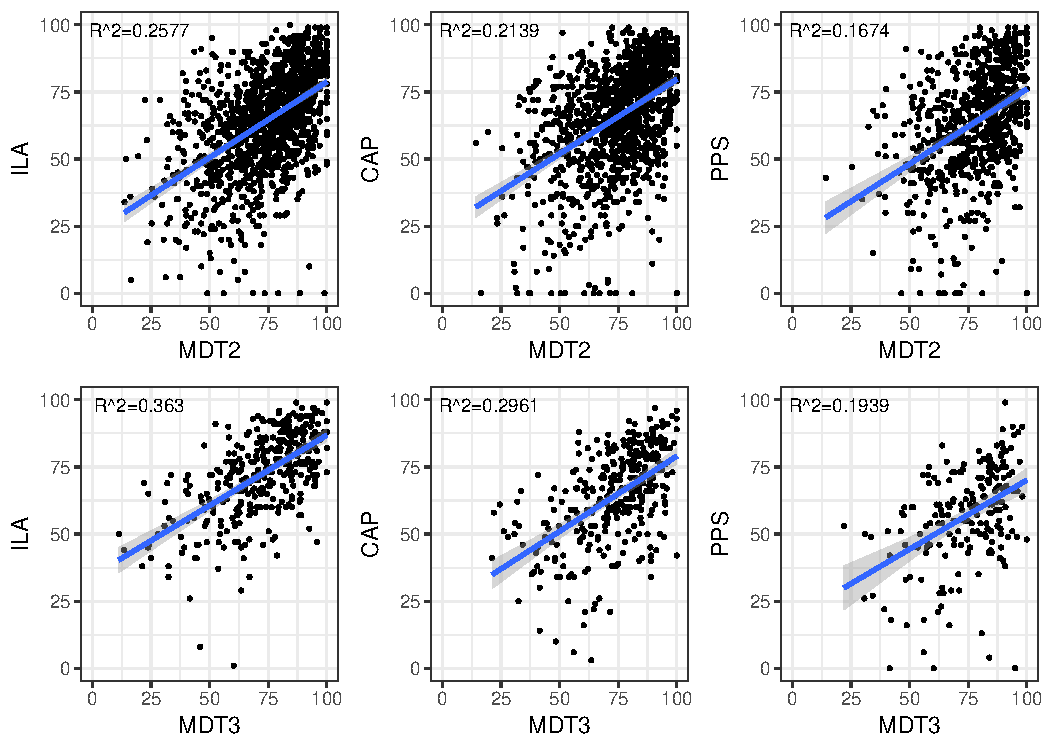
\includegraphics[width=\linewidth]{fig/REL_scatter_DT.pdf}
  \caption{\label{fig:REL_scatter_DT}Scatter plots of course results against MDT scores and linear regression lines, confidence intervals and correlation coefficients}
\end{figure}

The corresponding plots of course results against abilities estimated by EAP are shown in Figure~\ref{fig:REL_scatter_Ability}. The correlation coefficients of the linear regressions using estimated ability as the explanatory variable are lower for MDT2 than using MDT scores as the explanatory variable, while they are higher for MDT3. However, as discussed in Section~\ref{sec:IRT_EAP}, the estimated abilities come with confidence intervals which are affected by the upper limit of MDT scores, so the correlation investigated may not be accurate, especially for the above-average students. 

\begin{figure}[H]
  \centering
  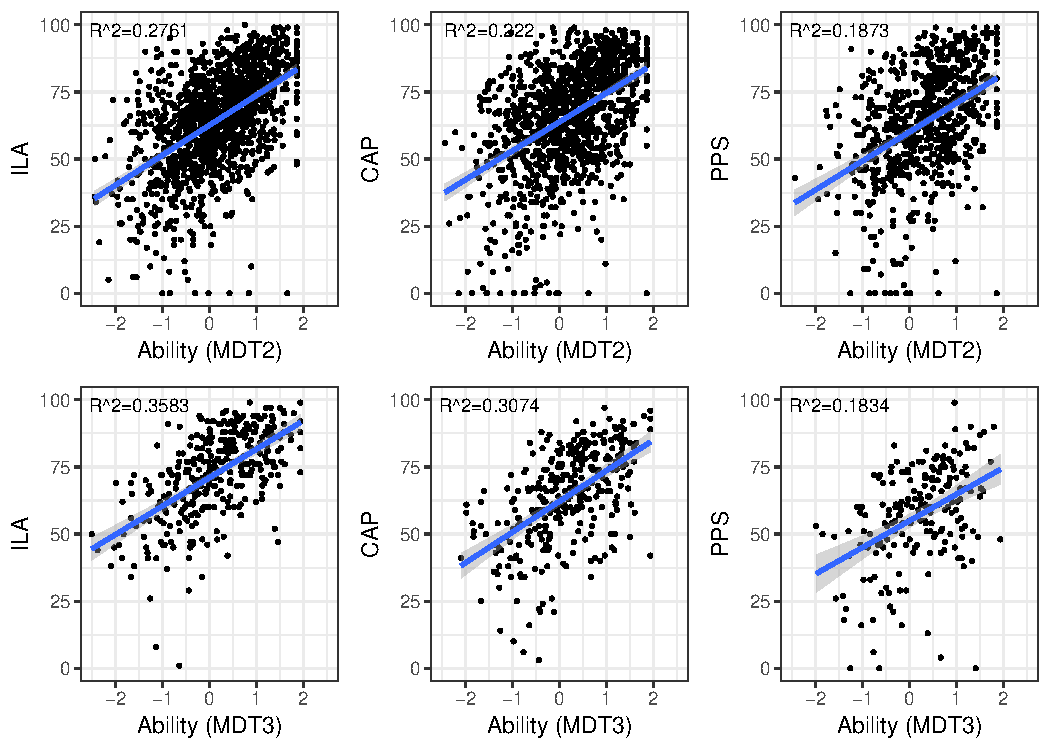
\includegraphics[width=\linewidth]{fig/REL_scatter_Ability.pdf}
  \caption{\label{fig:REL_scatter_Ability}Scatter plots of course results against estimated ability (EAP) and linear regression lines, confidence intervals and correlation coefficients}
\end{figure}

It should be noted that the correlation coefficients are lower than 0.6 whichever explanatory variable is used. A possible reason of this result is that MDT is taken before the teaching weeks start, so the course results may be influenced by other factors during the semester, including but not limited to the courses taught in the lectures, attendance of the tutorials and completion of assignments. 

\subsection{Visual representation}

To visualise the relationship between course results and MDT scores, we use stacked bar plots suggested by Bridgeman \cite{stackbar} and change width of the bars to be proportional that can represent the percentage of population in a certain group. Another advantage of using stacked bar plots is that the results can be easily interpreted by people with no knowledge about statistics. 

In Figure~\ref{fig:REL_ILAGrade_vs_MDT}, Figure~\ref{fig:REL_CAPGrade_vs_MDT} and Figure~\ref{fig:REL_PPSGrade_vs_MDT} are shown the stacked bar plots of the grades of Year 1 courses against different intervals of MDT scores. The population in these plots are the students who took the corresponding courses, ignoring their completion of MDT. The width of each bar represents the proportion of students who have MDT scores within the interval. The frequencies of the tiles are shown in Table~\ref{tab:REL_ILAGrade_vs_MDT}, Table~\ref{tab:REL_CAPGrade_vs_MDT} and Table~\ref{tab:REL_PPSGrade_vs_MDT}. 

\begin{figure}[H]
  \centering
  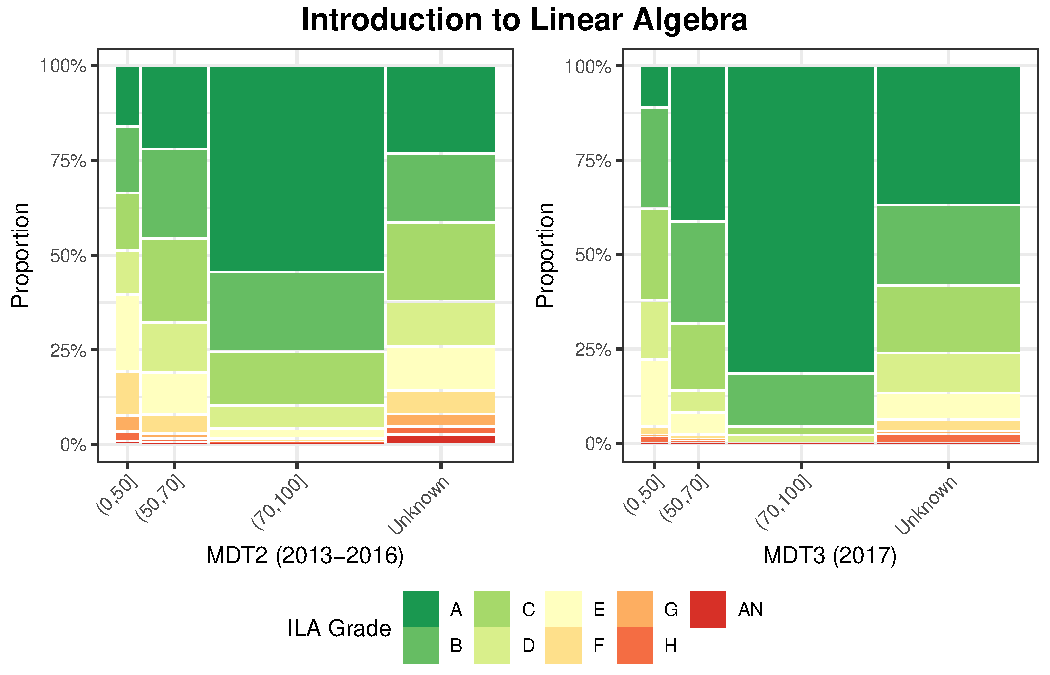
\includegraphics[width=\linewidth]{fig/REL_ILAGrade_vs_MDT.pdf}
  \caption{\label{fig:REL_ILAGrade_vs_MDT}Stacked bar plots of ILA grades against MDT scores with proportional width}
\end{figure}

\begin{table}[ht]
  \centering
  \begin{tabular}{r|cccc|c}
    \hline
    \multicolumn{6}{c}{\textbf{Introduction to Linear Algebra}} \\
    \hline
  2013-2016 & (0,50] & (50,70] & (70,100] & Unknown & Sum \\ 
    \hline
  A & 19 & 69 & 445 & 118 & 651 \\ 
    B & 21 & 74 & 171 & 94 & 360 \\ 
    C & 18 & 70 & 117 & 106 & 311 \\ 
    D & 14 & 41 & 49 & 61 & 165 \\ 
    E & 24 & 35 & 22 & 59 & 140 \\ 
    F & 14 & 16 & 7 & 32 & 69 \\ 
    G & 5 & 4 & 2 & 17 & 28 \\ 
    H & 3 & 3 & 0 & 11 & 17 \\ 
    AN & 1 & 2 & 4 & 13 & 20 \\ 
    \hline
    Sum & 119 & 314 & 817 & 511 & 1761 \\ 
     \hline
     \hline
    2017 & (0,50] & (50,70] & (70,100] & Unknown & Sum \\ 
      \hline
    A & 5 & 35 & 180 & 80 & 300 \\ 
      B & 12 & 23 & 31 & 46 & 112 \\ 
      C & 11 & 15 & 5 & 39 & 70 \\ 
      D & 7 & 5 & 5 & 23 & 40 \\ 
      E & 8 & 5 & 0 & 15 & 28 \\ 
      F & 1 & 1 & 0 & 7 & 9 \\ 
      G & 0 & 0 & 0 & 1 & 1 \\ 
      H & 1 & 1 & 0 & 6 & 8 \\ 
      AN & 0 & 0 & 0 & 0 & 0 \\ 
      \hline
      Sum & 45 & 85 & 221 & 217 & 568 \\ 
       \hline
  \end{tabular}
  \caption{\label{tab:REL_ILAGrade_vs_MDT}Contingency tables of corresponding frequencies}
\end{table}

\begin{figure}[H]
  \centering
  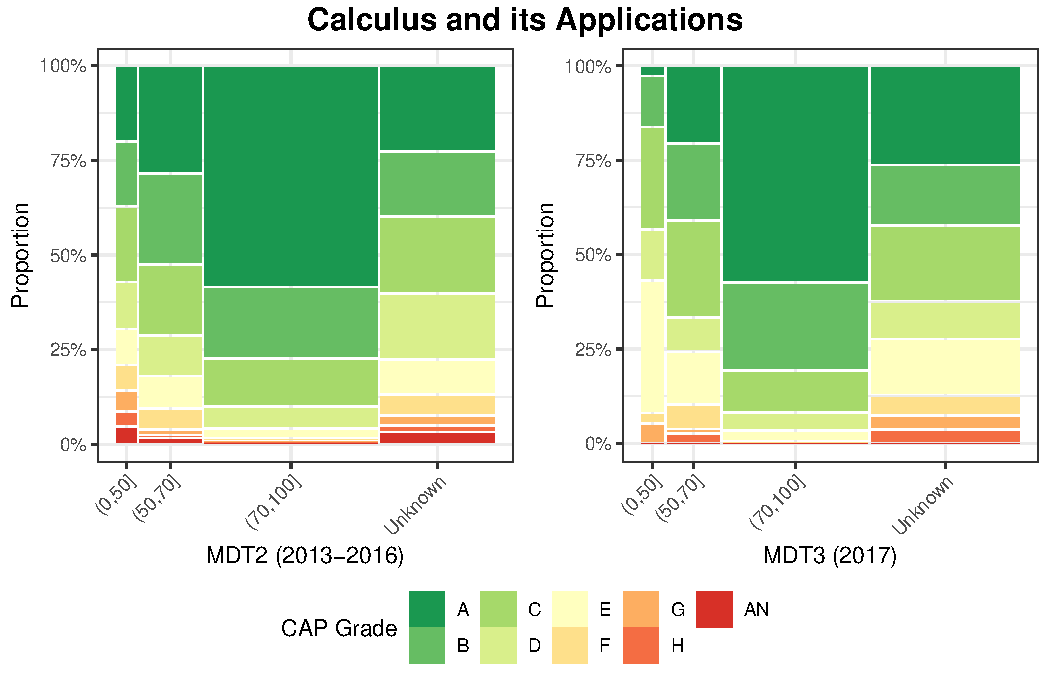
\includegraphics[width=\linewidth]{fig/REL_CAPGrade_vs_MDT.pdf}
  \caption{\label{fig:REL_CAPGrade_vs_MDT}Stacked bar plots of CAP grades against MDT scores with proportional width}
\end{figure}

\begin{table}[ht]
  \centering
  \begin{tabular}{r|cccc|c}
    \hline
    \multicolumn{6}{c}{\textbf{Calculus and its Applications}} \\
    \hline
  2013-2016 & (0,50] & (50,70] & (70,100] & Unknown & Sum \\ 
  \hline
  A & 21 & 82 & 456 & 118 & 677 \\ 
    B & 18 & 69 & 147 & 89 & 323 \\ 
    C & 21 & 54 & 99 & 107 & 281 \\ 
    D & 13 & 31 & 46 & 90 & 180 \\ 
    E & 10 & 25 & 19 & 49 & 103 \\ 
    F & 7 & 16 & 6 & 28 & 57 \\ 
    G & 6 & 4 & 1 & 14 & 25 \\ 
    H & 4 & 2 & 3 & 9 & 18 \\ 
    AN & 5 & 5 & 3 & 17 & 30 \\ 
    \hline
    Sum & 105 & 288 & 780 & 521 & 1694 \\ 
     \hline
     \hline
    2017 & (0,50] & (50,70] & (70,100] & Unknown & Sum \\ 
     \hline
   A & 1 & 16 & 118 & 56 & 191 \\ 
     B & 5 & 16 & 48 & 34 & 103 \\ 
     C & 10 & 20 & 23 & 43 & 96 \\ 
     D & 5 & 7 & 10 & 21 & 43 \\ 
     E & 13 & 11 & 6 & 32 & 62 \\ 
     F & 1 & 5 & 1 & 11 & 18 \\ 
     G & 2 & 1 & 0 & 8 & 11 \\ 
     H & 0 & 2 & 0 & 8 & 10 \\ 
     AN & 0 & 0 & 0 & 0 & 0 \\ 
    \hline
     Sum & 37 & 78 & 206 & 213 & 534 \\ 
      \hline
  \end{tabular}
  \caption{\label{tab:REL_CAPGrade_vs_MDT}Contingency tables of corresponding frequencies}
\end{table}

\begin{figure}[H]
  \centering
  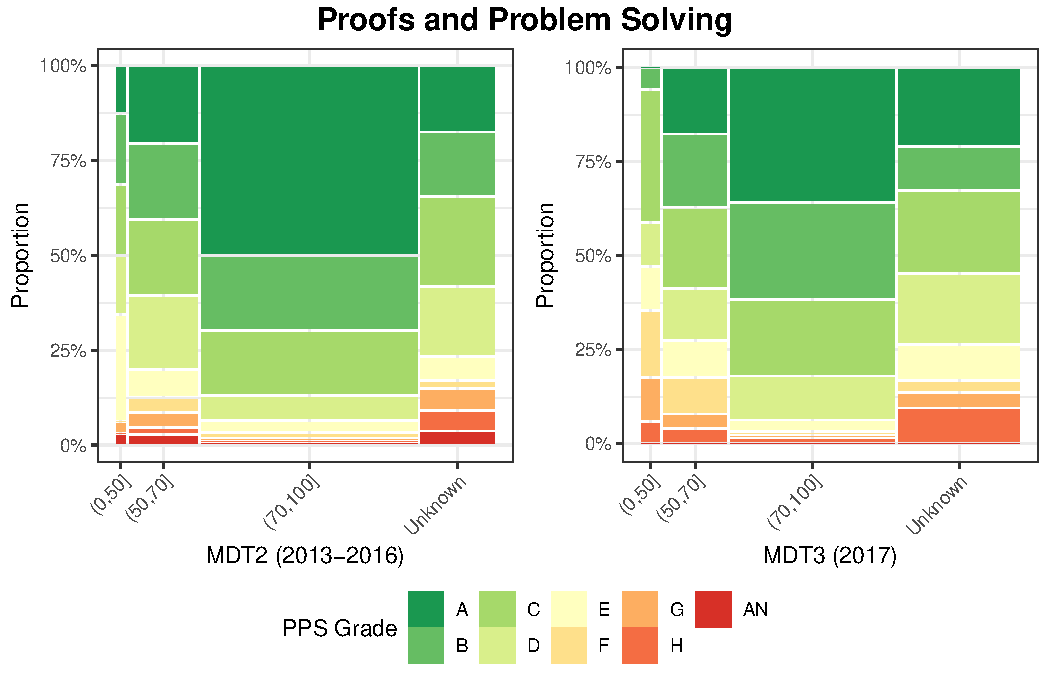
\includegraphics[width=\linewidth]{fig/REL_PPSGrade_vs_MDT.pdf}
  \caption{\label{fig:REL_PPSGrade_vs_MDT}Stacked bar plots of PPS grades against MDT scores with proportional width}
\end{figure}

\begin{table}[ht]
  \centering
  \begin{tabular}{r|cccc|c}
    \hline
    \multicolumn{6}{c}{\textbf{Proofs and Problem Solving}} \\
    \hline
  2013-2016 & (0,50] & (50,70] & (70,100] & Unknown & Sum \\ 
    \hline
  A & 4 & 36 & 268 & 33 & 341 \\ 
    B & 6 & 35 & 105 & 32 & 178 \\ 
    C & 6 & 35 & 92 & 45 & 178 \\ 
    D & 5 & 34 & 35 & 35 & 109 \\ 
    E & 9 & 13 & 17 & 12 & 51 \\ 
    F & 0 & 7 & 9 & 4 & 20 \\ 
    G & 1 & 7 & 3 & 11 & 22 \\ 
    H & 0 & 3 & 2 & 10 & 15 \\ 
    AN & 1 & 5 & 4 & 7 & 17 \\ 
    \hline
    Sum & 32 & 175 & 535 & 189 & 931 \\ 
    \hline
     \hline
    2017 & (0,50] & (50,70] & (70,100] & Unknown & Sum \\ 
    \hline
    A & 0 & 9 & 46 & 20 & 75 \\ 
      B & 1 & 10 & 33 & 11 & 55 \\ 
      C & 6 & 11 & 26 & 21 & 64 \\ 
      D & 2 & 7 & 15 & 18 & 42 \\ 
      E & 2 & 5 & 4 & 9 & 20 \\ 
      F & 3 & 5 & 1 & 3 & 12 \\ 
      G & 2 & 2 & 1 & 4 & 9 \\ 
      H & 1 & 2 & 2 & 9 & 14 \\ 
      AN & 0 & 0 & 0 & 0 & 0 \\ 
    \hline
      Sum & 17 & 51 & 128 & 95 & 291 \\ 
       \hline
  \end{tabular}
  \caption{\label{tab:REL_PPSGrade_vs_MDT}Contingency tables of corresponding frequencies}
\end{table}

Considering the students who took all three Year 1 courses, the stacked bar plots are shown in Figure~\ref{fig:REL_Y1Fs_vs_MDT_5070} and the corresponding frequencies are shown in Table~\ref{tab:REL_Y1Fs_vs_MDT_5070}. 

It can be seen that approximately 40\% of students who scored below 50 marks in MDT2, got more than 1 Grade D or below in the three Year 1 courses, while the percentage of students who scored above 70 drops to less than 10\%. The situations are similar for the students taking MDT3. 

\begin{figure}[H]
  \centering
  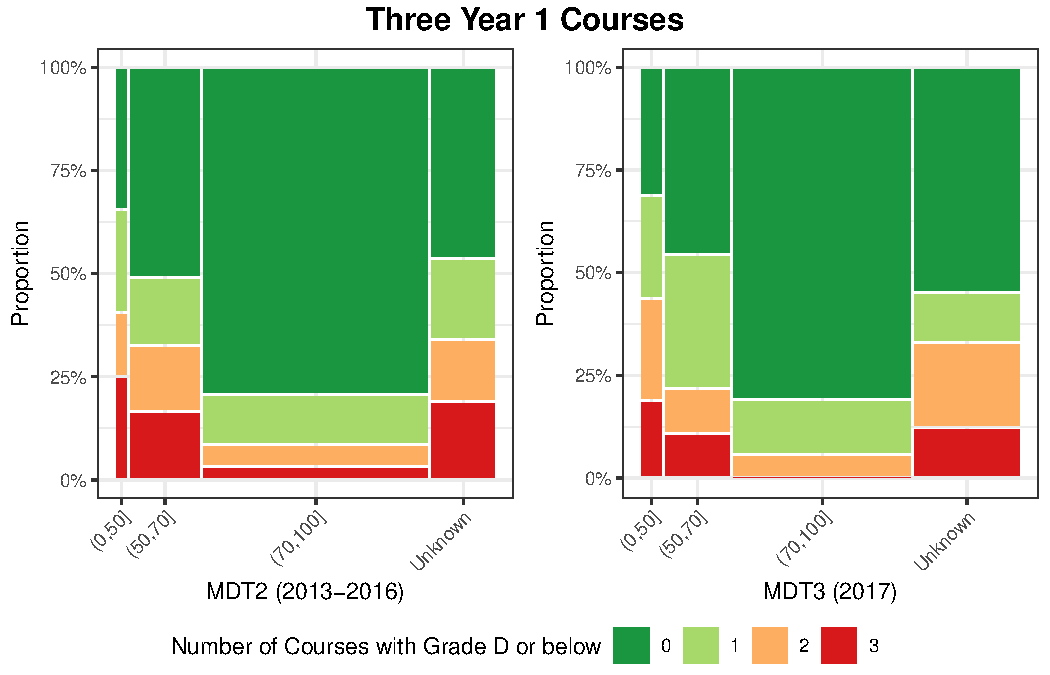
\includegraphics[width=\linewidth]{fig/REL_Y1Fs_vs_MDT_5070.pdf}
  \caption{\label{fig:REL_Y1Fs_vs_MDT_5070}Stacked bar plots of the number of courses with Grade D or below against MDT scores with proportional width}
\end{figure}

\begin{table}[ht]
  \centering
  \begin{tabular}{r|cccc|c}
    \hline
    \multicolumn{6}{c}{\textbf{Three Year 1 Courses}} \\
    \hline
  2013-2016 & (0,50] & (50,70] & (70,100] & Unknown & Sum \\ 
  \hline
  0 & 11 & 86 & 415 & 71 & 583 \\ 
    1 & 8 & 28 & 63 & 30 & 129 \\ 
    2 & 5 & 27 & 28 & 23 & 83 \\ 
    3 & 8 & 28 & 17 & 29 & 82 \\ 
    \hline
    Sum & 32 & 169 & 523 & 153 & 877 \\ 
     \hline
     \hline
    2017 & (0,50] & (50,70] & (70,100] & Unknown & Sum \\ 
    \hline
  0 & 5 & 21 & 98 & 40 & 164 \\ 
    1 & 4 & 15 & 16 & 9 & 44 \\ 
    2 & 4 & 5 & 7 & 15 & 31 \\ 
    3 & 3 & 5 & 0 & 9 & 17 \\ 
    \hline
    Sum & 16 & 46 & 121 & 73 & 256 \\ 
    \hline
  \end{tabular}
  \caption{\label{tab:REL_Y1Fs_vs_MDT_5070}Contingency tables of corresponding frequencies}
\end{table}

Since the three Year 1 courses are compulsory for students in the School of Mathematics, it is worth investigating the relationship between the number of courses with Grade D or below and MDT scores when the population is restricted to School of Mathematics students only. 

In Figure~\ref{fig:REL_Y1Fs_vs_MDT_maths} and Table~\ref{tab:REL_Y1Fs_vs_MDT_maths} are shown the stacked bar plots and the contingency tables of frequencies for students from School of Mathematics. 

It should be noted that the percentages of maths students attaining Grade C or above are slightly lower than the percentages of students from all schools. The report last year suggested that students from School of Mathematics had higher mean scores in MDT than the others \cite{lastyear}. These two findings imply that the factor of schools has higher influence on MDT scores rather than on Year 1 course results. 

\begin{figure}[H]
  \centering
  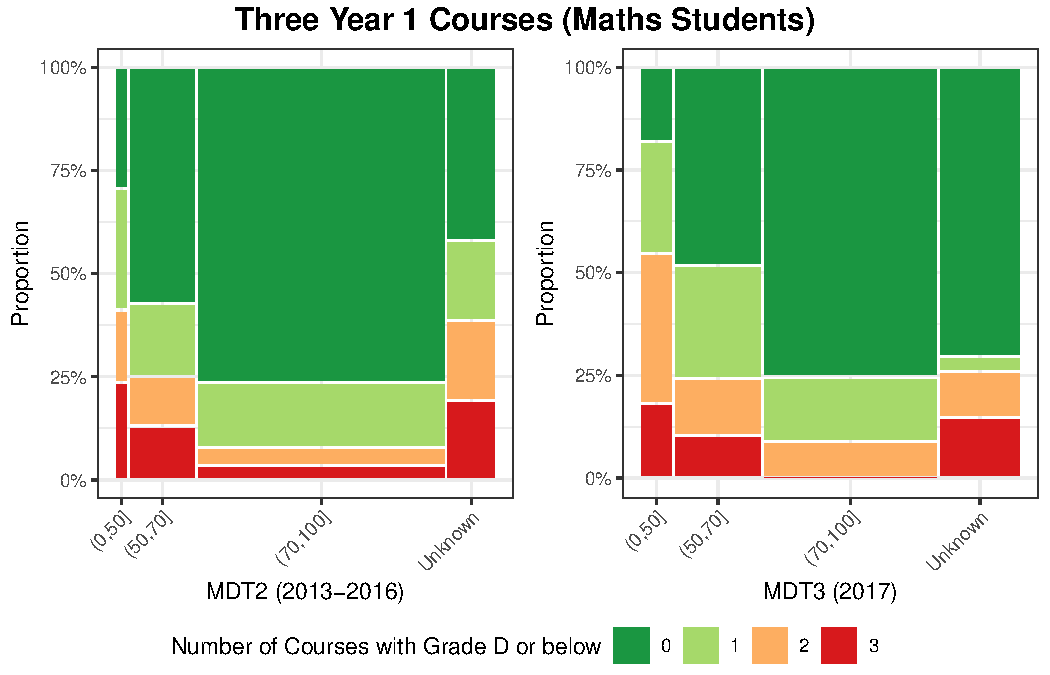
\includegraphics[width=\linewidth]{fig/REL_Y1Fs_vs_MDT_maths.pdf}
  \caption{\label{fig:REL_Y1Fs_vs_MDT_maths}Stacked bar plots of the number of courses with Grade D or below against MDT scores with proportional width}
\end{figure}

\begin{table}[ht]
  \centering
  \begin{tabular}{r|cccc|c}
    \hline
    \multicolumn{6}{c}{\textbf{Three Year 1 Courses (Maths Students)}} \\
    \hline
  2013-2016 & (0,50] & (50,70] & (70,100] & Unknown & Sum \\ 
    \hline
  0 & 5 & 48 & 233 & 26 & 312 \\ 
    1 & 5 & 15 & 48 & 12 & 80 \\ 
    2 & 3 & 10 & 13 & 12 & 38 \\ 
    3 & 4 & 11 & 11 & 12 & 38 \\
    \hline
    Sum & 17 & 84 & 305 & 62 & 468 \\ 
    \hline
     \hline
    2017 & (0,50] & (50,70] & (70,100] & Unknown & Sum \\ 
    \hline
    0 & 2 & 14 & 43 & 19 & 78 \\ 
      1 & 3 & 8 & 9 & 1 & 21 \\ 
      2 & 4 & 4 & 5 & 3 & 16 \\ 
      3 & 2 & 3 & 0 & 4 & 9 \\ 
    \hline
      Sum & 11 & 29 & 57 & 27 & 124 \\ 
       \hline
  \end{tabular}
  \caption{\label{tab:REL_Y1Fs_vs_MDT_maths}Contingency tables of corresponding frequencies}
\end{table}

Based on the analyses above, students who scored less than 50 marks in MDT should be strongly recommended to have extra mathematics practice, while those who scored higher than 70 marks do not need extra maths practice. For the students who scored between 50 and 70 marks, a subdivision may be needed. 

In Figure~\ref{fig:REL_Y1Fs_vs_MDT_506070} and Table~\ref{tab:REL_Y1Fs_vs_MDT_506070} are shown the stacked bar plots and contingency tables of the number of courses with Grade D or below against MDT scores where the range is divided with cut points 50, 60 and 70. 

The difference in proportions of the numbers of Grade Ds or below for students who scored between 50 and 60 and students who scored between 60 and 70 varies across the years. In 2017, the percentage of students with 3 Grade Ds or below, given MDT scores between 60 and 70, is even higher than those scoring between 50 and 60 marks in MDT. This may due to the higher difficulties in MDT3 and the small sample size. Considering that for students with 50 to 70 marks in MDT, there are approximately 25\% of students with more than 1 Grade D or below in the three Year 1 courses, given their MDT scores which are between 50 and 60, these students should be suggested to have extra maths practice. 

\begin{figure}[H]
  \centering
  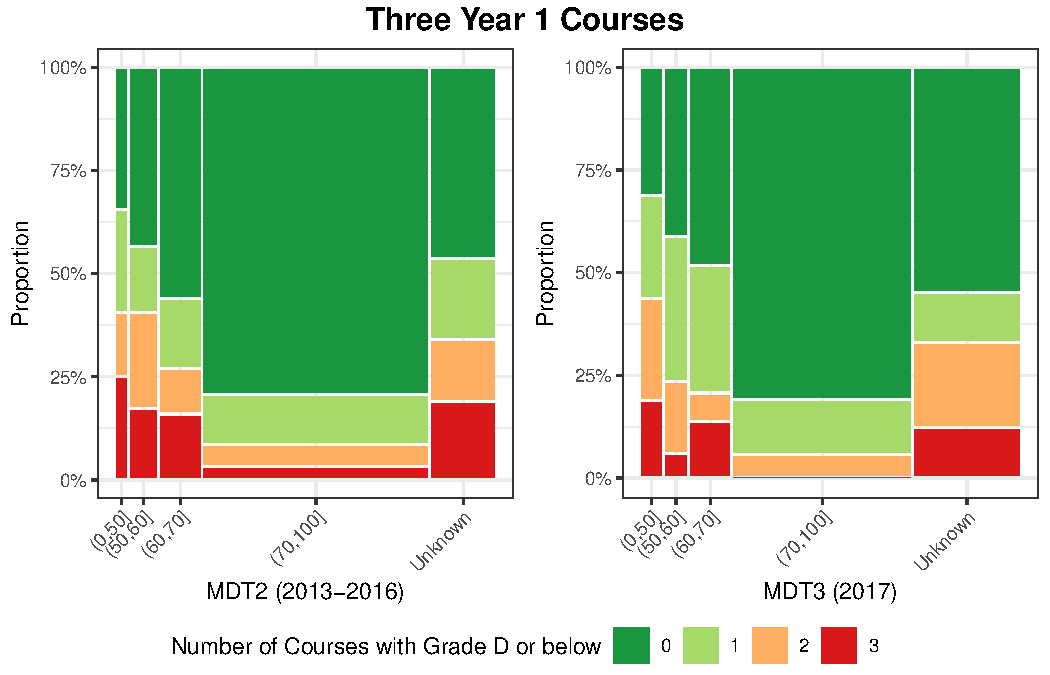
\includegraphics[width=\linewidth]{fig/REL_Y1Fs_vs_MDT_506070.pdf}
  \caption{\label{fig:REL_Y1Fs_vs_MDT_506070}Stacked bar plots of the number of courses with Grade D or below against MDT scores with proportional width}
\end{figure}

\begin{table}[ht]
  \centering
  \begin{tabular}{r|ccccc|c}
    \hline
    \multicolumn{7}{c}{\textbf{Three Year 1 Courses}} \\
    \hline
  2013-2016 & (0,50] & (50,60] & (60,70] & (70,100] & Unknown & Sum \\ 
    \hline
  0 & 11 & 30 & 56 & 415 & 71 & 583 \\ 
    1 & 8 & 11 & 17 & 63 & 30 & 129 \\ 
    2 & 5 & 16 & 11 & 28 & 23 & 83 \\ 
    3 & 8 & 12 & 16 & 17 & 29 & 82 \\ 
    \hline
    Sum & 32 & 69 & 100 & 523 & 153 & 877 \\ 
    \hline
    \hline
    2017 & (0,50] & (50,60] & (60,70] & (70,100] & Unknown & Sum \\ 
     \hline
   0 & 5 & 7 & 14 & 98 & 40 & 164 \\ 
     1 & 4 & 6 & 9 & 16 & 9 & 44 \\ 
     2 & 4 & 3 & 2 & 7 & 15 & 31 \\ 
     3 & 3 & 1 & 4 & 0 & 9 & 17 \\ 
    \hline
     Sum & 16 & 17 & 29 & 121 & 73 & 256 \\ 
      \hline
  \end{tabular}
  \caption{\label{tab:REL_Y1Fs_vs_MDT_506070}Contingency tables of corresponding frequencies}
\end{table}

\section{Using entry qualifications}

The entry qualifications of students may reflect their ability in high school mathematics, which might be correlated to the MDT scores and the Year 1 mathematics course results. 

The raw data only consists of the entry qualifications for students from 2017, but some of these students are from other schools and took none of the Year 1 mathematics courses (ILA, CAP, PPS) or Year 2 mathematics courses for direct entry students (AAC, APPS). Therefore, a subset of these students should be used in the analyses. 

In Table~\ref{tab:REL_freq_qual} are shown the frequency table of the categories of the students who took at least one of five courses (ILA, CAP, PPS, AAC, APPS). More than 40\% of these students have unknown entry qualifications. 

\begin{table}[ht]
  \centering
  \begin{tabular}{rrrr|r}
    \hline
  Cat1 & Cat2 & Cat3 & Unknown & Sum \\ 
    \hline
  120 & 48 & 245 & 295 & 708 \\ 
     \hline
  \end{tabular}
  \caption{\label{tab:REL_freq_qual}Frequency of students entry qualifications}
\end{table}

Within the students with unknown entry qualifications, over 70\% of them are from outside of the UK (Table~\ref{tab:REL_freq_qual_vs_region}). 

\begin{table}[ht]
  \centering
  \begin{tabular}{r|rrrr|r}
    \hline
   & EU & Overseas & RUK & Scotland & Sum \\ 
    \hline
  Known & 31 & 78 & 136 & 168 & 413 \\ 
    Unknown & 90 & 118 & 62 & 25 & 295 \\ 
    \hline
    Sum & 121 & 196 & 198 & 193 & 708 \\ 
     \hline
  \end{tabular}
  \caption{\label{tab:REL_freq_qual_vs_region}Contingency table of entry qualifications against regions}
\end{table}

\subsection{Visual representation}

The stacked bar plots of the grades of Year 1 courses against different entry qualifications with proportional width are shown in Figure~\ref{fig:REL_Grade_vs_Qual}. Comparing with the plots for 2017 in Figure~\ref{fig:REL_ILAGrade_vs_MDT}, Figure~\ref{fig:REL_CAPGrade_vs_MDT} and Figure~\ref{fig:REL_PPSGrade_vs_MDT}, the proportions of students getting higher grade given Category 1 entry qualifications are higher than those scoring below 50 marks in MDT. 

\begin{figure}[H]
  \centering
  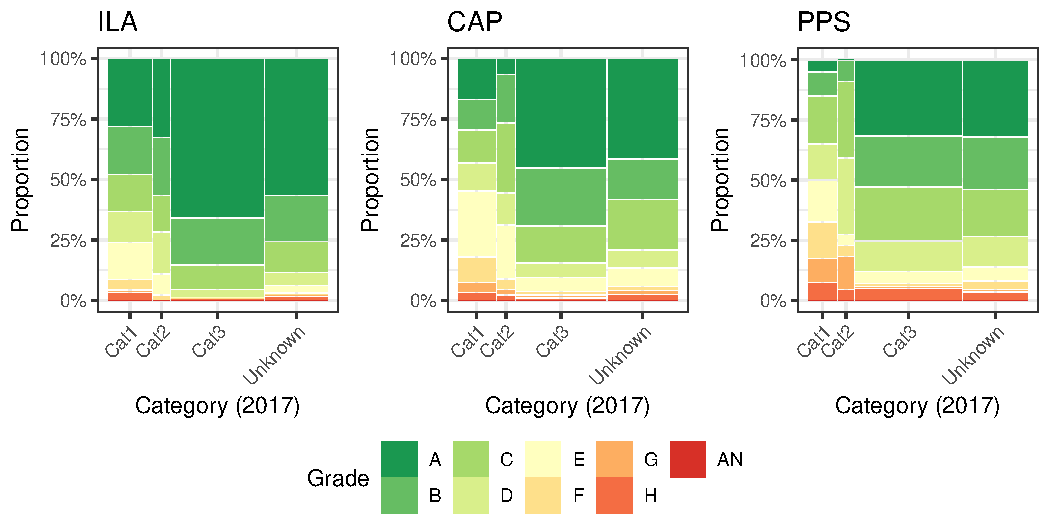
\includegraphics[width=\linewidth]{fig/REL_Grade_vs_Qual.pdf}
  \caption{\label{fig:REL_Grade_vs_Qual}Stacked bar plots of grades of Year 1 courses against entry qualifications with proportional width}
\end{figure}

The corresponding contingency tables of frequencies are shown in Table~\ref{tab:REL_ILAGrade_vs_Qual}, Table~\ref{tab:REL_CAPGrade_vs_Qual} and Table~\ref{tab:REL_PPSGrade_vs_Qual}. 

\begin{table}[H]
  \centering
  \begin{tabular}{r|cccc|c}
    \hline
    \multicolumn{6}{c}{\textbf{Introduction to Linear Algebra}} \\
    \hline
   2017 & Cat1 & Cat2 & Cat3 & Unknown & Sum \\ 
    \hline
  A & 33 & 15 & 159 & 93 & 300 \\ 
    B & 23 & 11 & 47 & 31 & 112 \\ 
    C & 18 & 7 & 24 & 21 & 70 \\ 
    D & 15 & 8 & 8 & 9 & 40 \\ 
    E & 18 & 4 & 1 & 5 & 28 \\ 
    F & 5 & 1 & 1 & 2 & 9 \\ 
    G & 1 & 0 & 0 & 0 & 1 \\ 
    H & 4 & 0 & 1 & 3 & 8 \\ 
    AN & 0 & 0 & 0 & 0 & 0 \\ 
    \hline
    Sum & 117 & 46 & 241 & 164 & 568 \\ 
     \hline
  \end{tabular}
  \caption{\label{tab:REL_ILAGrade_vs_Qual}Contingency table of corresponding frequencies}
\end{table}

\begin{table}[H]
  \centering
  \begin{tabular}{r|cccc|c}
    \hline
    \multicolumn{6}{c}{\textbf{Calculus and its Applications}} \\
    \hline
   2017 & Cat1 & Cat2 & Cat3 & Unknown & Sum \\ 
    \hline
  A & 16 & 3 & 100 & 72 & 191 \\ 
    B & 12 & 9 & 53 & 29 & 103 \\ 
    C & 13 & 13 & 34 & 36 & 96 \\ 
    D & 11 & 6 & 13 & 13 & 43 \\ 
    E & 26 & 10 & 13 & 13 & 62 \\ 
    F & 10 & 2 & 3 & 3 & 18 \\ 
    G & 4 & 1 & 3 & 3 & 11 \\ 
    H & 3 & 1 & 2 & 4 & 10 \\ 
    AN & 0 & 0 & 0 & 0 & 0 \\ 
    \hline
    Sum & 95 & 45 & 221 & 173 & 534 \\ 
     \hline
  \end{tabular}
  \caption{\label{tab:REL_CAPGrade_vs_Qual}Contingency table of corresponding frequencies}
\end{table}

\begin{table}[H]
  \centering
  \begin{tabular}{r|cccc|c}
    \hline
    \multicolumn{6}{c}{\textbf{Proofs and Problem Solving}} \\
    \hline
   2017 & Cat1 & Cat2 & Cat3 & Unknown & Sum \\ 
    \hline
  A & 2 & 0 & 45 & 28 & 75 \\ 
    B & 4 & 2 & 30 & 19 & 55 \\ 
    C & 8 & 7 & 32 & 17 & 64 \\ 
    D & 6 & 7 & 18 & 11 & 42 \\ 
    E & 7 & 1 & 7 & 5 & 20 \\ 
    F & 6 & 1 & 2 & 3 & 12 \\ 
    G & 4 & 3 & 1 & 1 & 9 \\ 
    H & 3 & 1 & 7 & 3 & 14 \\ 
    AN & 0 & 0 & 0 & 0 & 0 \\ 
    \hline
    Sum & 40 & 22 & 142 & 87 & 291 \\ 
     \hline
  \end{tabular}
  \caption{\label{tab:REL_PPSGrade_vs_Qual}Contingency table of corresponding frequencies}
\end{table}

Considering the students who took all three Year 1 courses, the stacked bar plots are shown in Figure~\ref{fig:REL_Y1Fs_vs_Qual} and the corresponding frequencies are shown in Table~\ref{tab:REL_Y1Fs_vs_Qual}. 

It is similar to the findings in Figure~\ref{fig:REL_Grade_vs_Qual} that the proportion of students getting 0 Grade Ds in the three courses is higher and the proportion of getting more than 1 Grade Ds is higher, for the group of students with Category 1 entry qualifications than the group of students with lower than 50 marks in MDT. The group of students with Category 2 entry qualifications are worse than the group of students with 50 to 70 marks in MDT. The group of students with Category 3 entry qualifications are slightly worse than the group of students with higher than 70 marks in MDT. Interestingly, the students with unknown category of entry qualifications performed even better than those with Category 3, which may due to the higher proportion of the overseas students. 

\begin{figure}[H]
  \centering
  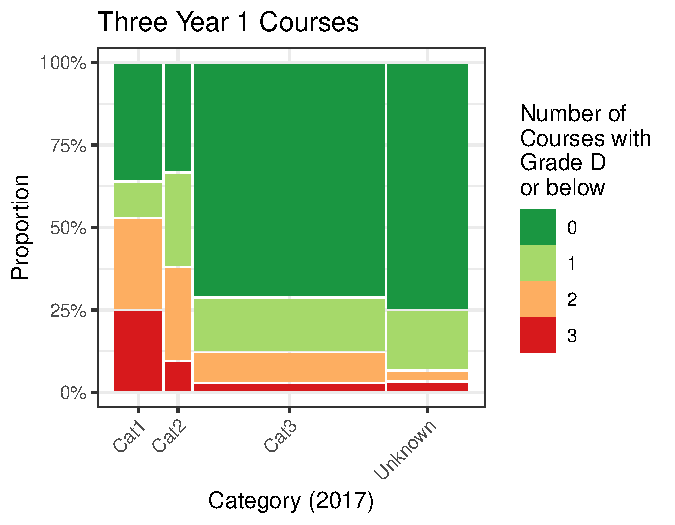
\includegraphics[width=.7\linewidth]{fig/REL_Y1Fs_vs_Qual.pdf}
  \caption{\label{fig:REL_Y1Fs_vs_Qual}Stacked bar plots of the number of courses with Grade D or below against entry qualifications with proportional width}
\end{figure}

\begin{table}[H]
  \centering
  \begin{tabular}{r|cccc|c}
    \hline
    \multicolumn{6}{c}{\textbf{Three Year 1 Courses}} \\
    \hline
   2017 & Cat1 & Cat2 & Cat3 & Unknown & Sum \\ 
    \hline
  0 & 13 & 7 & 99 & 45 & 164 \\ 
    1 & 4 & 6 & 23 & 11 & 44 \\ 
    2 & 10 & 6 & 13 & 2 & 31 \\ 
    3 & 9 & 2 & 4 & 2 & 17 \\ 
    \hline
    Sum & 36 & 21 & 139 & 60 & 256 \\ 
     \hline
  \end{tabular}
  \caption{\label{tab:REL_Y1Fs_vs_Qual}Contingency table of corresponding frequencies}
\end{table}

In Figure~\ref{fig:REL_Y1Fs_vs_Qual_maths} and Table~\ref{tab:REL_Y1Fs_vs_Qual_maths} are shown the stacked bar plots and the contingency table of frequencies for students from the School of Mathematics. The performances of maths students in these three categories seem to be worse than the three groups using intervals of MDT scores. 

\begin{figure}[H]
  \centering
  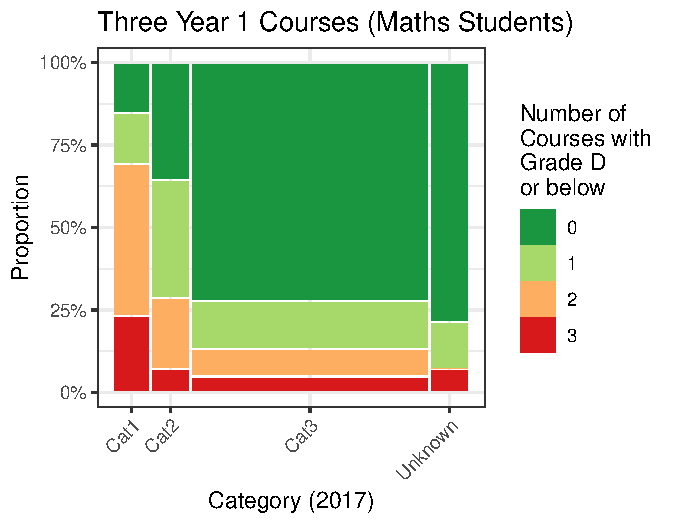
\includegraphics[width=.7\linewidth]{fig/REL_Y1Fs_vs_Qual_maths.pdf}
  \caption{\label{fig:REL_Y1Fs_vs_Qual_maths}Stacked bar plots of the number of courses with Grade D or below against entry qualifications with proportional width}
\end{figure}

\begin{table}[H]
  \centering
  \begin{tabular}{r|cccc|c}
    \hline
    \multicolumn{6}{c}{\textbf{Three Year 1 Courses (Maths Students)}} \\
    \hline
   2017 & Cat1 & Cat2 & Cat3 & Unknown & Sum \\ 
    \hline
  0 & 2 & 5 & 60 & 11 & 78 \\ 
    1 & 2 & 5 & 12 & 2 & 21 \\ 
    2 & 6 & 3 & 7 & 0 & 16 \\ 
    3 & 3 & 1 & 4 & 1 & 9 \\ 
    \hline
    Sum & 13 & 14 & 83 & 14 & 124 \\ 
     \hline
  \end{tabular}
  \caption{\label{tab:REL_Y1Fs_vs_Qual_maths}Contingency table of corresponding frequencies}
\end{table}

\subsection{Comparison with diagnostic test}

The relationship between MDT scores and entry qualifications is also of interest. Since the MDT scores or entry qualifications of some students are not recorded in the raw data, only the students who have MDT scores and took at least one of the five courses are considered. In Figure~\ref{fig:REL_MDT_vs_Qual} and Table~\ref{tab:REL_MDT_vs_Qual} are shown the stacked bar plots and contingency table of the frequencies of different intervals of MDT scores against different categories of entry qualifications. 

It can be seen that only a half of students with Category 1 entry qualifications scored higher than 60 marks in MDT, while there are only approximately 10\% of students with Category 3 entry qualifications scoring lower than 60 marks in MDT. 

\begin{figure}[H]
  \centering
  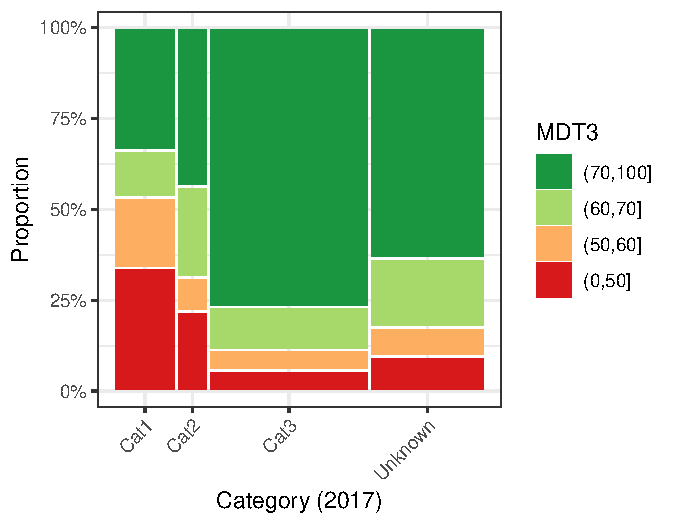
\includegraphics[width=.7\linewidth]{fig/REL_MDT_vs_Qual.pdf}
  \caption{\label{fig:REL_MDT_vs_Qual}Stacked bar plots of MDT scores against entry qualifications with proportional width}
\end{figure}

\begin{table}[H]
  \centering
  \begin{tabular}{r|cccc|c}
    \hline
   2017 & Cat1 & Cat2 & Cat3 & Unknown & Sum \\ 
   \hline
   (70,100] & 21 & 14 & 123 & 73 & 231 \\ 
     (60,70] & 8 & 8 & 19 & 22 & 57 \\ 
     (50,60] & 12 & 3 & 9 & 9 & 33 \\ 
     (0,50] & 21 & 7 & 9 & 11 & 48 \\ 
    \hline
     Sum & 62 & 32 & 160 & 115 & 369 \\ 
      \hline
  \end{tabular}
  \caption{\label{tab:REL_MDT_vs_Qual}Contingency table of corresponding frequencies}
\end{table}

\section{\label{sec:stackbar_binclf}Combining two}

Based on the previous analyses, MDT scores can be used to refine the recommendation to students about whether they need extra mathematics practice. 

Table~\ref{tab:REL_refine_all} shows the detailed categorisations of recommendation to students. The population is the students took all three Year 1 courses. 

\begin{table}[ht]
  \centering
  \begin{tabular}{r|ccccc}
    \hline
    & Cat1 & Cat2 & Cat3 & Unknown \\ 
   \hline
   (70,100] & Cat1+ & Cat2+ & Cat3+ & Unknown  \\ 
     (60,70] & Cat1- & Cat2+ & Cat3+ & Unknown  \\ 
     (50,60] & Cat1- & Cat2- & Cat3+ & Unknown  \\ 
     (0,50] & Cat1- & Cat2- & Cat3- & Unknown  \\ 
    Unknown & Cat1- & Cat2- & Cat3+ & Unknown \\
      \hline
  \end{tabular}
  \caption{\label{tab:REL_refine_all}Detailed categories of recommendation}
\end{table}

In Figure~\ref{fig:REL_Y1Fs_vs_NewCat_all} and Table~\ref{tab:REL_Y1Fs_vs_NewCat} are shown the stacked bar plot of the number of courses with Grade D or below against different refined categories of recommendation. The population size for each category are relatively small, so the proportions may not be sensible. 

\begin{figure}[H]
  \centering
  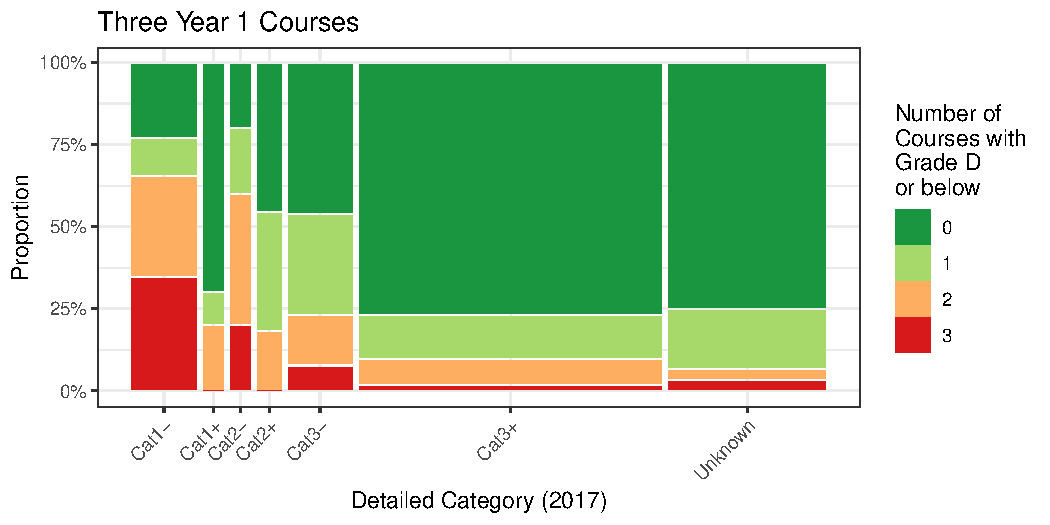
\includegraphics[width=\linewidth]{fig/REL_Y1Fs_vs_NewCat_all.pdf}
  \caption{\label{fig:REL_Y1Fs_vs_NewCat_all}Stacked bar plots of the number of courses with Grade D or below against refined categories of recommendation}
\end{figure}

\begin{table}[H]
  \centering
  \begin{tabular}{r|ccccccc|c}
    \hline
    \multicolumn{9}{c}{\textbf{Three Year 1 Courses}} \\
    \hline
   2017 & Cat1- & Cat1+ & Cat2- & Cat2+ & Cat3- & Cat3+ & Unknown & Sum \\ 
    \hline
  0 & 6 & 7 & 2 & 5 & 12 & 87 & 45 & 164 \\ 
    1 & 3 & 1 & 2 & 4 & 8 & 15 & 11 & 44 \\ 
    2 & 8 & 2 & 4 & 2 & 4 & 9 & 2 & 31 \\ 
    3 & 9 & 0 & 2 & 0 & 2 & 2 & 2 & 17 \\ 
    \hline
    Sum & 26 & 10 & 10 & 11 & 26 & 113 & 60 & 256 \\ 
     \hline
  \end{tabular}
  \caption{\label{tab:REL_Y1Fs_vs_NewCat_all}Contingency table of corresponding frequencies}
\end{table}

Table~\ref{tab:REL_refine} shows the refined categories recommendation to students, where `Cat-' represents `recommended to take extra maths course' and `Cat+' represents `not recommended to take extra maths course'. The population is the students took all three Year 1 courses. 

\begin{table}[ht]
  \centering
  \begin{tabular}{r|ccccc}
    \hline
    & Cat1 & Cat2 & Cat3 & Unknown \\ 
   \hline
   (70,100] & Cat+ & Cat+ & Cat+ & Cat+  \\ 
     (60,70] & Cat- & Cat+ & Cat+ & Cat+  \\ 
     (50,60] & Cat- & Cat- & Cat+ & Cat-  \\ 
     (0,50] & Cat- & Cat- & Cat- & Cat-  \\ 
    Unknown & Cat- & Cat- & Cat+ & Unknown \\
      \hline
  \end{tabular}
  \caption{\label{tab:REL_refine}Refined categories of recommendation}
\end{table}

In Figure~\ref{fig:REL_Y1Fs_vs_NewCat} and Table~\ref{tab:REL_Y1Fs_vs_NewCat} are shown the stacked bar plot of the number of courses with Grade D or below against different refined categories of recommendation. 

\begin{figure}[H]
  \centering
  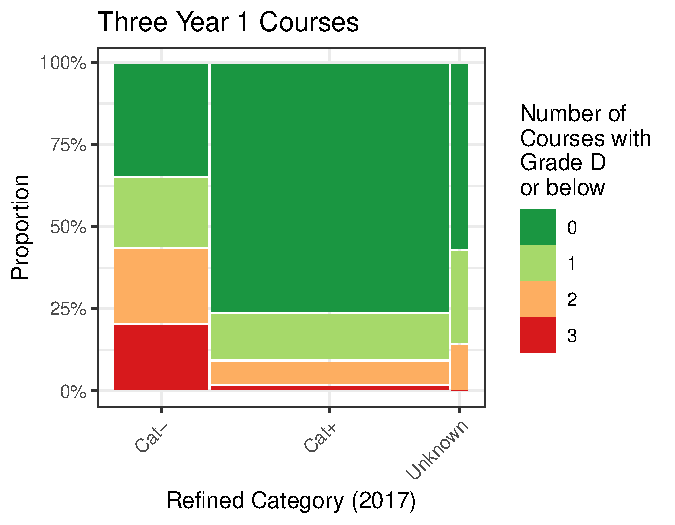
\includegraphics[width=.7\linewidth]{fig/REL_Y1Fs_vs_NewCat.pdf}
  \caption{\label{fig:REL_Y1Fs_vs_NewCat}Stacked bar plots of the number of courses with Grade D or below against refined categories of recommendation}
\end{figure}

\begin{table}[H]
  \centering
  \begin{tabular}{r|ccc|c}
    \hline
    \multicolumn{5}{c}{\textbf{Three Year 1 Courses}} \\
    \hline
   2017 & Cat- & Cat+ & Unknown & Sum \\ 
    \hline
  0 & 24 & 132 & 8 & 164 \\ 
    1 & 15 & 25 & 4 & 44 \\ 
    2 & 16 & 13 & 2 & 31 \\ 
    3 & 14 & 3 & 0 & 17 \\ 
    \hline
    Sum & 69 & 173 & 14 & 256 \\ 
     \hline
  \end{tabular}
  \caption{\label{tab:REL_Y1Fs_vs_NewCat}Contingency table of corresponding frequencies}
\end{table}

\subsubsection{\label{subsec:cm}Binary classification}

To evaluate a binary classifier that classifies the elements into two classes, a special kind of contingency table with two dimensions (`true condition' and `predicted condition') and identical sets of classes (`positive' and `negative') in both dimensions is used as a visualisation of the performance of the classifier \cite{cm}. This special kind of contingency table is called confusion matrix, which is summarised in Table~\ref{tab:cm}. 

\begin{table}[ht]
  \centering
  \begin{tabular}{c|c|c|c}
    \hline
    \multicolumn{2}{c|}{} & \multicolumn{2}{c}{Predicted Condition} \\ 
    \cline{3-4}
    \multicolumn{2}{c|}{} & Positive & Negative \\ 
    \hline
  True & Positive & True Positive (TP) & False Negative (FN) \\ 
    \cline{2-4}
    Condition & Negative & False Positive (FN) & True Negative (TN) \\ 
     \hline
  \end{tabular}
  \caption{\label{tab:cm}Confusion matrix}
\end{table}

In our context, if students with more than 1 Grade D are considered to be (true) at-risk (positive) and the others are considered not to be at-risk, the refined categories can be used as a predictor to the courses result, where Cat- represents predicted positive and Cat+ represents predicted negative. 

The accuracy of the classifier, i.e. the proportion of correct classifications, is calculated by

$$ACC = \frac{TP+TN}{TP+FN+TN+FP} \text{. }$$

\noindent
However, accuracy is not a reliable metric and gives misleading results when the numbers of observations in different classes vary greatly \cite{ACClimit}. Alternatively, two fundamental statistics that are independent on prevalence (proportion of true conditional positive), Sensitivity (also known as True Positive Rate, TPR) and Specificity (also known as True Negative Rate, TNR) can used as measures of the performance of a binary classifier. Sensitivity or True Positive Rate is calculated by 

$$TPR = \frac{TP}{TP+FN} \text{, }$$

\noindent
and Specificity or True Negative Rate is calculated by 

$$TNR = \frac{TN}{TN+FP} \text{. }$$

When we are assessing how the results of MDT predict students' performance in mathematics courses, we are aiming at identifying more students who are at risk (higher TPR) while avoiding decreasing the number of students that are classified into not-at-risk correctly (lower TNR). 

The confusion matrix of this classifier that combines MDT results and entry qualifications is shown in Table~\ref{tab:REL_cm_NewCat}. 

\begin{table}[ht]
  \centering
  \begin{tabular}{rcc}
    \hline
   & Predicted At-Risk & Predicted Not-At-Risk \\ 
    \hline
  True At-Risk & 30 & 16 \\ 
    True Not-At-Risk & 39 & 157 \\ 
     \hline
  \end{tabular}
  \caption{\label{tab:REL_cm_NewCat}Confusion matrix of refined categories classification}
\end{table}

The accuracy of this classification method is calculated by 

$$ACC = \frac{TP+TN}{TP+FN+TN+FP} = \frac{30+157}{30+16+39+157} = 77.2\% \text{, }$$

\noindent
and the sensitivity is calculated by 

$$TPR = \frac{TP}{TP+FN} = \frac{30}{30+16} = 65.22\% \text{. }$$

\section{Extra maths courses}

In previous years, students from School of Mathematics who scored lower than 65 marks in MDT were suggested to take Mathematics for Physics 1 (MfP1) as the extra mathematics practice. This section is aimed at examining whether MfP1 helped improved the results of other mathematics courses. 

The scatter plots of course results in the three Year 1 courses against MDT scores are shown in Figure~\ref{fig:REL_scatter_MfP1}. In these plots, students are grouped by their selections of MfP1. The blue points does not form a cluster separated from the red points, implying that taking MfP1 might not do great help to students. 

\begin{figure}[H]
  \centering
  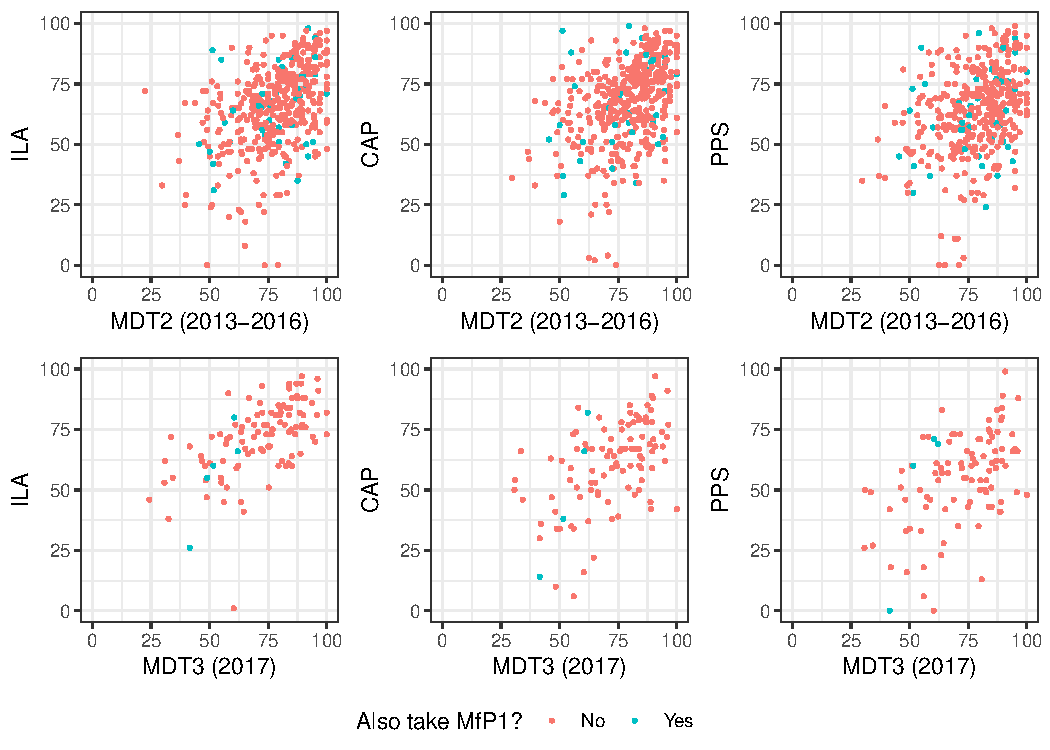
\includegraphics[width=\linewidth]{fig/REL_scatter_MfP1.pdf}
  \caption{\label{fig:REL_scatter_MfP1}Scatter plots of course results against MDT scores, grouped by the selection of MfP1}
\end{figure}

In Figure~\ref{fig:REL_splitbox} are shown the box plots of the course results grouped by MDT scores. Table~\ref{tab:REL_splitbox_anova} shows the summary table of ANOVA testing the null hypothesis that the mean of the course results for students scoring lower than 65 in MDT are equal. The non-significant probabilities do not reject the null hypotheses, i.e. there are no significant differences between the students taking MfP1 or not. 

\begin{figure}[H]
  \centering
  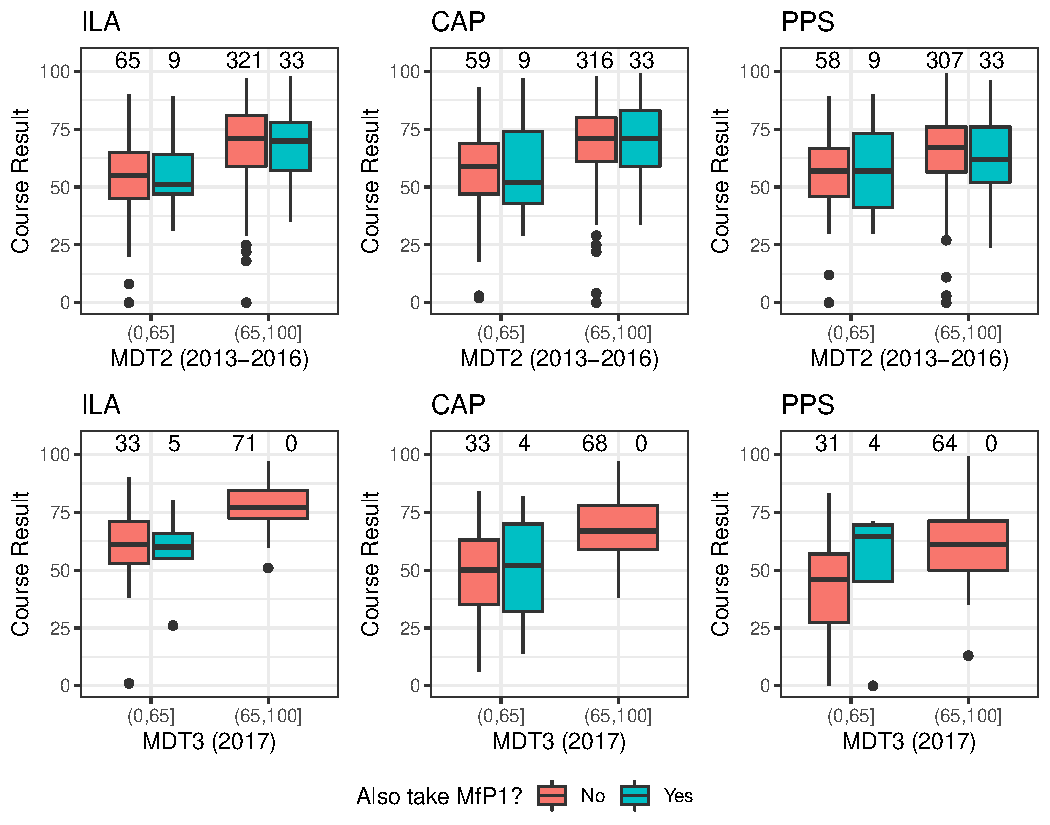
\includegraphics[width=\linewidth]{fig/REL_splitbox.pdf}
  \caption{\label{fig:REL_splitbox}Box plots of course results grouped by MDT scores}
\end{figure}

\begin{table}[ht]
  \centering
  \begin{tabular}{lrrrrr}
    \hline
   2013-2016 & Df & Sum Sq & Mean Sq & F value & Pr($>$F) \\ 
    \hline
  ILA.MfP1 & 1 & 209 & 208.87 & 0.661 & 0.419 \\ 
    Residuals & 72 & 22754 & 316.03 &  &  \\ 
     \hline
     \hline
     CAP.MfP1 & 1 & 33 & 33.33 & 0.088 & 0.768 \\ 
       Residuals & 66 & 25064 & 379.75 &  &  \\ 
    \hline
    \hline
    PPS.MfP1 & 1 & 35 & 34.79 & 0.098 & 0.755 \\ 
    Residuals & 65 & 23121 & 355.71 &  &  \\ 
      \hline
      \hline
     2017 & Df & Sum Sq & Mean Sq & F value & Pr($>$F) \\ 
       \hline
     ILA.MfP1 & 1 & 16 & 16.23 & 0.061 & 0.807 \\ 
       Residuals & 36 & 9613 & 267.01 &  &  \\ 
    \hline
    \hline
    CAP.MfP1 & 1 & 10 & 9.55 & 0.024 & 0.879 \\ 
    Residuals & 35 & 14226 & 406.45 &  &  \\ 
    \hline
    \hline
    PPS.MfP1 & 1 & 197 & 196.72 & 0.428 & 0.517 \\ 
      Residuals & 33 & 15166 & 459.57 &  &  \\ 
      \hline
  \end{tabular}
  \caption{\label{tab:REL_splitbox_anova}ANOVA table}
\end{table}

\section{Predictive modelling}

In Section~\ref{subsec:cm}, we make up the correlation between MDT scores and students' entry qualifications and use it as the feature of the binary classification that classify students in to `At-Risk' group and `Not-At-Risk' group. As suggested by Marbouti \cite{ml}, it is possible to identify students who are at-risk by using predictive modelling techniques from the field of machine learning. 

In this section, we introduce several machine learning techniques and use them to forecast the performance of students in Year 1 courses. Some \texttt{python} packages including \texttt{scikit-learn} and \texttt{NumPy} are used in the analyses. 

\subsection{Prediction methods}

Nine different prediction methods are used to identify at-risk students, which are described below. 

\begin{itemize}
\item Logistic Regression (LR), which was also used in the report last year, is used to predict the probability of getting over 50\% in the Year 1 courses. 
\item Naive Bayes (NB) Classifier, is a simple classifier based on Bayes' theorem with assumption of independent between the variables. This assumption is violated in this project, but this classifier still works when the dependencies of variables from each other are similar \cite{NBassump}. In this section, the distribution of each variable is assumed to be multinomial, because some the variables are categorical variables. 
\item K-Nearest Neighbour (KNN), is a non-parametric classifier, which classifies students based on their nearest neighbours. 
\item Multi-Layer Perceptron (MLP), is a kind of artificial neural network. In this section, two hidden layers with half of the number of observations as hidden nodes are used, as recommended by Marbouti \cite{ml}. 
\item Decision Tree (DT), is a non-parametric classifier classifying data with a set of if-then-else decision trees. In this section, a depth of 10 for the trees are chosen, because very fine splits are made involving very few data points when the trees are grown deeper and might overfit the data. 
\item Random Forest (RF), is constructed with multiple decision trees. 
\item Linear Support Vector Machine (SVM), finds a hyperplane separating the classes. 
\item Linear Discriminant Analysis (LDA), uses a maximum likelihood discrimination rule based on linear combinations and separates the classes with linear decision surface. 
\item Quadratic Discriminant Analysis (QDA), uses a maximum likelihood discrimination rule based on quadratic combinations and separates the classes with quadratic decision surface. 
\end{itemize}

To avoid accidentally over-fitting a model to the available data and generalising a poor fit to future data, we hold out a part of data as validation set and use the remaining part as training data. This is a statistical procedure called cross-validation. In particular, we use $K$-fold cross-validation for our data which is in short supply. The data is split into $K$ parts in the $K$-fold cross-validation procedure. Each model is fitted $K$ times with a different part of data used as a validation set and the remaining $K-1$ parts used for training. We then select the model with the lowest validation error, when averaged over $K$ folds. 

In this section, students' course results are fitted against the features (variables) that are available in the raw data set and significant (which is discussed in summer 2017 project) in the models we fit. These features include MDT mark, fee status group, school and gender. For the students from 2017, extra models which consider entry qualifications are also fitted. 

\subsection{Using MDT}

The normalised confusion matrices of different predictive models for each three Year 1 courses, given students admitted before 2017, are shown in Figure~\ref{fig:ML_ILA_bin_pre17}, Figure~\ref{fig:ML_CAP_bin_pre17} and Figure~\ref{fig:ML_PPS_bin_pre17}, while the entries of the original confusion matrices and the accuracies are shown in Table~\ref{tab:ML_ILA_bin_pre17}, Table~\ref{tab:ML_CAP_bin_pre17} and Table~\ref{tab:ML_PPS_bin_pre17}. Additionally, in Figure~\ref{fig:ML_Y1Fs_bin_pre17} is shown the normalised confusion matrices of models for risk status of students, with the corresponding confusion matrices and accuracies showing in Table~\ref{tab:ML_Y1Fs_bin_pre17}. 

The normalised confusion matrix is the marginal proportion of the original confusion matrix with regards to the true condition, which is summarised in Table~\ref{tab:cm_norm}. 

\begin{table}[ht]
  \centering
  \begin{tabular}{c|c|c|c}
    \hline
    \multicolumn{2}{c|}{} & \multicolumn{2}{c}{Predicted Condition} \\ 
    \cline{3-4}
    \multicolumn{2}{c|}{} & Positive & Negative \\ 
    \hline
  & & True Positive Rate & False Negative Rate \\ 
  & Positive & Sensitivity & Miss Rate \\ 
  True & & $\displaystyle TPR = \frac{TP}{TP+FN}$ & $\displaystyle FNR = \frac{FN}{TP+FN}$ \\
    \cline{2-4}
    Condition & & False Positive Rate & True Negative Rate \\ 
    & Negative & Fall-out & Specificity \\
    & & $\displaystyle FPR = \frac{FP}{TN+FP}$ & $\displaystyle TNR = \frac{TN}{TN+FP}$ \\
     \hline
  \end{tabular}
  \caption{\label{tab:cm_norm}Normalised confusion matrix}
\end{table}

It can be seen from the figures and tables that the accuracies of the models range from approximately 70\% to approximately 80\%. Among the nine models for each case, Naive Bayes Classifiers and K-Nearest Neighbour Classifiers have the highest true positive rates, which are approximately 50\%. However, these two models have the lowest true negative rates (around 20\%), indicating that more not-at-risk students are classified as at-risk students by these two models than the other. 

\newpage
\begin{figure}[H]
  \centering
  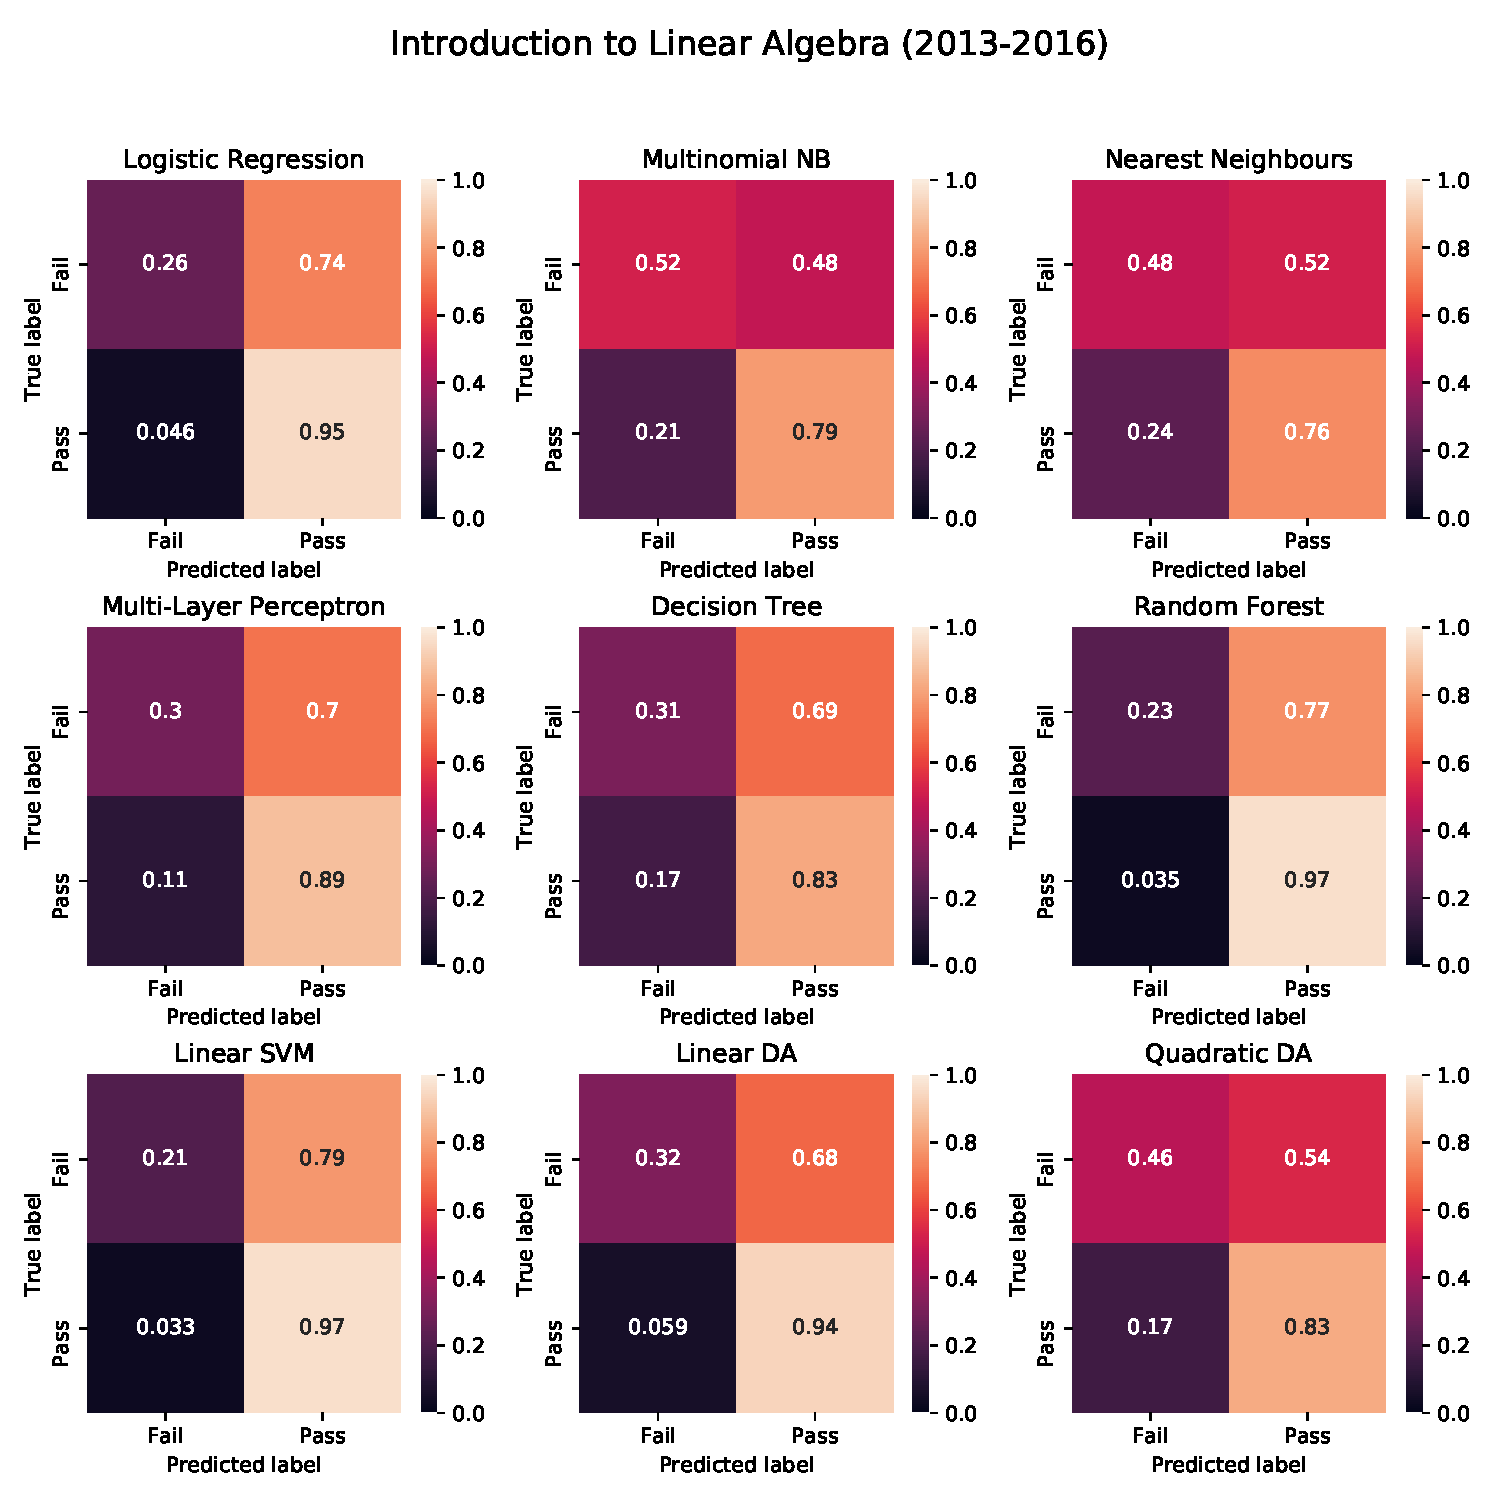
\includegraphics[width=\linewidth]{fig/ML_ILA_bin_pre17.pdf}
  \caption{\label{fig:ML_ILA_bin_pre17}Normalised confusion matrices of different prediction methods}
\end{figure}

\begin{table}[H]
  \centering
  \begin{tabular}{lrrrrrrrrr}
    \toprule
    {} &   LR &  MNB &  KNN &  MLP &   DT &   RF &  SVM &  LDA &  QDA \\
    \midrule
    TP  &   65 &  128 &  119 &   73 &   76 &   56 &   52 &   79 &  113 \\
    FN  &  181 &  118 &  127 &  173 &  170 &  190 &  194 &  167 &  133 \\
    FP  &   46 &  207 &  242 &  114 &  173 &   35 &   33 &   59 &  166 \\
    TN  &  958 &  797 &  762 &  890 &  831 &  969 &  971 &  945 &  838 \\
    ACC & 0.81 & 0.74 & 0.70 & 0.77 & 0.72 & 0.82 & 0.81 & 0.81 & 0.76 \\
    \bottomrule
  \end{tabular}
  \caption{\label{tab:ML_ILA_bin_pre17}Test results and accuracy of predictions}
\end{table}

\begin{figure}[H]
  \centering
  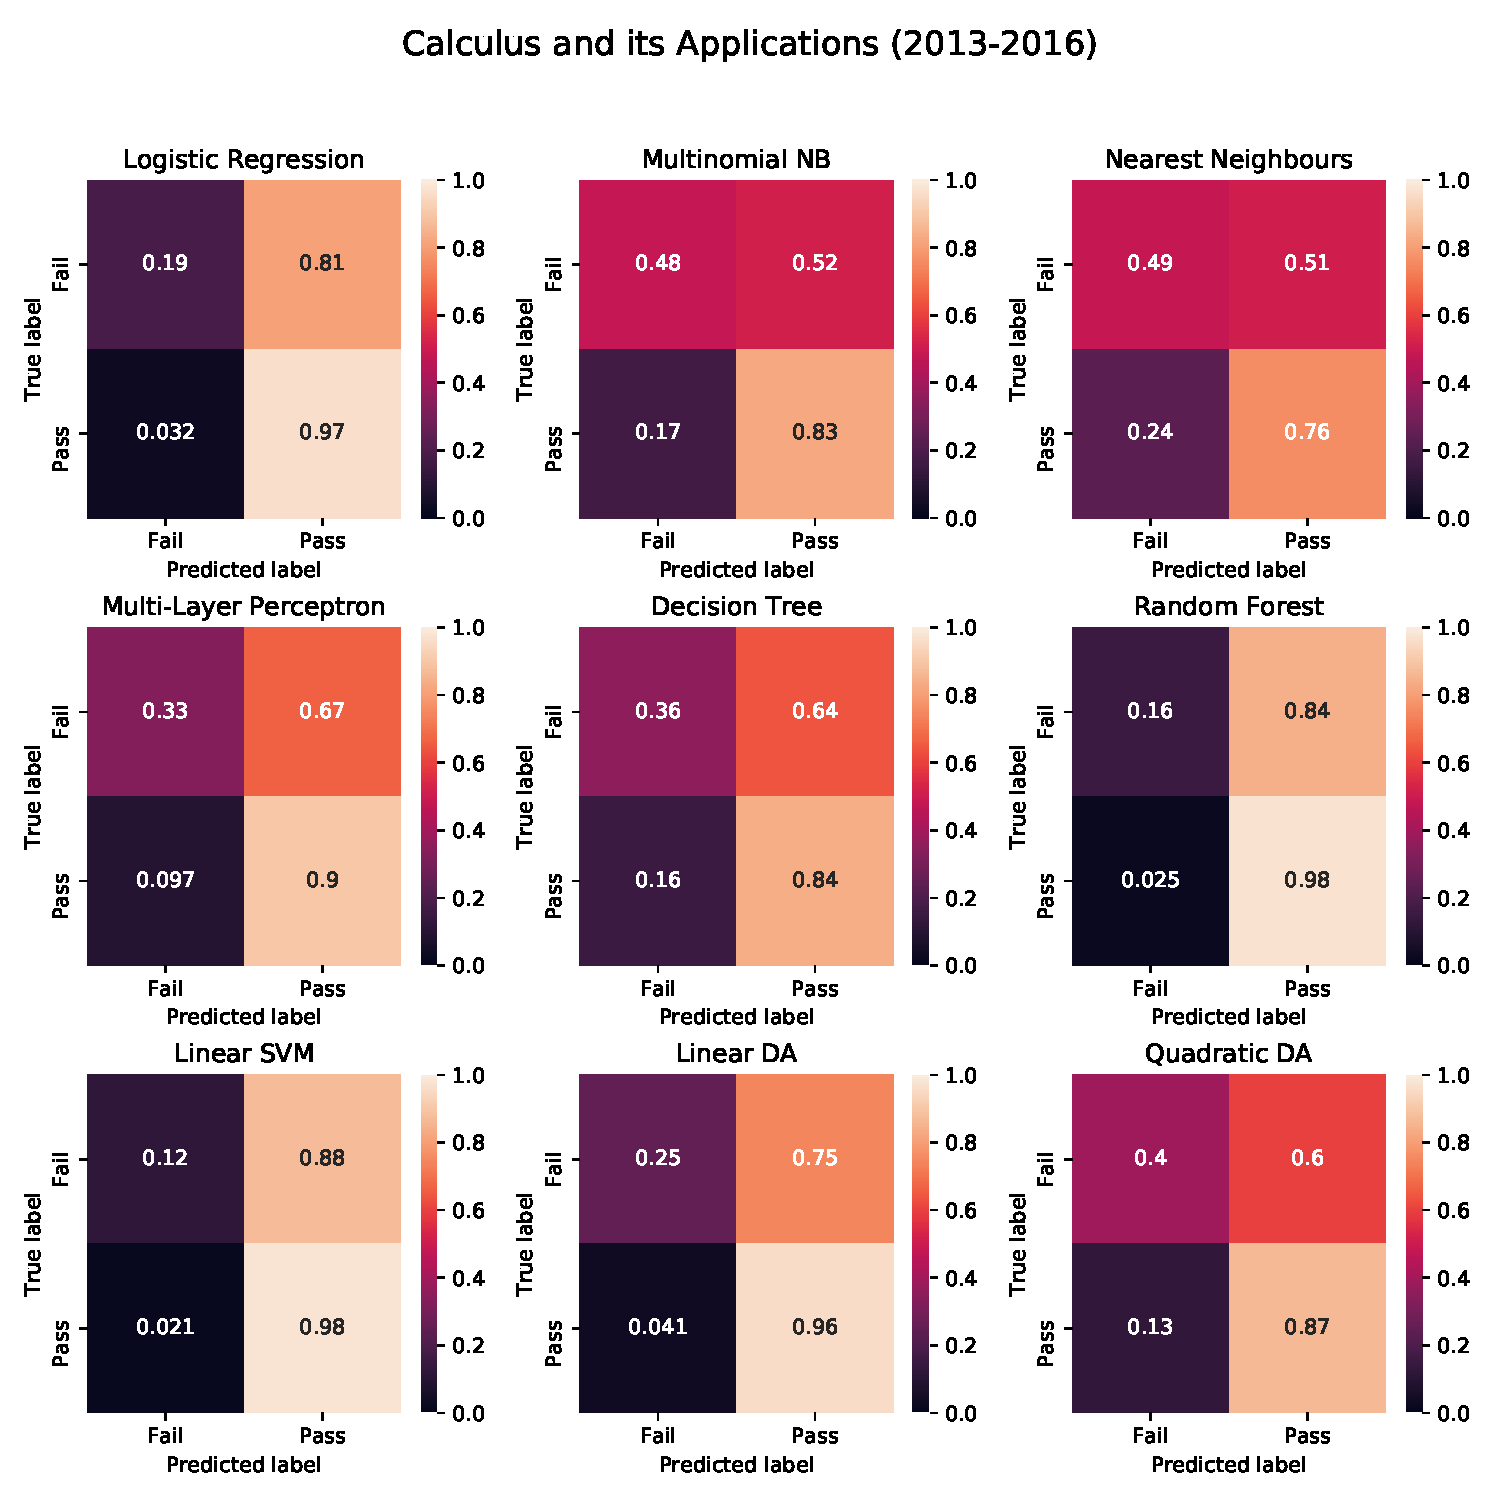
\includegraphics[width=\linewidth]{fig/ML_CAP_bin_pre17.pdf}
  \caption{\label{fig:ML_CAP_bin_pre17}Normalised confusion matrices of different prediction methods}
\end{figure}

\begin{table}[H]
  \centering
  \begin{tabular}{lrrrrrrrrr}
    \toprule
    {} &   LR &  MNB &  KNN &  MLP &   DT &   RF &  SVM &  LDA &  QDA \\
    \midrule
    TP  &   39 &   99 &  100 &   69 &   74 &   32 &   25 &   52 &   82 \\
    FN  &  167 &  107 &  106 &  137 &  132 &  174 &  181 &  154 &  124 \\
    FP  &   31 &  167 &  228 &   94 &  154 &   24 &   20 &   40 &  127 \\
    TN  &  936 &  800 &  739 &  873 &  813 &  943 &  947 &  927 &  840 \\
    ACC & 0.83 & 0.76 & 0.71 & 0.80 & 0.75 & 0.83 & 0.82 & 0.83 & 0.78 \\
    \bottomrule
  \end{tabular}
  \caption{\label{tab:ML_CAP_bin_pre17}Test results and accuracy of predictions}
\end{table}

\begin{figure}[H]
  \centering
  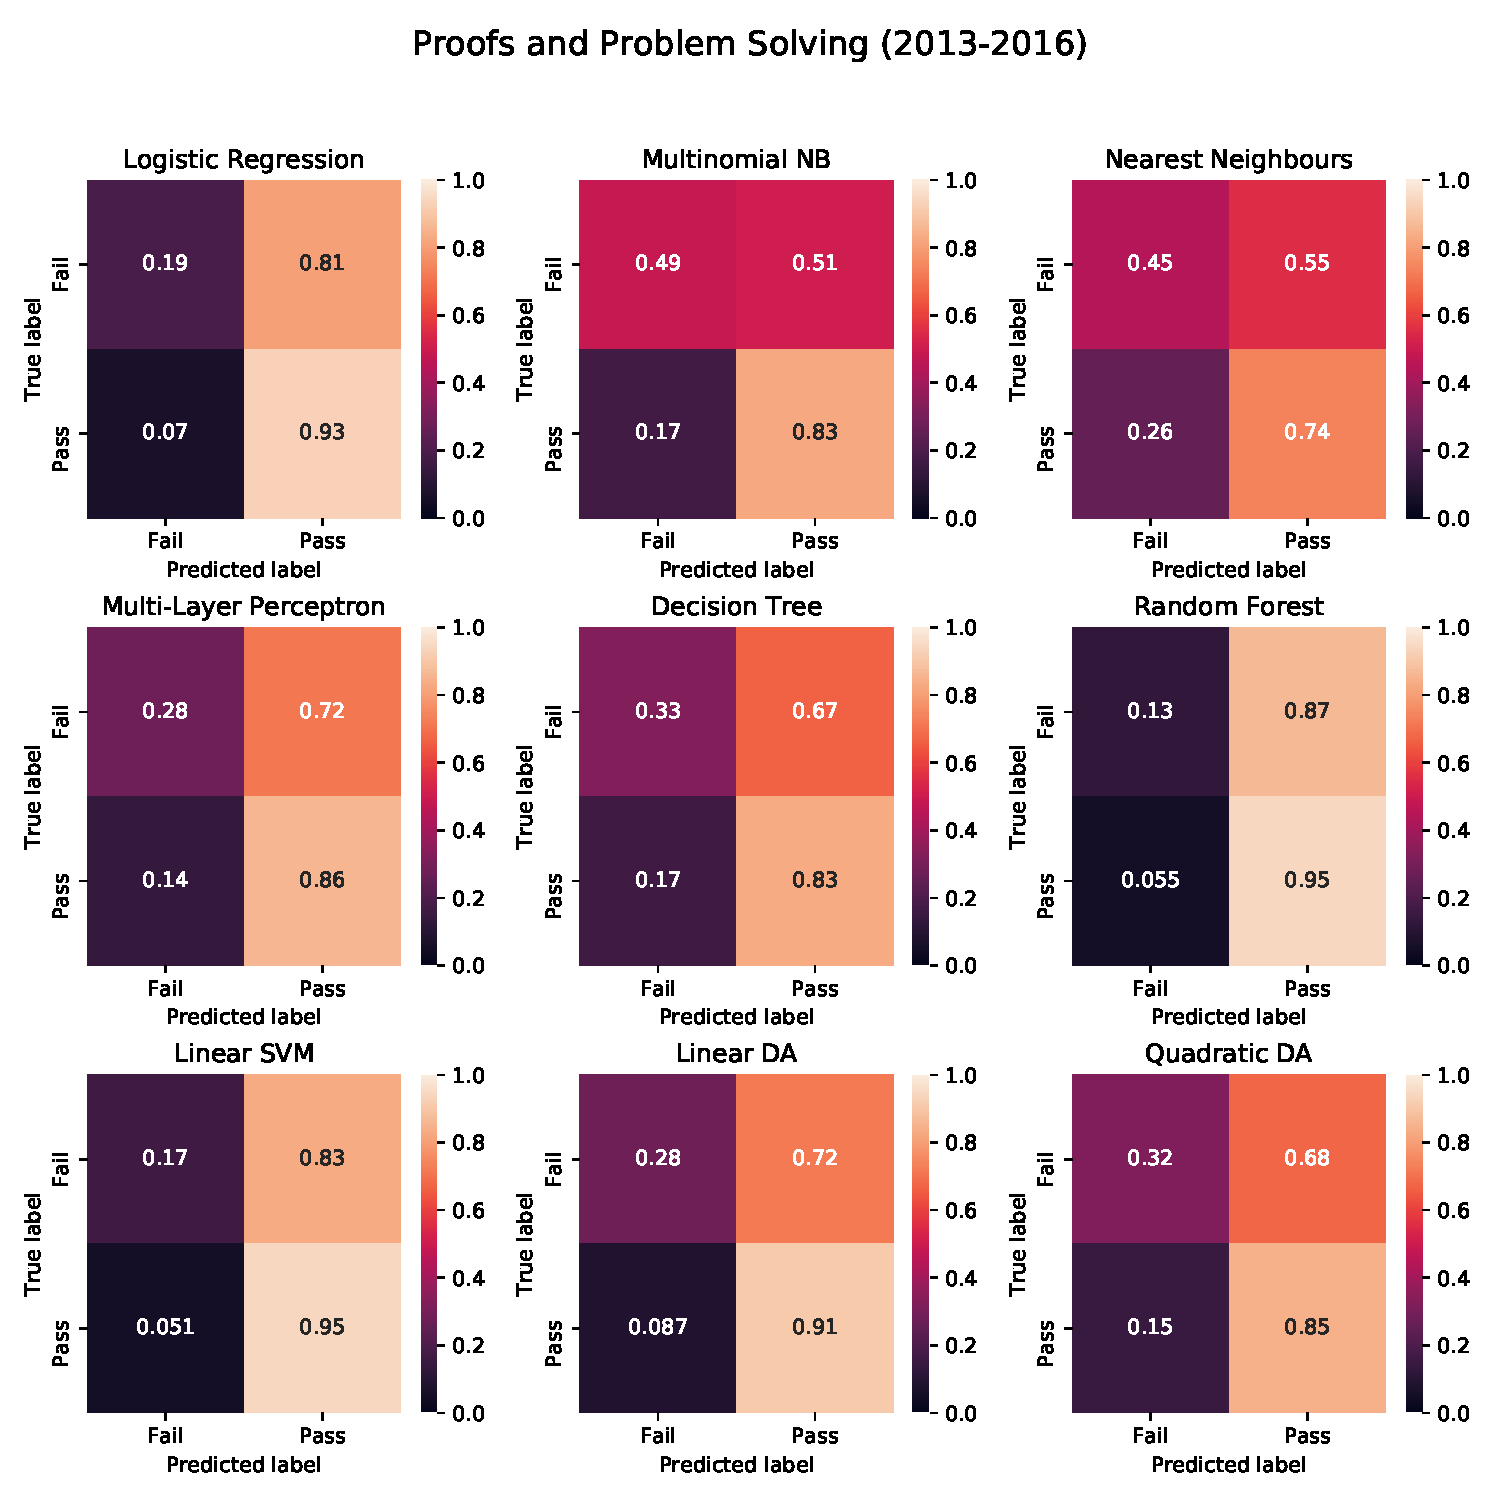
\includegraphics[width=\linewidth]{fig/ML_PPS_bin_pre17.pdf}
  \caption{\label{fig:ML_PPS_bin_pre17}Normalised confusion matrices of different prediction methods}
\end{figure}

\begin{table}[H]
  \centering
  \begin{tabular}{lrrrrrrrrr}
    \toprule
    {} &   LR &  MNB &  KNN &  MLP &   DT &   RF &  SVM &  LDA &  QDA \\
    \midrule
    TP  &   30 &   76 &   69 &   44 &   51 &   20 &   26 &   43 &   50 \\
    FN  &  125 &   79 &   86 &  111 &  104 &  135 &  129 &  112 &  105 \\
    FP  &   41 &  101 &  152 &   81 &   97 &   32 &   30 &   51 &   88 \\
    TN  &  546 &  486 &  435 &  506 &  490 &  555 &  557 &  536 &  499 \\
    ACC & 0.77 & 0.75 & 0.67 & 0.74 & 0.72 & 0.77 & 0.78 & 0.78 & 0.73 \\
    \bottomrule
  \end{tabular}
  \caption{\label{tab:ML_PPS_bin_pre17}Test results and accuracy of predictions}
\end{table}

\begin{figure}[H]
  \centering
  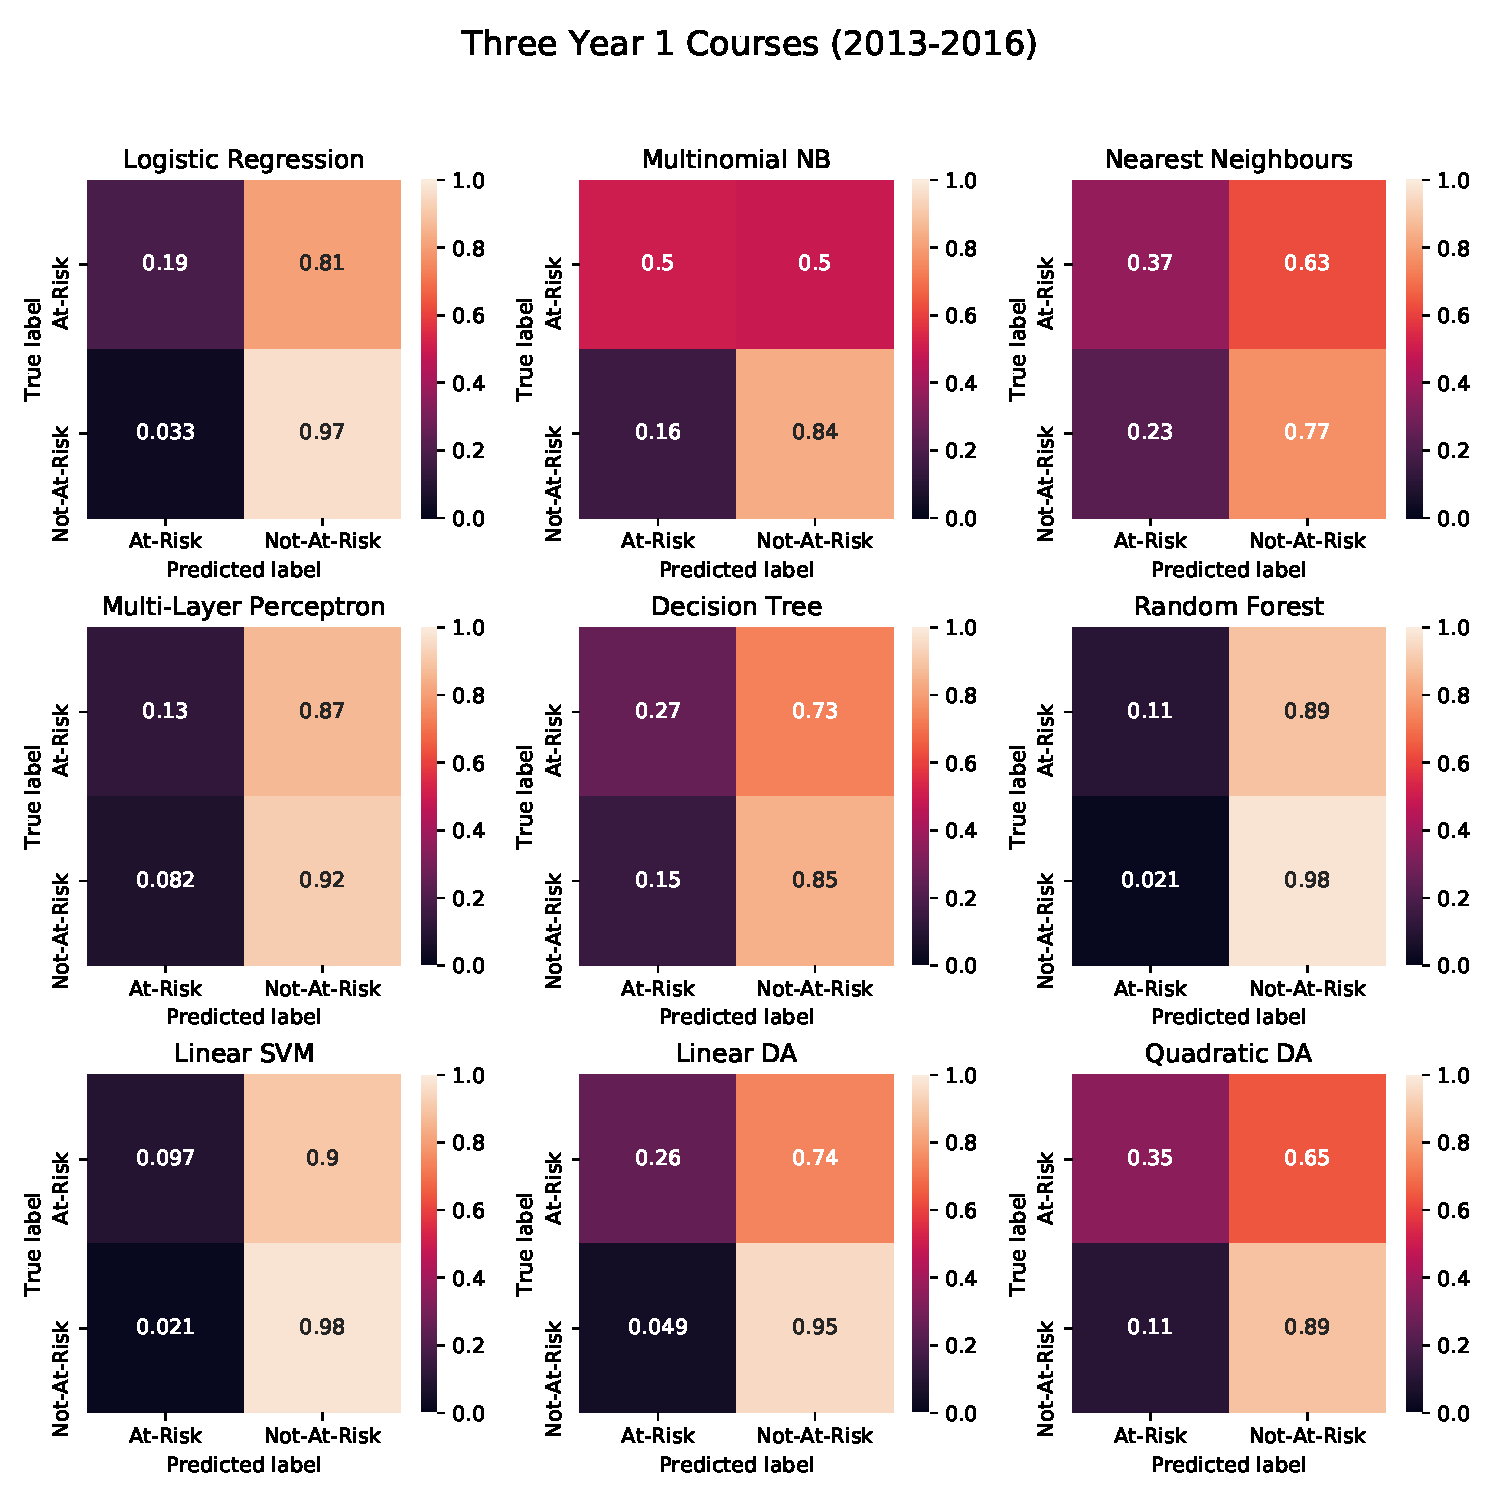
\includegraphics[width=\linewidth]{fig/ML_Y1Fs_bin_pre17.pdf}
  \caption{\label{fig:ML_Y1Fs_bin_pre17}Normalised confusion matrices of different prediction methods}
\end{figure}

\begin{table}[H]
  \centering
  \begin{tabular}{lrrrrrrrrr}
    \toprule
    {} &   LR &  MNB &  KNN &  MLP &   DT &   RF &  SVM &  LDA &  QDA \\
    \midrule
    TP  &   22 &   57 &   42 &   15 &   30 &   12 &   11 &   29 &   40 \\
    FN  &   91 &   56 &   71 &   98 &   83 &  101 &  102 &   84 &   73 \\
    FP  &   20 &  100 &  141 &   50 &   92 &   13 &   13 &   30 &   66 \\
    TN  &  591 &  511 &  470 &  561 &  519 &  598 &  598 &  581 &  545 \\
    ACC & 0.84 & 0.78 & 0.70 & 0.79 & 0.75 & 0.84 & 0.84 & 0.84 & 0.80 \\
    \bottomrule
  \end{tabular}
  \caption{\label{tab:ML_Y1Fs_bin_pre17}Test results and accuracy of predictions}
\end{table}

The normalised confusion matrices of different predictive models for each three Year 1 course, given students from 2017, are shown in Figure~\ref{fig:ML_ILA_bin_17}, Figure~\ref{fig:ML_CAP_bin_17} and Figure~\ref{fig:ML_PPS_bin_17}, while the entries of the original confusion matrices and the accuracies are shown in Table~\ref{tab:ML_ILA_bin_17}, Table~\ref{tab:ML_CAP_bin_17} and Table~\ref{tab:ML_PPS_bin_17}. Additionally, in Figure~\ref{fig:ML_Y1Fs_bin_17} is shown the normalised confusion matrices of models for risk status of students, with the corresponding confusion matrices and accuracies showing in Table~\ref{tab:ML_Y1Fs_bin_17}.  

The accuracies of models for ILA are higher compared to the models for students admitted before 2017. However, the contribution to the increased accuracies is mainly from the increase of true negative rates, while the true positive rates decrease. The accuracies and the true positive rates of the models for other courses are lower than the models for previous years. This may due to the short supply of data in 2017. 

\begin{figure}[H]
  \centering
  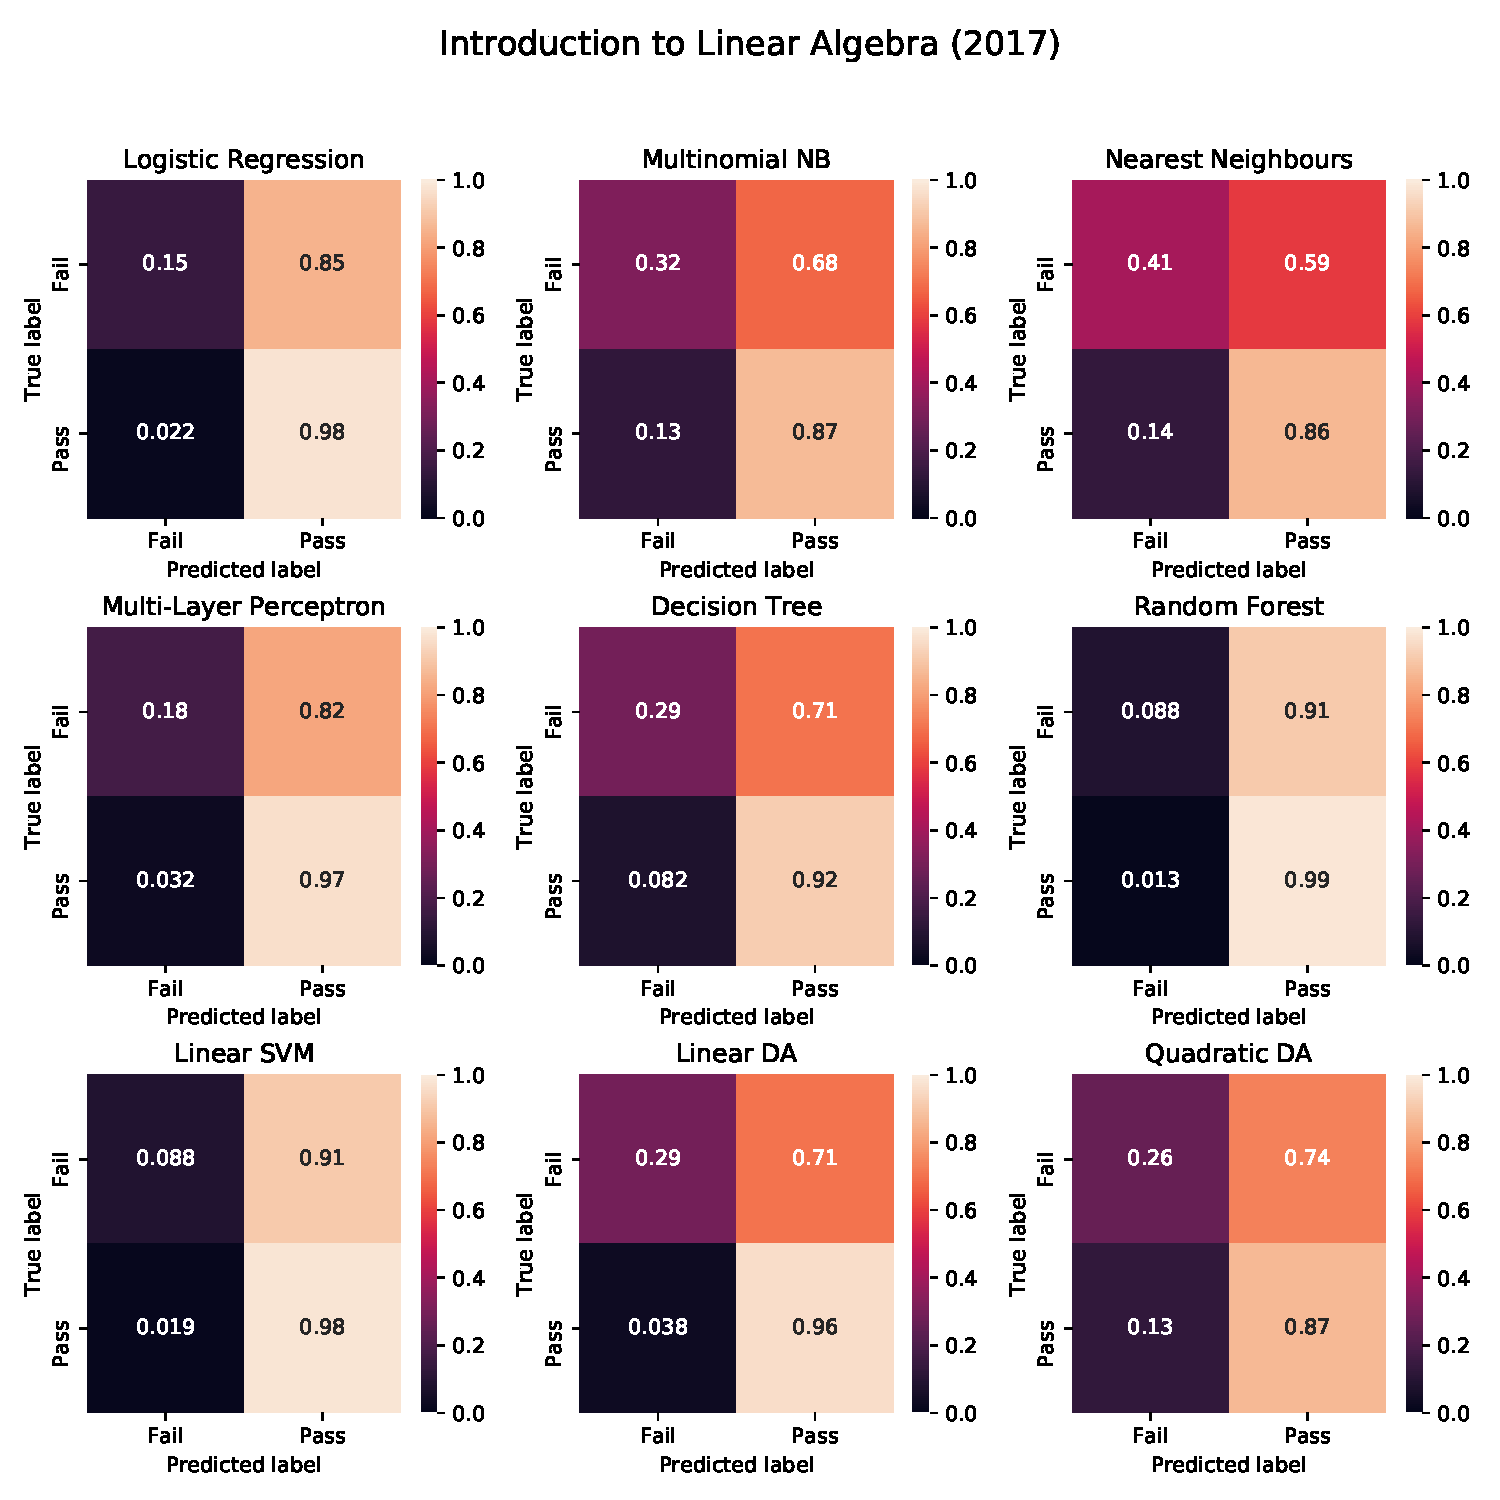
\includegraphics[width=\linewidth]{fig/ML_ILA_bin_17.pdf}
  \caption{\label{fig:ML_ILA_bin_17}Normalised confusion matrices of different prediction methods}
\end{figure}

\begin{table}[H]
  \centering
  \begin{tabular}{lrrrrrrrrr}
    \toprule
    {} &   LR &  MNB &  KNN &  MLP &   DT &   RF &  SVM &  LDA &  QDA \\
    \midrule
    TP  &    5 &   11 &   14 &    6 &   10 &    3 &    3 &   10 &    9 \\
    FN  &   29 &   23 &   20 &   28 &   24 &   31 &   31 &   24 &   25 \\
    FP  &    7 &   40 &   43 &   10 &   26 &    4 &    6 &   12 &   41 \\
    TN  &  310 &  277 &  274 &  307 &  291 &  313 &  311 &  305 &  276 \\
    ACC & 0.89 & 0.82 & 0.82 & 0.89 & 0.85 & 0.90 & 0.89 & 0.89 & 0.81 \\
    \bottomrule
  \end{tabular}
  \caption{\label{tab:ML_ILA_bin_17}Test results and accuracy of predictions}
\end{table}

\begin{figure}[H]
  \centering
  \includegraphics[width=\linewidth]{fig/ML_CAP_bin_17.pdf}
  \caption{\label{fig:ML_CAP_bin_17}Normalised confusion matrices of different prediction methods}
\end{figure}

\begin{table}[H]
  \centering
  \begin{tabular}{lrrrrrrrrr}
    \toprule
    {} &   LR &  MNB &  KNN &  MLP &   DT &   RF &  SVM &  LDA &  QDA \\
    \midrule
    TP  &   15 &   30 &   30 &   20 &   22 &   14 &   14 &   21 &   23 \\
    FN  &   49 &   34 &   34 &   44 &   42 &   50 &   50 &   43 &   41 \\
    FP  &   20 &   42 &   61 &   30 &   42 &   10 &   17 &   23 &   25 \\
    TN  &  237 &  215 &  196 &  227 &  215 &  247 &  240 &  234 &  232 \\
    ACC & 0.78 & 0.76 & 0.70 & 0.76 & 0.73 & 0.81 & 0.79 & 0.79 & 0.79 \\
    \bottomrule
  \end{tabular}
  \caption{\label{tab:ML_CAP_bin_17}Test results and accuracy of predictions}
\end{table}

\begin{figure}[H]
  \centering
  \includegraphics[width=\linewidth]{fig/ML_PPS_bin_17.pdf}
  \caption{\label{fig:ML_PPS_bin_17}Normalised confusion matrices of different prediction methods}
\end{figure}

\begin{table}[H]
  \centering
  \begin{tabular}{lrrrrrrrrr}
    \toprule
    {} &   LR &  MNB &  KNN &  MLP &   DT &   RF &  SVM &  LDA &  QDA \\
    \midrule
    TP  &   15 &   21 &   28 &   11 &   21 &   18 &   16 &   15 &   11 \\
    FN  &   39 &   33 &   26 &   43 &   33 &   36 &   38 &   39 &   43 \\
    FP  &   18 &   25 &   51 &   20 &   38 &   15 &   16 &   17 &   16 \\
    TN  &  124 &  117 &   91 &  122 &  104 &  127 &  126 &  125 &  126 \\
    ACC & 0.70 & 0.70 & 0.60 & 0.67 & 0.63 & 0.73 & 0.72 & 0.71 & 0.69 \\
    \bottomrule
  \end{tabular}
  \caption{\label{tab:ML_PPS_bin_17}Test results and accuracy of predictions}
\end{table}

\begin{figure}[H]
  \centering
  \includegraphics[width=\linewidth]{fig/ML_Y1Fs_bin_17.pdf}
  \caption{\label{fig:ML_Y1Fs_bin_17}Normalised confusion matrices of different prediction methods}
\end{figure}

\begin{table}[H]
  \centering
  \begin{tabular}{lrrrrrrrrr}
    \toprule
    {} &   LR &  MNB &  KNN &  MLP &   DT &   RF &  SVM &  LDA &  QDA \\
    \midrule
    TP  &    4 &    6 &    9 &    2 &    6 &    2 &    3 &    8 &    0 \\
    FN  &   20 &   18 &   15 &   22 &   18 &   22 &   21 &   16 &   24 \\
    FP  &   13 &   15 &   32 &   10 &   27 &    2 &   10 &   14 &    0 \\
    TN  &  146 &  144 &  127 &  149 &  132 &  157 &  149 &  145 &  159 \\
    ACC & 0.81 & 0.81 & 0.74 & 0.82 & 0.75 & 0.86 & 0.83 & 0.83 & 0.86 \\
    \bottomrule
  \end{tabular}
  \caption{\label{tab:ML_Y1Fs_bin_17}Test results and accuracy of predictions}
\end{table}

\subsection{Using both}

In Figure~\ref{fig:ML_ILA_bin_Qual_17}, Figure~\ref{fig:ML_CAP_bin_Qual_17}, Figure~\ref{fig:ML_PPS_bin_Qual_17} and Figure~\ref{fig:ML_Y1Fs_bin_Qual_17} are shown the normalised confusion matrices of the models which take students' entry qualifications into account. The corresponding confusion matrices and accuracies are shown in Table~\ref{tab:ML_ILA_bin_Qual_17}, Table~\ref{tab:ML_CAP_bin_Qual_17}, Table~\ref{tab:ML_PPS_bin_Qual_17} and Table~\ref{tab:ML_Y1Fs_bin_Qual_17}. 

The accuracies and true positive rates of these models are improved, compared with the models whose features do not include entry qualifications of students from 2017. However, the highest true positive rates of these models is only 50\%, which is not as high as expected. 

\begin{figure}[H]
  \centering
  \includegraphics[width=\linewidth]{fig/ML_ILA_bin_Qual_17.pdf}
  \caption{\label{fig:ML_ILA_bin_Qual_17}Normalised confusion matrices of different prediction methods}
\end{figure}

\begin{table}[H]
  \centering
  \begin{tabular}{lrrrrrrrrr}
    \toprule
    {} &   LR &  MNB &  KNN &  MLP &   DT &   RF &  SVM &  LDA &  QDA \\
    \midrule
    TP  &    6 &   12 &   14 &    3 &    8 &    3 &    3 &   10 &    8 \\
    FN  &   28 &   22 &   20 &   31 &   26 &   31 &   31 &   24 &   26 \\
    FP  &   11 &   38 &   44 &   12 &   33 &    3 &    8 &   15 &   34 \\
    TN  &  306 &  279 &  273 &  305 &  284 &  314 &  309 &  302 &  283 \\
    ACC & 0.88 & 0.82 & 0.81 & 0.87 & 0.83 & 0.90 & 0.88 & 0.88 & 0.82 \\
    \bottomrule
  \end{tabular}
  \caption{\label{tab:ML_ILA_bin_Qual_17}Test results and accuracy of predictions}
\end{table}

\begin{figure}[H]
  \centering
  \includegraphics[width=\linewidth]{fig/ML_CAP_bin_Qual_17.pdf}
  \caption{\label{fig:ML_CAP_bin_Qual_17}Normalised confusion matrices of different prediction methods}
\end{figure}

\begin{table}[H]
  \centering
  \begin{tabular}{lrrrrrrrrr}
    \toprule
    {} &   LR &  MNB &  KNN &  MLP &   DT &   RF &  SVM &  LDA &  QDA \\
    \midrule
    TP  &   19 &   30 &   32 &   19 &   21 &   18 &   17 &   23 &   23 \\
    FN  &   45 &   34 &   32 &   45 &   43 &   46 &   47 &   41 &   41 \\
    FP  &   23 &   34 &   59 &   27 &   46 &   10 &   19 &   23 &   21 \\
    TN  &  234 &  223 &  198 &  230 &  211 &  247 &  238 &  234 &  236 \\
    ACC & 0.78 & 0.78 & 0.71 & 0.77 & 0.72 & 0.82 & 0.79 & 0.80 & 0.80 \\
    \bottomrule
  \end{tabular}
  \caption{\label{tab:ML_CAP_bin_Qual_17}Test results and accuracy of predictions}
\end{table}

\begin{figure}[H]
  \centering
  \includegraphics[width=\linewidth]{fig/ML_PPS_bin_Qual_17.pdf}
  \caption{\label{fig:ML_PPS_bin_Qual_17}Normalised confusion matrices of different prediction methods}
\end{figure}

\begin{table}[H]
  \centering
  \begin{tabular}{lrrrrrrrrr}
    \toprule
    {} &   LR &  MNB &  KNN &  MLP &   DT &   RF &  SVM &  LDA &  QDA \\
    \midrule
    TP  &   18 &   22 &   27 &   22 &   20 &   11 &   16 &   16 &   24 \\
    FN  &   36 &   32 &   27 &   32 &   34 &   43 &   38 &   38 &   30 \\
    FP  &   19 &   24 &   49 &   28 &   34 &   10 &   15 &   19 &   26 \\
    TN  &  123 &  118 &   93 &  114 &  108 &  132 &  127 &  123 &  116 \\
    ACC & 0.71 & 0.71 & 0.61 & 0.69 & 0.65 & 0.72 & 0.72 & 0.70 & 0.71 \\
    \bottomrule
  \end{tabular}
  \caption{\label{tab:ML_PPS_bin_Qual_17}Test results and accuracy of predictions}
\end{table}

\begin{figure}[H]
  \centering
  \includegraphics[width=\linewidth]{fig/ML_Y1Fs_bin_Qual_17.pdf}
  \caption{\label{fig:ML_Y1Fs_bin_Qual_17}Normalised confusion matrices of different prediction methods}
\end{figure}

\begin{table}[H]
  \centering
  \begin{tabular}{lrrrrrrrrr}
    \toprule
    {} &   LR &  MNB &  KNN &  MLP &   DT &   RF &  SVM &  LDA &  QDA \\
    \midrule
    TP  &    8 &    8 &    9 &    5 &    9 &    4 &    6 &    6 &    0 \\
    FN  &   16 &   16 &   15 &   19 &   15 &   20 &   18 &   18 &   24 \\
    FP  &   14 &   17 &   32 &    5 &   23 &    3 &    9 &   12 &    0 \\
    TN  &  145 &  142 &  127 &  154 &  136 &  156 &  150 &  147 &  159 \\
    ACC & 0.83 & 0.81 & 0.74 & 0.86 & 0.79 & 0.87 & 0.85 & 0.83 & 0.86 \\
    \bottomrule
  \end{tabular}
  \caption{\label{tab:ML_Y1Fs_bin_Qual_17}Test results and accuracy of predictions}
\end{table}

\subsection{Summary}

Compared to the binary classification using stacked bar plots described in Section~\ref{sec:stackbar_binclf}, using the predictive models earlier this section does not improve the performance of classification of the students. This may due to several problems involved in the predictive models. 

\begin{itemize}
\item The population of the data set, especially the data for students from 2017, is quite small and does not enough for training the predictive models. When fitting Quadratic Discriminant Analysis model for students from 2017, we are warned by the \texttt{python} package that the variables are collinear. 
\item The categorical variables are converted to ordinal variables. For example, using natural ordering in variables fee status group and school may result in bad performance, because no ordinal relationship exists in these variables. Alternatively, they should be represented using binary vectors, i.e. using `one-hot' (also known as `one-of-$k$') encoding. 
\end{itemize}

Additionally, the predictive models used in this section are based on the recommendation from Marbouti \cite{ml} and we do not have further exploration of how to improve the models because of time limitation in this summer project. However, as the number of students taking MDT increases, and the performance of the predictive models improves, using machine learning methods would have better prediction and classification of students based on their risk status than using visual representation from the stacked bar plots. 


\nocite{*} % includes ref aren't cited
%\bibliographystyle{acm} % check style
\newpage
\addcontentsline{toc}{chapter}{Bibliography}
\printbibliography

\end{document}